\documentclass[11pt]{article}
\usepackage[margin=2.54cm]{geometry}
\usepackage[dvipsnames,usenames]{color}
\usepackage{amsfonts,amsmath,amssymb,amsthm,mathtools}
\usepackage{paralist}
\usepackage{algorithmic,algorithm}
\usepackage{bm}
\usepackage{xspace}
\usepackage{centernot}
\usepackage{fancybox}
\usepackage{framed}

%\usepackage{mathabx}
\usepackage[pagebackref,letterpaper=true,colorlinks=true,pdfpagemode=none,urlcolor=blue,linkcolor=blue,citecolor=BrickRed,pdfstartview=FitH]{hyperref}
\usepackage{xspace,prettyref}
\usepackage{color}
\usepackage{graphics}
%\usepackage{MnSymbol}
%% For hyperlinks. Should always be the last package.
%\usepackage[colorlinks,urlcolor=blue,citecolor=blue,linkcolor=blue]{hyperref}
\let\pref=\prettyref
\newcommand{\mathcalavehyperref}[2]{\texorpdfstring{\hyperref[#1]{#2}}{#2}}
\newcommand{\comment}[1]{ {\color{BrickRed} \footnotesize[#1]}\marginpar{\footnotesize\textbf{\color{red} To Do!}}}
\newcommand{\ignore}[1]{}


\newtheorem{theorem}{Theorem}
\newtheorem{lemmata}[theorem]{Lemmata}
\newtheorem{lemma}[theorem]{Lemma}
\newtheorem{claim}[theorem]{Claim}
\newtheorem{subclaim}{Subclaim}
\newtheorem{proposition}[theorem]{Proposition}
\newtheorem{corollary}[theorem]{Corollary}
\newtheorem{fact}[theorem]{Fact}
\newtheorem{conjecture}[theorem]{Conjecture}
\newtheorem{question}[theorem]{Question}
\newtheorem{example}[theorem]{Example}
\newtheorem{definition}[theorem]{Definition}
\theoremstyle{definition}
\newtheorem{remark}{Remark}
\newtheorem{observation}{Observation}


\newcommand{\EPSfigure}[5]{

        % #1 = File name and other arguments to \psfig macro
        % #2 = Caption Text
        % #3 = Positioning Letters: h, t|b|p
        % #4 = {*} causes double column figure, {} for single
        % #5 = Label to apply to figure

        \begin{figure#4}[#3]
                \centering
                \ \psfig{file=#1}
%               \label{#5}
%
                \ \caption{{\em #2}\label{#5}}\hfill\break

        \end{figure#4}
}

\newcommand{\innbd}{\Gamma^-}
\newcommand{\nbd}{\Gamma}
\newcommand{\outnbd}{\Gamma^+}

\newcommand{\bT}{{\bf T}}

\newcommand{\cA}{{\cal A}}
\newcommand{\cB}{{\cal B}}
\newcommand{\cC}{{\cal C}}
\newcommand{\cD}{{\cal D}}
\newcommand{\cE}{{\cal E}}
\newcommand{\cF}{{\cal F}}
\newcommand{\cG}{{\cal G}}
\newcommand{\cH}{{\cal H}}
\newcommand{\cJ}{{\cal J}}
\newcommand{\cL}{{\cal L}}
\newcommand{\cP}{{\cal P}}
\newcommand{\cS}{{\cal S}}
\newcommand{\cU}{{\cal U}}
\newcommand{\cV}{{\cal V}}

\newcommand{\LL}{\mathbb{L}}
\newcommand{\MM}{\mathbb{M}}
\newcommand{\NN}{\mathbb{N}}
\newcommand{\PP}{\mathbb{P}}
\newcommand{\RR}{\mathbb{R}}
\newcommand{\SSS}{\mathbb{S}}



\newcommand{\bmu}{\overline{\mu}}
\newcommand{\poly}{\textrm{poly}}
\newcommand{\mymod}{\textrm{mod} \ }
\newcommand{\otilde}{\widetilde{O}}
%\newcommand{\qed}{\hfill $\Box$}
\newcommand{\eps}{\varepsilon}
\newcommand{\fu}{\varphi}
\newcommand{\restr}[1]{{|_{{\textstyle #1}}}}
\newcommand{\proj}{\mbox{\rm proj}}
\newcommand{\vol}{\mbox{\tt vol}\,}
\newcommand{\area}{\mbox{\tt area}\,}
\newcommand{\conv}{\mbox{\tt conv}\,}
\newcommand{\diam}{\hbox{\tt diam}\,}
\newcommand{\hdisc}{\mbox{\rm herdisc}}
\newcommand{\ldisc}{\mbox{\rm lindisc}}
\newcommand{\EX}{\hbox{\bf E}}
\newcommand{\prob}{{\rm Prob}}
\newcommand{\proofend}{{\medskip\medskip}}
%\newcommand{\proof}{{\noindent\bf Proof: }}
%\newcommand{\reals}{{\rm I\!\hspace{-0.025em} R}}
%\newcommand{\dist}{\hbox{dist}}
\newcommand{\defeq}{\mbox{\,$\stackrel{\rm def}{=}$\,}}
\newcommand{\boxalg}[1]
{\begin{center}\fbox{\parbox{\columnwidth}{\tt
\begin{tabbing}
\=mm\=mm\=mm\=mm\=mm\=mm\=mm\=mm\=mm\kill
#1
\end{tabbing} } } \end{center} }

%% HYPER-LINKED REFERENCES
\newcommand{\Sec}[1]{\hyperref[sec:#1]{\S\ref*{sec:#1}}} %section
\newcommand{\Eqn}[1]{\hyperref[eqn:#1]{(\ref*{eqn:#1})}} %equation
\newcommand{\Clm}[1]{\hyperref[clm:#1]{Claim~\ref*{clm:#1}}} %claim
\newcommand{\Fig}[1]{\hyperref[fig:#1]{Figure~\ref*{fig:#1}}} %figure
\newcommand{\Tab}[1]{\hyperref[tab:#1]{Table~\ref*{tab:#1}}} %table
\newcommand{\Thm}[1]{\hyperref[thm:#1]{Theorem~\ref*{thm:#1}}} %theorem
\newcommand{\Lem}[1]{\hyperref[lem:#1]{Lemma~\ref*{lem:#1}}} %lemma
\newcommand{\Prop}[1]{\hyperref[prop:#1]{Proposition~\ref*{prop:#1}}} %property
\newcommand{\Cor}[1]{\hyperref[cor:#1]{Corollary~\ref*{cor:#1}}} %corollary
\newcommand{\Def}[1]{\hyperref[def:#1]{Definition~\ref*{def:#1}}} %definition
\newcommand{\Alg}[1]{\hyperref[alg:#1]{Algorithm~\ref*{alg:#1}}} %algorithm
\newcommand{\Ex}[1]{\hyperref[ex:#1]{Example~\ref*{ex:#1}}} %example
\newcommand{\Obs}[1]{\hyperref[obs:#1]{Observation~\ref*{obs:#1}}} %observation

%% Comments to ourselves
\newcommand{\Reminder}[1]{{\color{red}#1}}
\newcommand{\Sesh}[1]{\Reminder{Sesh interjects: #1}}

%%Ben Added
\DefineNamedColor{named}{RedViolet} {cmyk}{0.07,0.90,0,0.34}
\providecommand{\AlgorithmI}[1]{{\textcolor[named]{RedViolet}{\texttt{\bf{#1}}}}}
\providecommand{\Algorithm}[1]{{\AlgorithmI{#1}\index{algorithm!#1@{\AlgorithmI{#1}}}}}
\newcommand{\zip}{\Algorithm{ZIP}}
\newcommand{\link}{\Algorithm{LINK}}
\newcommand{\sizes}{\Algorithm{SIZES}}
\newcommand{\AMT}{\ensuremath{\mathsf{AMT}}\xspace}
\newcommand{\MT}{\ensuremath{\mathsf{MT}}\xspace}
\newcommand{\BCS}{\ensuremath{\mathsf{BCS}}\xspace}
\newcommand{\sub}{\mathsf{sub}}
\newcommand{\Merge}{\mathsf{Merge}}
\newcommand{\stack}{\mathsf{S}}
\newcommand{\AQ}{\mathsf{AQ}}

\newcommand{\etal}{\textit{et~al.}\xspace}

\newcommand{\build}{{\tt build}}
\newcommand{\col}{col}
\newcommand{\fcol}{full}
\newcommand{\cur}{cur}
\newcommand{\cut}{{\tt cut}}
\newcommand{\cont}{\psi}
\newcommand{\cost}{\mathop{cost}}
\newcommand{\h}{att}
\newcommand{\init}{{\tt init}}
\newcommand{\jc}{\cJ_C}
\newcommand{\lift}{{\tt lift}}
\newcommand{\mcol}{mcol}
\newcommand{\merge}{{\tt merge}}
\newcommand{\onestep}{{\tt piece}}
\newcommand{\paint}{{\tt paint}}
\newcommand{\pal}{P}
\newcommand{\pmax}{P_{\max}}
\newcommand{\rain}{{\tt rain}}
\newcommand{\reeb}{\cC}
\newcommand{\redH}{\widetilde{H}}
\newcommand{\rep}{rep}
\newcommand{\st}{K}
\newcommand{\surgery}{{\tt surgery}}
\newcommand{\touch}{T}
\newcommand{\update}{{\tt update}}
\newcommand{\wet}{{\tt wet}}

\newcommand{\MTAlg}{\Algorithm{MTAlg}\xspace}
\newcommand{\Init}{\Algorithm{Init}\xspace}

\newcommand{\CodeComment}[1]{\textcolor{blue}{\texttt{#1}}}


\newcommand{\XSays}[2]{{
      {$\rule[-0.12cm]{0.2in}{0.5cm}$\fbox{\tt
            #1:} }
      \textcolor{red}{#2}
      \marginpar{\textcolor{blue}{#1}}
      {$\rule[0.1cm]{0.3in}{0.1cm}$\fbox{\tt
            end}$\rule[0.1cm]{0.3in}{0.1cm}$}
      }
   }
\newcommand{\Ben}[1]{{\XSays{Ben}{#1}}}
\newcommand{\remove}[1]{}
\newcommand{\pth}[2][\!]{#1\left({#2}\right)}



\author{
  Benjamin Raichel
  \and
  C. Seshadhri
}

\title{A Mountaintop View Requires Minimal Sorting: \break An Instance Optimal Contour Tree Algorithm}
\date{}


\begin{document}

\maketitle

\begin{abstract}
Reeb graphs are a fundamental topological structure which tracks the evolution of levels sets of a real valued function over a manifold.  
In the case when this graph is loop free it is called a contour tree.  Due to the use of the contour trees in practice on large data sets, 
there has been significant previous work in developing algorithms for their efficient computation. 

Here we present the first contour tree algorithm which takes into account the shape of the contour tree, 
and in doing so yields instance optimal results.
Specifically, we prove that for any partition of the contour tree into a set of descending paths, $P$, 
any comparison based algorithm requires $\sum_{p\in P} |p|\log|p|$ time.  Moreover, we show there   
exists some partition $P'$ such that the running time of our algorithm is 
$O(\sum_{p\in P'} |p|\log|p| + N\alpha(N))$, where $N$ is the total complexity of the input manifold 
(and hence this is optimal on all instances requiring $\Omega(N\alpha(N))$ time).
In particular, our algorithm runs in $O(N\alpha(N))$ time when the tree is balanced, 
while previous algorithms ran in $O(N+t\log t)$ (where $t$ is the size of the contour tree).
%In particular, our algorithm runs in $O(N\alpha(N))$ time when the tree is balanced, yet still 
%matches the previous worst case $O(N+n\log n)$ bound when the tree is long and skinny.

In order to produce our instance optimal results we introduce a novel linear time surface partitioning scheme which is likely to have applications elsewhere.
Moreover, in order to prove the optimality we use a non-trivial combinatorial discharging argument which we believe is of independent interest and in particular uses 
such tools as heavy-light path decompositions.
\end{abstract}


\section{Introduction}

Let $f$ be a real valued function defined over a manifold embedded in $\RR^d$.  
For any real value $\alpha$, the level set $f^{-1}(\alpha)$ can be decomposed into its connected components, or ``contours''.
The Reeb graph is a fundamental topological structure which represents the evolution of these contours as one sweeps the surface 
from $-\infty$ to $\infty$ according to $f$.  Often this graph is acyclic, in which case it is 
called a \emph{contour tree}.  This is the case if, for example, the input is a surface mesh of a mountain range 
(and the contour tree would encode when mountain peeks form and how they merge together).

There is a long list of practical applications of the study of contour trees (see for example \cite{c-tmi-04} and references therein).
Often these applications involve massive data sets, and so consequently there has also been a long series 
of results on efficient algorithms for their computation \cite{kobps-ctsssit-97,tv-cct-98,csa-cctad-00,pc-ectls-02,cllr-sooscctmp-05}.
Let $N$ be the total size of the input manifold, $n$ the number of vertices, and $t$ the number of critical points. (Note that in many applications $N=O(n)$.)
As an initial step these algorithms require that all $t$ contour tree vertices be sorted.  
In particular, \cite{cllr-sooscctmp-05} provide an $O(N+t\log t)$ time algorithm, and since in the worst case computing the contour tree 
requires $\Omega(N+t\log t)$ time, this algorithm is optimal with respect to the size of the output.  
Here we present the first contour tree algorithm which is optimal (for instances requiring $\Omega(N\alpha(N))$ 
time\footnote{Where $\alpha(\cdot)$ is the inverse Ackermann function, which is $< 5$ for computation in this universe.}) 
with respect not just to the size of the output, but also its structure.  This is accomplished by introducing a simple linear time 
surface partitioning scheme to avoid sorting, which is likely to have applications elsewhere.  
For all instances the bound for our algorithm either matches the best previous bound, or is faster.
For, example when the contour tree is a balanced, our algorithm runs in $O(N\alpha(N))$ time, whereas all 
previous algorithms had a running time of $\Omega(N+t\log t)$

%In particular, the algorithm in \cite{cllr-sooscctmp-05} is worst case optimal with respect to the size of the output.  
%Here we present the first contour tree algorithm which is (near\footnote{Our algorithm is optimal on all instance requiring $\Omega(n\alpha(n))$ time.}) 
%optimal with respect not just to the size of the output, but also its structure.  
%Specifically, the bound for our algorithm either matches \cite{cllr-sooscctmp-05}, or is faster.
%For, example when the contour tree is a balanced, our algorithm runs in $O(n\alpha(n))$ time, whereas all 
%previous algorithms had a running time of $\Omega(n\log n)$.

This work can be seen as a continuation of the study of instance-optimal geometric algorithms introduced by Afshani \etal \cite{abc-ioga-09}.
In order to prove instance optimality we use a non-trivial combinatorial discharging argument, which we believe is of independent interest.
Of particular note is the use of heavy-light path decompositions, first introduced by Sleator and Tarjan \cite{st-dsdt-83} in their analysis of link-cut trees.



% Explain why useful:  Lets you know the ``shape of your date''.  Map of the critical points where contours change.  
%Fast extraction of seed sets in a small sized structure, which can let you do threshold queries.
% 
% \medskip\noindent
% Paragraph on specific applications.  Scientific visualization, in particular combustion research.  GIS.

\subsection{Previous Work}

\subsubsection{Worst Case Alternatives}
In worst case analysis an algorithm's running time is judged in terms of its worst 
case behavior over all inputs of a given size.  While there are benefits to this viewpoint, 
such as robustness,  it fails to capture the whole story.  As such, many alternatives 
have been considered.  For example, one can make assumptions on the distribution of 
inputs, which has led to a number interesting results on average case and probabilistic 
analysis, and also smoothed analysis \cite{st-saa-04}.  However, even without making 
assumptions on the distribution of the input, there is still more to the story.
For example, in the study of parametrized complexity, one takes into account other 
parameters determined by the input other than just its size (for example the maximum 
degree in a graph or whether it is planar).

\paragraph{Output Sensitive Analysis.}
In geometric settings often the goal is to compute a (potentially complex) geometric structure determined 
by the input, and so it is natural to also consider how the form of this output structure affects the running time.
One example is the standard sweep line algorithm of Bentley and Ottmann \cite{bo-arcgi-79} for line segment intersection, 
which runs $O((n+k)\log n)$ time where k is the number of intersections, which in the worst case is quadratic.
Another example is Chan's algorithm for computing the convex hull \cite{c-ooscha-96} which runs in $O(n\log h)$ 
where $h$ is the number of vertices on the hull, which in the worst case is $n$.  While such algorithms represent 
significant improvements over their worst case counterparts, their running times are only measured with respect 
to the size of the output and not any structure it may have.

\paragraph{Instance Optimality.}  
Here we are concerned with a more refined analysis than the typical output sensitive analysis.
Specifically, we investigate an algorithm which is instance optimal as defined by Afshani \etal \cite{abc-ioga-09}.  
In order to prove such a result, one considers a family of allowable partitions of the input, 
each of which is defined in terms of the structure of the output.  Each such partition then has 
an associated entropy type cost representing the number of possible instantiations of such a partition.
Our work differs slightly from Afshani \etal \cite{abc-ioga-09} however, in that they show any algorithm 
(for say the convex hull) requires the minimum such cost, where as in our case it is shown that 
any algorithm requires the maximum over these costs.


\subsubsection{Contour Trees}

\Ben{Maybe discuss contour tree applications and why they are useful here? Or maybe earlier?}

\paragraph{A History of Contour Trees.}
As discussed above, there has been a long series of improved algorithms for computing contour trees.
Kreveld \etal \cite{kobps-ctsssit-97} presented an $O(N\log N)$ time algorithm for functions over 2D 
meshes and an $O(N^2)$ algorithm for higher dimensions, where $N$ is the number of simplices in the mesh. 
Tarasov and Vyalya \cite{tv-cct-98} improved the running time to $O(N\log N)$ for the 3D case by making 
several passes over the input.

Carr \etal \cite{csa-cctad-00} improved the running time for all dimensions to $O(n\log n + N)$, 
where $n$ is the number of mesh vertices.  Their algorithm works in 3 simple stages.  
The first stage consist of a top down sweep to compute what is known as the join (or merge) tree, 
which tracks the evolution of super-level sets (whereas the contour tree tracks level sets).  
Similarly, the second stage does a bottom up sweep to compute the split tree, which tracks sub-level sets.  
Their main contribution is the third and final step where they present an $O(n)$ time algorithm to merge 
together the join and split trees to get the contour tree.  

There have also been some output sensitive results for computing the contour tree.  Let $t$ be the number 
of critical points in the input mesh, which could potentially be much smaller than $n$.  
Cole-McLaughlin and Pascucci \cite{pc-ectls-02} provided an $O(n+t\log n)$ time algorithm for the case of 
$3$-dimensional structured meshes (note $N$ does not show up in the running time as the mesh is structured).
Chiang \etal \cite{cllr-sooscctmp-05} improve upon this result, and provide an $O(N+t'\log t')$ algorithm 
which works for structured or unstructured meshes in any dimension, where $t'$ is the number of component 
critical vertices.  This is provably optimal with respect to the output size but not the output structure, 
as discussed below.

%As the the authors point out in \cite{cllr-sooscctmp-05}, by reduction from sorting, 
%one can show that any algorithm to compute the contour tree in the worst case takes 
%$\Omega(N+t\log t)$ time.  However, this lower bound only holds when the contour tree 
%is very unbalanced (i.e. long and skinny) and therefore contains a sorted path with a 
%large fraction of the vertices.  Therefore the bound of $\Omega(N+t\log t)$ is only 
%worst case optimal.  In this paper we will consider an output sensitive approach which 
%takes into account the shape of the contour tree.

\begin{figure}[h]\centering
    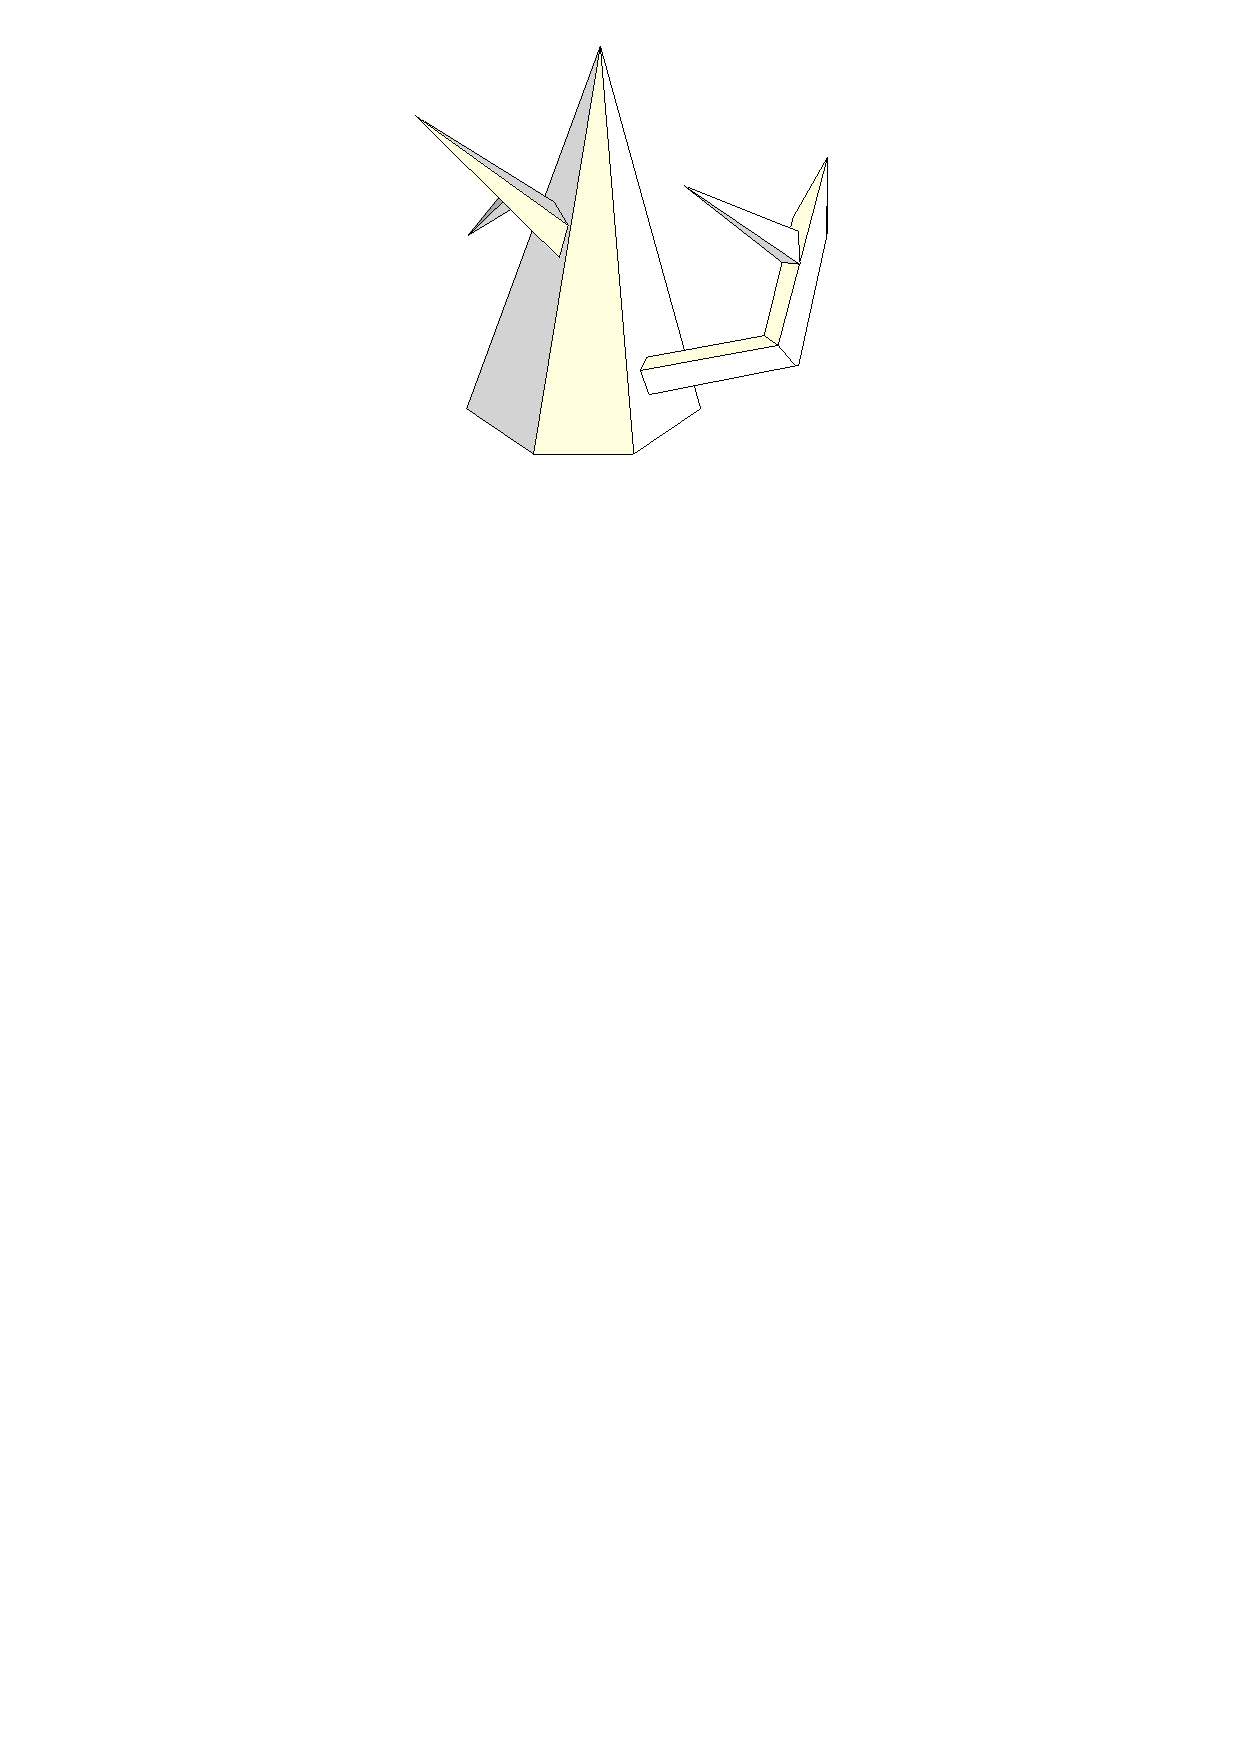
\includegraphics[width=.27\linewidth]{figs/spike3}%
    \hspace{.35in}
    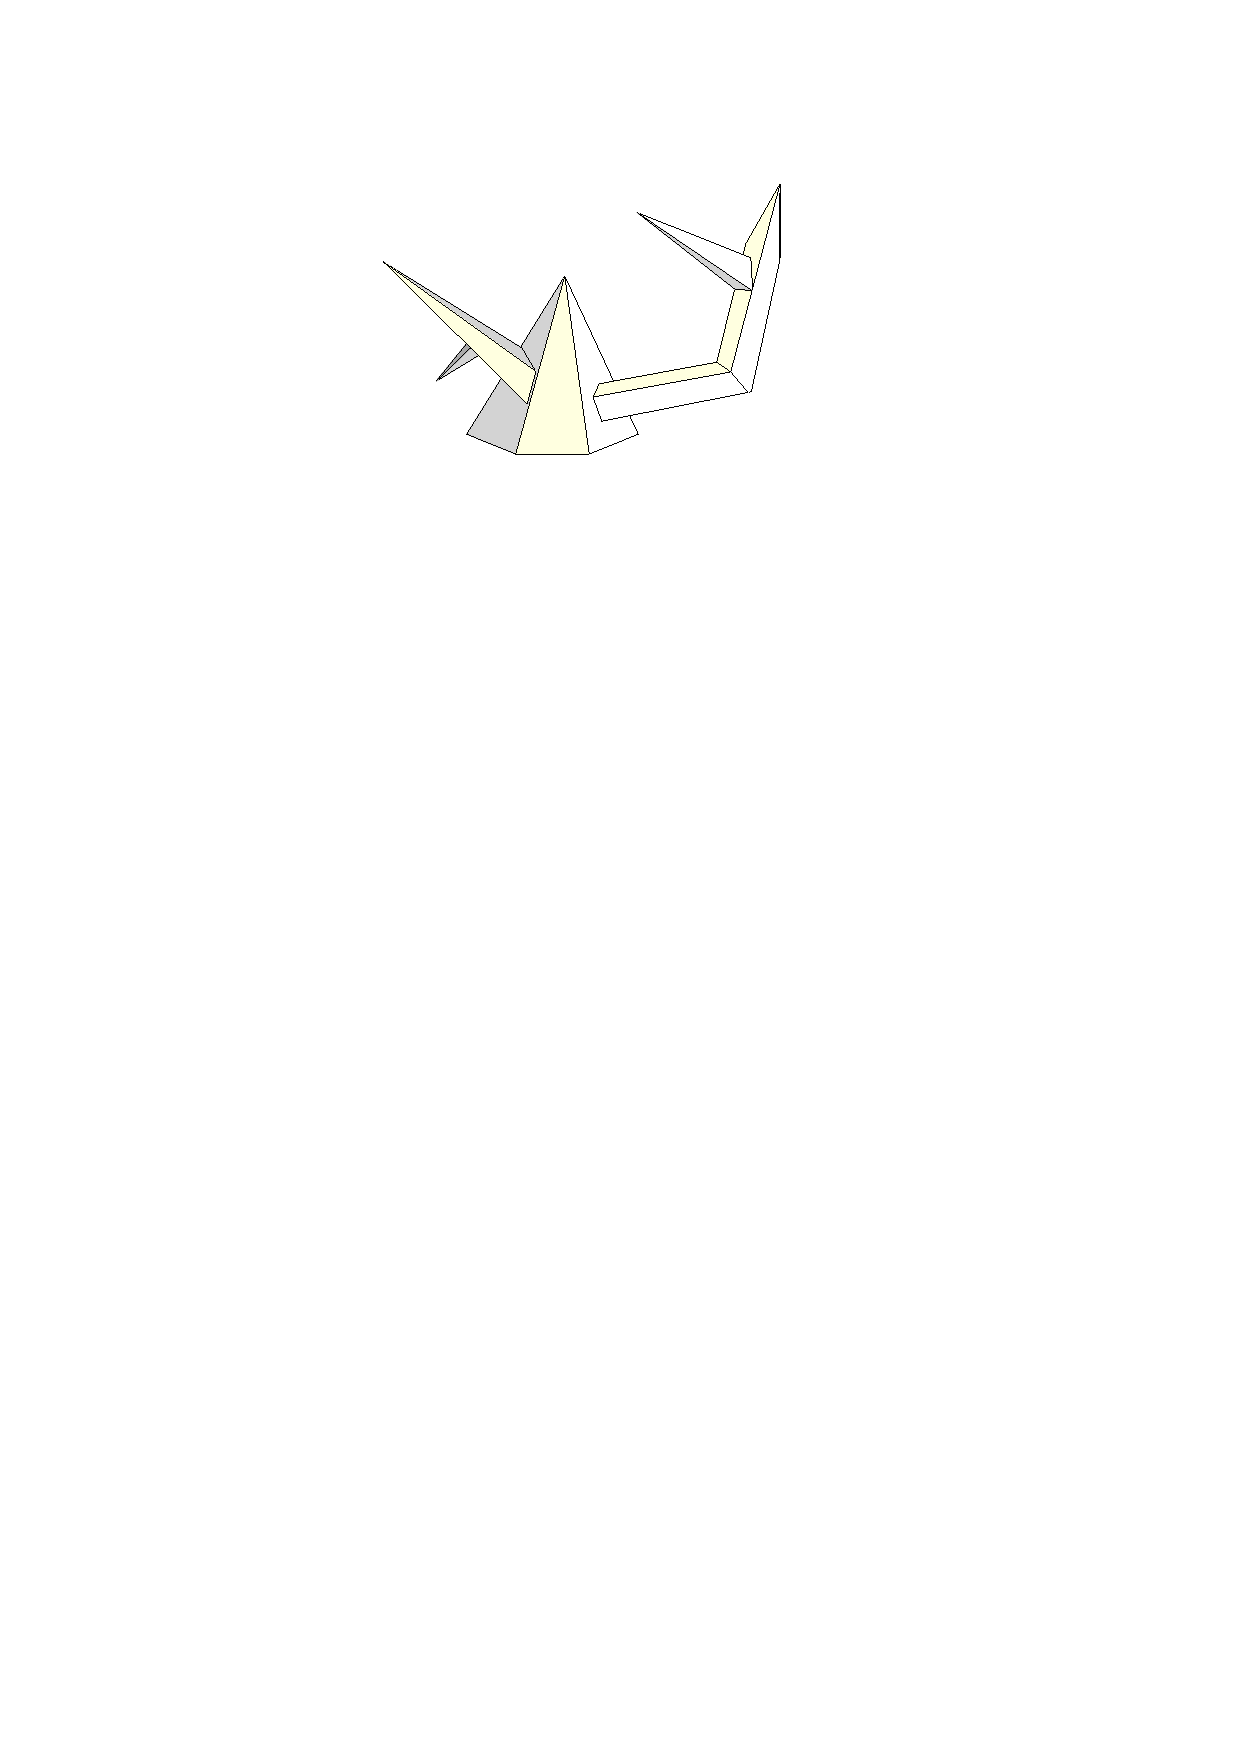
\includegraphics[width=.27\linewidth]{figs/spike4}%
    \hspace{.4in}
    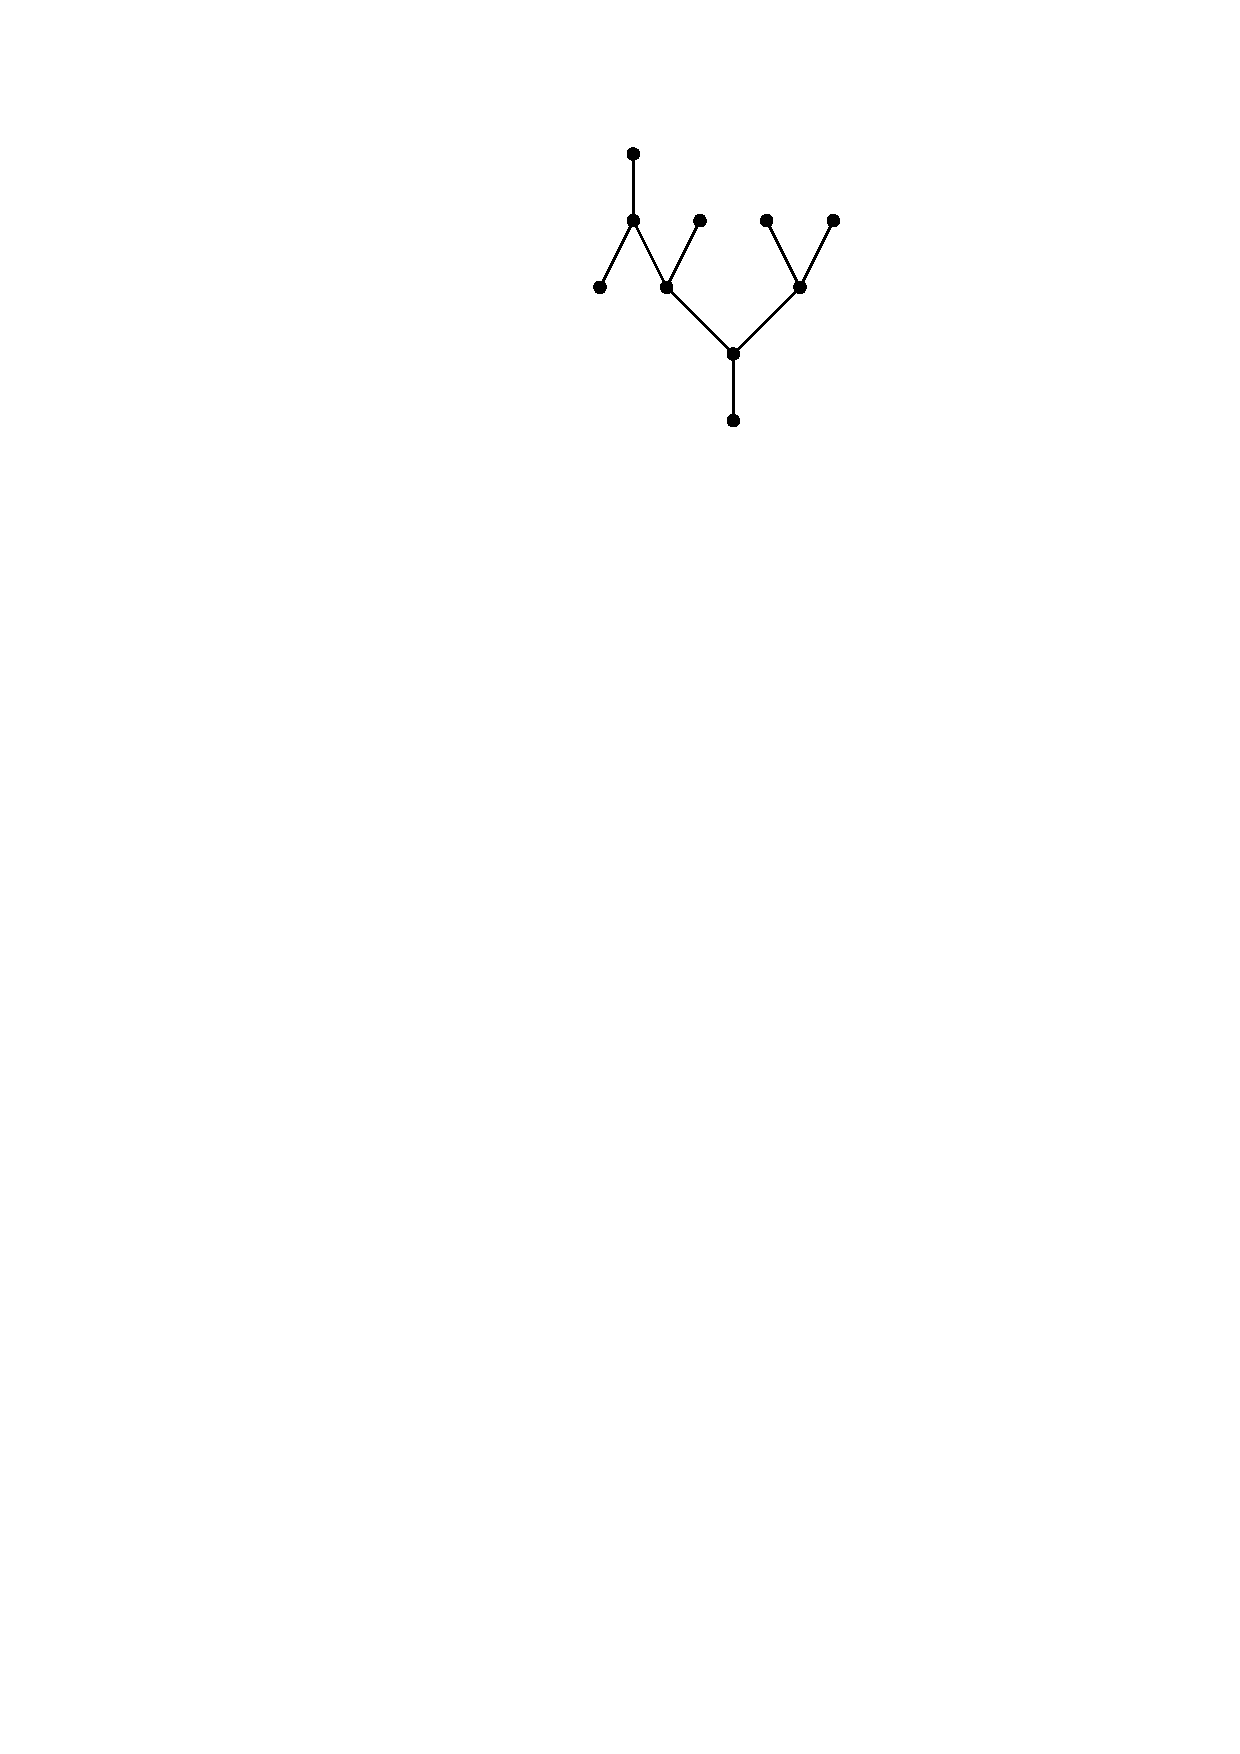
\includegraphics[width=.22\linewidth]{figs/spikeTree2}
    \caption{Two surfaces with different orderings of the maxima, but the same contour tree.}
    \label{fig:relative}
\end{figure}

\paragraph{The Issue of Sorting.}
As discussed above, the algorithm of Carr \etal \cite{csa-cctad-00} computes the contour 
tree by first constructing the join and split trees.  As vertices appear in sorted order 
in any root to leaf path in the join and split trees, and in any maxima to minima path 
in the contour tree, sorting the input vertices is a natural first step.  However, not 
all vertices from the input need to be sorted.  In particular, Chiang \etal 
\cite{cllr-sooscctmp-05} improved the running time by observing that as the join and 
split trees only consist of critical points, it suffices to only sort critical points.  
If a large fraction of the vertices appear in a single path in the join or split tree, 
then paying to sort all the critical points is unavoidable, and therefore in the worst 
case \cite{cllr-sooscctmp-05} is optimal.  However, if the trees are more balanced then 
sorting all critical points together can be very costly.  Specifically, the contour tree 
does not care about the relative ordering of vertices which do not have an 
ancestor-descendant relationship, and so this information does not need to be computed.
See \Fig{relative} for an example.

\begin{figure}[h]\centering
    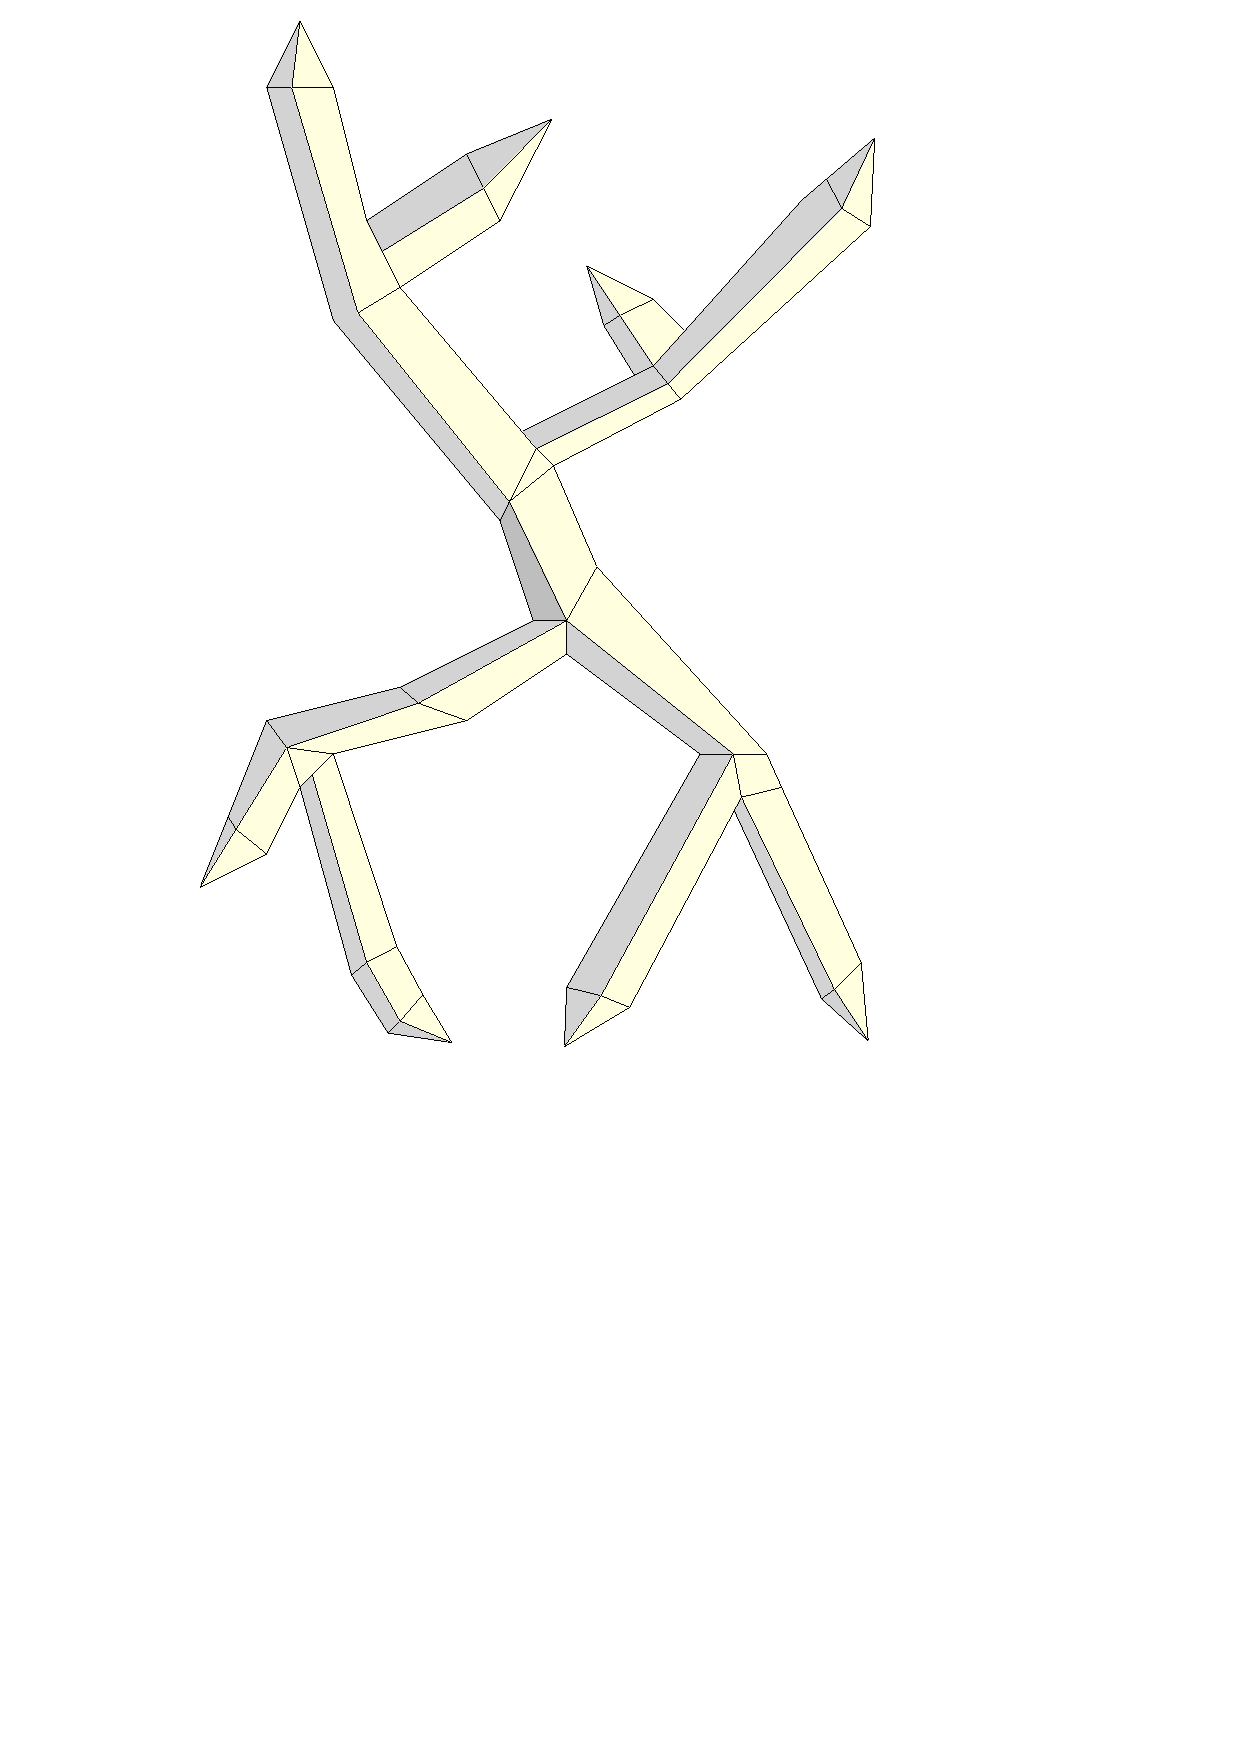
\includegraphics[width=.3\linewidth,height=.42\linewidth]{figs/shaded}%
    \hspace{.5in}
    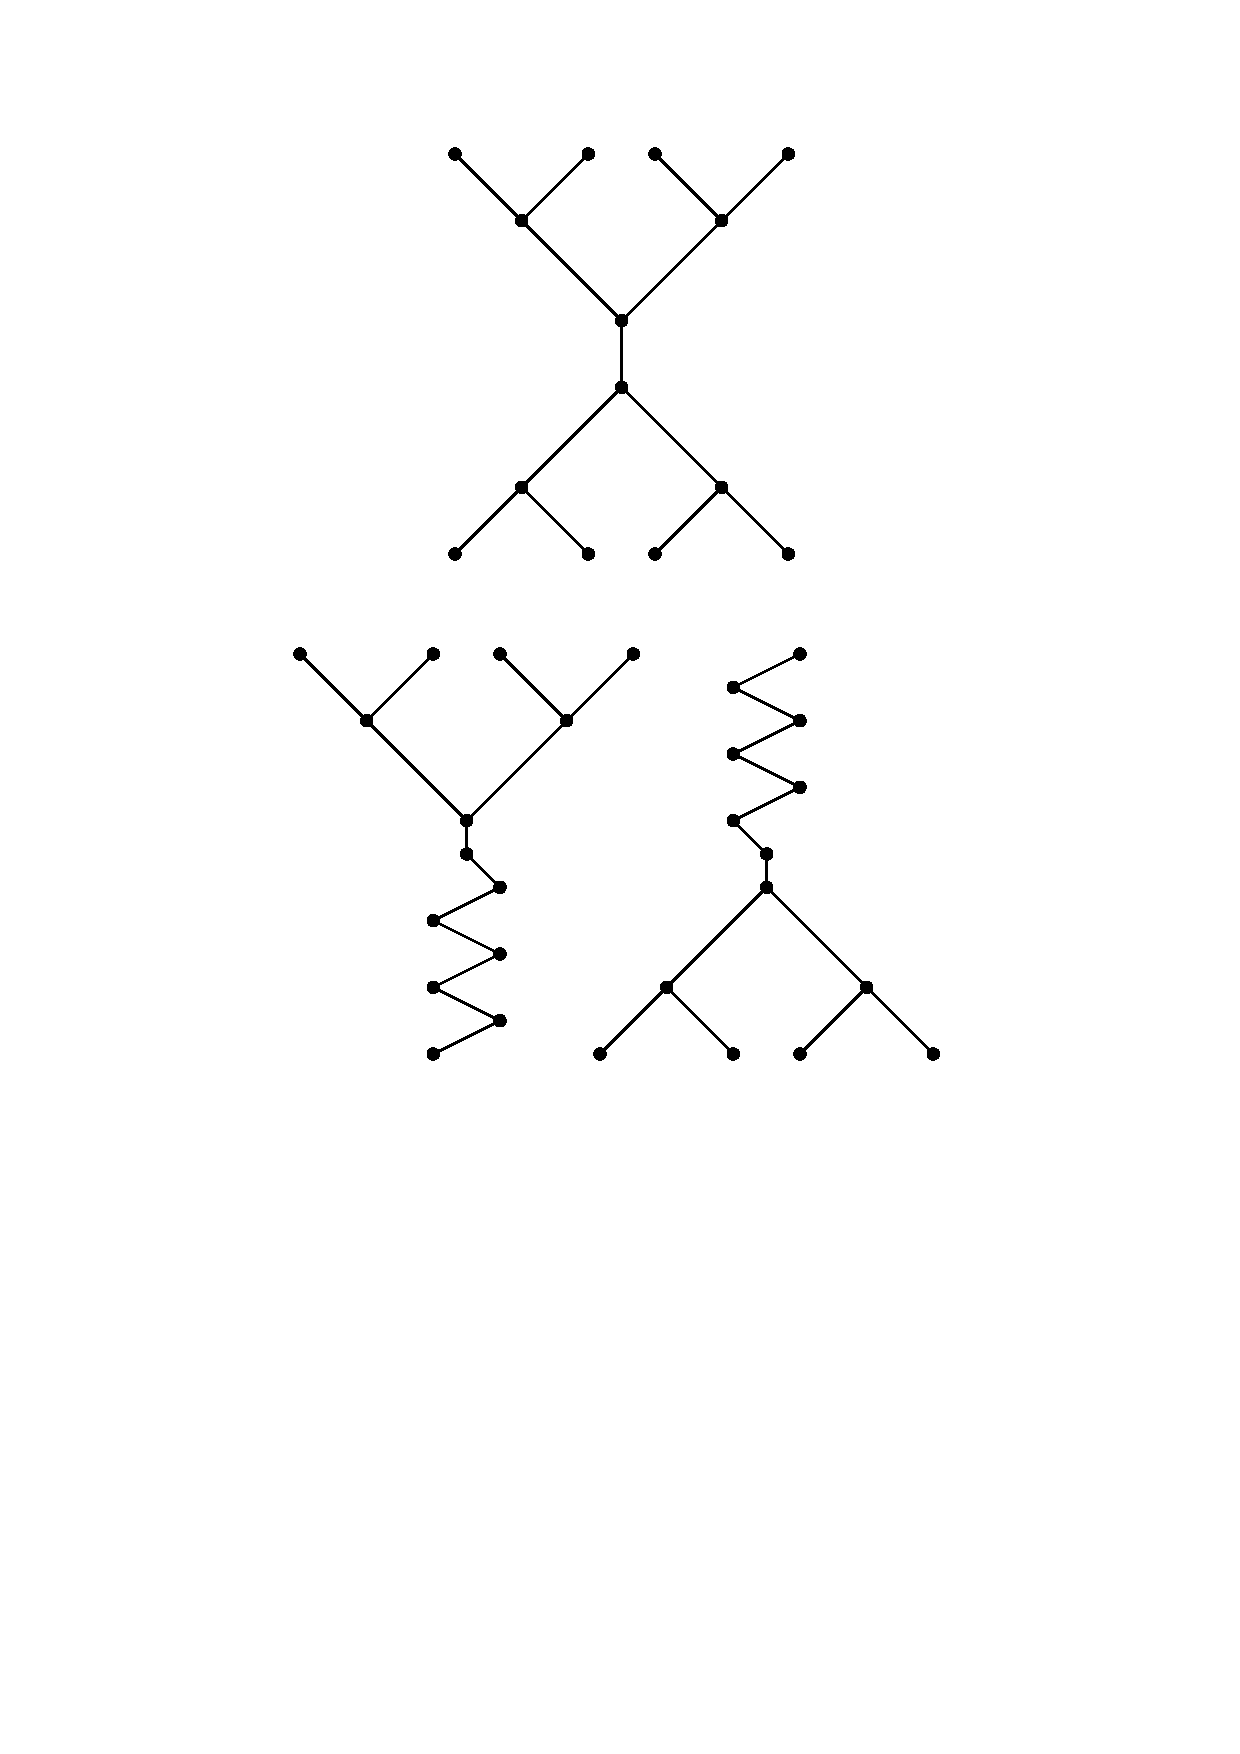
\includegraphics[width=.3\linewidth,height=.42\linewidth]{figs/trees2}
    \caption{On the left, a surface will a balanced contour tree, but whose merge and split trees have long tails.  
    On the right (in clockwise order from the top) the contour, split and merge trees.}
    \label{fig:sorting}
\end{figure}

\paragraph{Suboptimal Join and Split Trees.}
There is also a more fundamental problem with the now standard approach of first computing 
the join and split trees in order to compute the contour tree.  In particular, this approach 
can never lead to an algorithm that is optimal with respect to the shape of the contour tree.  
This is because it is possible to have join and split trees which are long and skinny (i.e. 
costly to compute) whereas the contour tree is balanced.  For example consider the case shown 
in \Fig{sorting}, where the mesh looks like two (thickened) balanced binary trees, one upside 
down, and joined at their roots.  In this case the contour tree is potentially cheap to 
compute as there is no long sorted path.  However, the join and split trees will have long 
sorted tails (consisting of the vertices in the bottom and top balanced trees, respectively), 
and therefore require $\Omega(n\log n)$ time to compute.

\subsection{Overview and Contribution}

\paragraph{Algorithm Overview.}
At a high level, the technique is rather simple.  Break the input manifold into nicely 
behaved pieces, compute the contour tree on each piece, and then stitch together the computed 
contour trees according to the cuts we made to break up the manifold.  Below we informally 
describe how this is accomplished.
\begin{compactitem}
 \item {\bf Raining to partition.}  To start with, pick an arbitrary maxima.  Now imagine 
 ``raining'' water down on the manifold from this maxima, i.e. mark all points which are reachable 
 by non-ascending paths from the maxima.  Let the boundary between wet and dry portions of the 
 manifold be called the interface (which may have different connected components).  
 Remove the wet submanifold, and invert the remaining pieces
 of the original manifold.  Now recursively rain in each one of these pieces, but rather than 
 picking an arbitrary maxima, start from the portion of the interface that cut that piece off.
 
 The benefit of this partitioning is that each resulting piece 
 is maxima dominant, i.e. there is a single maxima that has a non-ascending path to each point.  
 This implies the contour tree of this submanifold is the same as its split tree, or in other words 
 its contour tree is a rooted binary tree. 
 
 %
 \item {\bf Painting trees.}  For each maxima dominant piece we want to compute the split 
 tree without sorting all the vertices.  For conceptual ease lets first flip the submanifold 
 (i.e., it is now minima dominant and we compute the join tree).  Now arbitrarily pick a maxima 
 and spill paint from it, specifically color all edges and vertices of the mesh that are reachable 
 from the maxima by descending paths.  Now go to each other maxima and spill a different color, 
 but be aware that paints do not mix, i.e. if we reach a vertex that was previosly explored 
 by another color then we do not explore it.
 
 This procedure partitions the set of critical points into color classes.  Clearly each color 
 class is connected in the manifold.  Suppose each class was also connected in the join tree.  
 In this case we partitioned the join tree into a set of descending paths, each of which 
 can be constructed by sorting the critical points in a class.  Roughly speaking, 
 these paths can then be joined together by what amounts to doing a post-order traversal of the tree.
 However, we may not be so lucky and the color classes may not be connected in the 
 tree.  This turns out not to be a problem, but it requires proper data-structure use. 
%  
%  Now suppose we were lucky and the spilling of paint in the manifold corresponded with a paint 
%  spilling in the join tree, i.e. the color classes of the critical points partition the join 
%  tree into disjoint descending paths, each containing one leaf.   In this case 
%  we have partitioned the tree into branches, and so the tree can be formed by gluing these 
%  branches together.  Intuitively (i.e. not exactly true), if two branches glue together then 
%  it means there is a join vertex which got colored by the respective colors of each branch 
%  (only one of these colors actually explored the vertex in the mesh and this is the ``main'' 
%  branch you are gluing into).  Therefore, the tree can be constructed by starting at the leaf 
%  of the trunk (i.e. the branch with the global minima) and recursively building the subtrees 
%  while walking towards the root.  In other words we are building the tree by doing a post-order traversal.
%  Unfortunately, we may not be so lucky and the color classes may not appear contiguously in 
%  the tree.  In this case we can still build the tree in this leaf first fashion, but doing so 
%  efficiently requires the use of data-structures.
\end{compactitem}

\paragraph{Lower Bound Overview.}
In order to show that our algorithm for computing the join tree is optimal we consider paritioing the tree into disjoint 
descending paths, each containing a leaf.  It turns out that each such partition into paths, $P$, 
defines a lower bound of $\sum_{p\in P} |p|\log|p|$ for computing the contour tree, as you need to know the 
sorted order of the vertices along each path in order to determine the tree.
Specifically, we show that there is a set of at least $\Pi_{p_i\in P} (|p_i|-1)!$ distinct PL $2$-manifolds, 
all of which have the same defining mesh, and for which each sorted order of each group of saddles determines a different join tree.

The instance optimality of our algorithm then follows, as we also show that there is a particular path decomposition 
whose cost upper bounds our.  Specifically, we assign a weight to each node in the tree which is determined by 
the painting procedure described above (which represents the time it takes to process this node).  
The path decomposition then turns out to be the heavy-light path decomposition 
described by Sleator and Tarjan \cite{st-dsdt-83}, according to this weight function.
However, this decomposition is just the first step in the analysis, which 
requires further case analysis depending on the relative size of the length of each path 
and the weights of its vertices.

\paragraph{Our Contribution.}
Our contribution can be broken into three main aspects.  The first two are algorithmic.  Namely, 
first we describe a new linear time manifold partitioning scheme which breaks the manifold into 
``extremum'' dominant submanifolds.  
Second, we describe how to compute join trees optimally with respect to shape of the tree.
As the contour tree of each submanifold is (roughly) equal to its join tree, this leads to an 
optimal algorithm for the contour tree of the input manifold.  
Therefore, our third and final contribution is proving the optimality of this result, which 
requires a non-trivial amount of work, and uses techniques we believe to be of independent interest.

\paragraph{Organization.}
\Ben{To be Written}

\section{Contour tree basics} \label{sec:basics}

We detail the basic definitions about contour trees. The following is based on Chapter 6 of Carr's thesis \cite{c-tmi-04}.
Our input is a continuous PL function $f:\MM \mapsto \RR$, where $\MM$ is a fully triangulated simplicial complex in $\RR^d$. 
%All simplices are isomorphic to a standard $d$-dimensional simplex, except for specially designated \emph{boundary} simplices. 
\Sesh{Some mention of representation and data structures here.}
We use the standard assumption that $f$ is Morse (we explain later what this entails). 

Observe that $f:\MM \rightarrow \RR$ can be thought of as a $d$-dimensional simplicial complex living in $\RR^{d+1}$.
We can think of $f(x)$ as the ``height" of a point $x \in \MM$.
We will often omit $f$, and assume that $f$ is encoded in the representation of $\MM$.

\begin{definition} \label{def:level} The level set at value $h$ is the set $\{x \in \MM| f(x) = h\}$.
A contour is a maximal connected component of a level set. An $h$-contour is a contour where $f$-values are $h$.
\end{definition}

Note that a contour is itself a simplicial complex of one dimension lower, and is represented (in our algorithms) as such.
We let $\delta, \eps$ denote infinitesimals. Let $B_\eps(x)$ denote a ball of radius $\eps$ around $x$.

\begin{definition} \label{def:deg} The up-degree of $x \in \MM$ is the number of $(f(x) + \delta)$-contours that intersect $B_\eps(x)$
as $\delta, \eps \rightarrow 0^+$. The down-degree is the number of $(f(x) - \delta)$-contours that intersect $B_\eps(x)$
as $\delta, \eps \rightarrow 0^+$.
\end{definition}

The definition allows us to categorize points in $\MM$ depending on the local changes in topology.

\begin{definition} \label{def:points} A point $x \in \MM$ is categorized as follows.
\begin{asparaitem}
	\item Regular: Both up-degree and down-degrees are $1$.
	\item Maximum: Up-degree is $0$.
	\item Minimum: Down-degree is $0$.
	\item Join: Up-degree is strictly greater than $1$.
	\item Split: Down-degree is strictly greater than $1$.
\end{asparaitem}
Non-regular points are called \emph{critical}. Joins and splits are called \emph{saddles}.
Maxima and minima are called \emph{extrema}.
\end{definition}

\begin{remark}
 For two manifolds, at each saddle point either two contours join together or split apart, and hence the terminology.  In higher dimensions this may not be the case, however, it always holds that at a join or split vertex the topology of the level set changes, and hence such vertices are still 'critical'.  Note that determining which category each vertex falls into according to the above definition can be determined for all vertices simultaneously in linear time, as it is a local neighborhood condition.
\end{remark}



We will enforce a special constraint on boundaries, encapsulated in the following definition.

\begin{definition} \label{def:bound} $f$ is \emph{boundary critical} if the following holds.
Consider a boundary simplex $F$. All vertices of $F$ have the same function value. Furthermore, all
neighbors of $F$ not in $F$ either have all function values strictly greater or strictly less
than this value.
\end{definition}

\begin{remark}
Note that by assuming that our manifold is boundary critical, the vertices on a given boundary are either all maxima or all minima.  
Since all such vertices on a boundary component are in the same contour, we will abuse notation and refer to this entire set of vertices as a maxima (resp. minima).
In particular, we do not view this as a violation of the Morse condition on $f$, which requires distinct heights for critical points.
\end{remark}

We use $\cV$ to denote the set of critical points in $\MM$.
Because $f$ is piecewise-linear, all critical points are vertices in $\MM$. 
A value $h$ is called critical, if $f(x) = h$, for some $x \in \cV$. The Morse assumption
implies that all critical points have distinct values. A contour that involves a critical
point is also denoted as critical. Note that the vertices in a boundary face collectively behaves like an extremum.
Abusing notation, the term ``critical point", ``maxima", and ``minima" will include boundaries.
Critical values include these boundary values. By boundary criticality, all contours are themselves
represented as $d-1$-dimensional simplicial complexes.

\begin{definition} \label{def:equiv} Two contours $\psi$ and $\psi'$ are equivalent 
if the following holds. There exists an $f$-monotone path $p$ connecting a point in $\psi$ to $\psi'$,
such that no $x \in p$ belongs to a critical contour.
\end{definition}

These give the \emph{contour classes}. By continuity, a regular point is present on a single contour,
and we can partition the regular contours into these classes. Every such class maps to intervals
of the form $(f(x_i),f(x_j))$, where $x_i, x_j$ are critical points. Such a class is said
to be created at $x_i$ and destroyed at $x_j$. 

\begin{definition} \label{def:tree} The contour tree is the graph on vertex set $\cV$, where
edges are formed as follows. For every contour class that is created at $v_i$ and destroyed $v_j$,
there is an edge $(v_i,v_j)$. (Conventionally, edges are directed from higher function value to lower.)
\end{definition}

We denote the contour tree of $\MM$
by $\reeb(\MM) = \reeb(\MM,f)$. The corresponding node and edge sets are denoted as $\cV(\cdot)$ and $\cE(\cdot)$.
%
It is not immediately obvious that this graph is a tree, but the above definition is equivalent to that of the Reeb graph of $f:\MM \rightarrow \RR$ on $\MM$, and this is known to be a tree for PL functions defined over PL manifolds.  

\begin{remark}
Note that the contour tree as defined above contains vertices for all critical points, 
which differs slightly from the usual definition which only contains critical points corresponding to a change in the number of contours.  Specifically, if a vertex in the tree we defined has degree $2$ then only the topology of a contour is changing rather than the number of contour.  As such the standard contour tree can be computed from ours by a linear time pass to contract maximal degree 2 vertex paths.

For simplicity we will also make the standard assumption that vertices in the contour 
tree have degree at most $3$, i.e. there are no multi-saddles.
\end{remark}


We use a key theorem from \cite{c-tmi-04} (Theorem 6.6) that maps paths in $\cC(\MM)$ and $\MM$.


\begin{theorem} \label{thm:carr-path} For every path $P$ in $\MM$, there exists a path $Q$ in the contour tree corresponding
to the contours passing through points in $P$.
For every path $Q$ in the contour tree, there exists at least one path $P$ in $\MM$ through points present
in contours involving $Q$.
\end{theorem}

\begin{theorem} \label{thm:carr-mono} For every monotone path $P$ in $\MM$, there exists a monotone path $Q$ in the contour tree to which $P$
maps (as in the previous theorem), and vice versa.
\end{theorem}



\section{Divide and conquer through contour surgery} \label{sec:surgery}

{\bf The cutting operation:} We define a ``cut" operation on $f:\MM \rightarrow \RR$ that cuts along a regular contour to create
a new simplicial complex with an added boundary. Given contour $\phi$, this is constructing the simplicial complex $\MM \setminus \phi$. 
We will always enforce the condition that $\phi$ never passes through a vertex of $\MM$.
Again, we use $\eps$ for an infinitesimally small value. We denote $\phi^+$ (resp. $\phi^-$) to be
the contour at value $f(\phi) + \eps$ (resp. $f(\phi) - \eps$), which is at distance $\eps$
from $\phi$. 

An $h$-contour is achieved by intersecting $\MM$ with the hyperplane $x_{d+1} = h$ and taking a connected component. (Think of the $d+1$-dimension
as height.) Given some point $x$
on an $h$-contour $\phi$ (with some simplex that $x$ is present in), we can walk along $\MM$ from $x$ and determine $\phi$.
We can ``cut" along $\phi$ to get a new (possibly) disconnected simplicial complex $\MM'$. This is achieved
by splitting every facet $F$ that $\phi$ intersects into an ``upper" facet and ``lower" facet. Algorithmically,
we cut facet $F$ with $\phi^+$ and take everything above $\phi^+$ in $F$ to make the upper facet. Analogously, we cut with $\phi^-$ to get the lower facet.
The facets are then triangulated to ensure that they are all simplices.
Given that $\phi$ cannot cut a boundary and all non-boundary facets
have constant size, we omit the algorithmic description for this process. We only note that this
creates the two new boundaries $\phi^+$ and $\phi^-$, and we maintain the property of constant $f$-value at a boundary.
This new simplicial complex is denoted by $\cut(\phi,\MM)$.
This can be constructed in time linear in $|\phi|$.

%We denote this new manifold by $\cut(\phi,\MM)$, and the new boundaries by $\phi^+$ and $\phi^-$.
%Abusing notation, we use $\cut(\phi,\MM)$
%for a set $\Psi$ of contours to mean the manifold obtained by cutting along all contours in $\Phi$.


\ignore{
\medskip
\fbox{
\begin{minipage}{0.9\textwidth}
{\bf $\cut(\phi,\MM)$}

\smallskip
\begin{asparaenum}
%	\item Insert the vertices of $\phi$ in $\MM$.
	\item For every edge $e$ that intersects $\phi$ at point $x$: add edges $(e,x^+)$ and $(e,x^-)$
	where $x^+$ (resp. $x^-$) is infinitesimally above (resp. below) $x$.
	\item Take a point $x$ (resp. $y$) on $e$ at distance $\eps$ above (resp. below) $\phi$.
	\item Let $\phi_x$ be the contour through $x$, and analogously define $\phi_y$. Insert a vertex
	at each intersection point of these contours with edges of $\MM$. Add  
	\item Delete the edges between $\phi_x$ and $\phi_y$.
\end{asparaenum}
\end{minipage}}

\medskip
This results in a new boundary critical simplicial complex. There are two new disjoint
boundary simplices added. The manifold may be disconnected. 
}

We now describe a high-level approach to construct $\reeb(\MM)$.

\medskip
\fbox{
\begin{minipage}{0.9\textwidth}
{\bf $\surgery(\MM,\phi)$}

\smallskip
\begin{asparaenum}
	\item Let $\MM' = \cut(\phi,\MM)$.
	\item Construct $\reeb(\MM')$ and let $A, B$ be the nodes corresponding to the new boundaries created
	in $\MM'$. (One is a minima and the other is maxima.)
	\item Since $A, B$ are leaves, they each have unique neighbors $A'$ and $B'$, respectively. Insert
	edge $(A',B')$ and delete $A, B$ to obtain $\reeb(\MM)$.
\end{asparaenum}
\end{minipage}}

\medskip
\begin{theorem} \label{thm:surgery} For any regular contour $\phi$, the output of $\surgery(\MM,\phi)$ is $\reeb(\MM)$.
\end{theorem}

The main theorem is a direct consequence of the following lemma. 

\begin{lemma} \label{lem:cut} Consider a regular contour $\phi$ contained in a contour class (of an edge of $\reeb(\MM))$
$(u,v)$ and denote $\MM' = \cut(\phi,\MM)$. Then $\cV(\reeb(\MM')) = \{\phi^+,\phi^-\} \cup \cV(\MM)$
and $\cE(\reeb(\MM')) = \{(u,\phi^+),(\phi^-,v)\} \cup (\cE(\MM) \setminus (u,v))$.
\end{lemma}

\begin{proof} The contours of $\MM'$ are exactly the contours of $\MM$ with $\phi^+$ and $\phi^-$, without $\phi$.
All new vertices created in $\MM'$ are present on $\phi^+$ and $\phi^-$. That proves the first part.

Any contour class in $\MM'$ (edge in $\cC(\MM')$) that does not involve $\phi^+$ or $\phi^-$ is also
a contour class in $\MM$. Furthermore, a maximal contour class satisfying these properties is also
maximal in $\MM$. So all edges of $\cC(\MM')$ that do not involve $\phi^+$ or $\phi^-$ are edges of $\cC(\MM)$.
Analogously, every edge of $\cC(\MM)$ not involving $\phi$ is an edge of $\cC(\MM')$.

Consider the contour class corresponding to edge $(u,v)$ of $\cC(\MM)$. There is a natural ordering
of the contours by function value, ranging from $f(u)$ to $f(v)$. All contours in this class ``above" $\phi$
form a maximal contour class in $\MM'$, represented by edge $(u,\phi^+)$. Analogously, there is another
contour class represented by edge $(\phi^-,v)$. We have now accounted for all contours in $\cC(\MM')$,
completing the proof.
\end{proof}

A useful corollary of this lemma shows that a contour actually splits the simplicial complex into
two disconnected complices.

\begin{theorem} \label{thm:jordan} $\cut(\phi,\MM)$ consists of two
disconnected simplicial complices.
\end{theorem}

\begin{proof} Denote (as in \Lem{cut}) the edge containing $\phi$ to be $(u,v)$. Suppose for contradiction that there is a path between vertices $u$ and $v$
in $\MM' = \cut(\phi,\MM)$. By \Thm{carr-path}, there is a path in $\cC(\MM')$ between $u$ and $v$. Since $\phi^+$ and $\phi^-$
are leaves in $\cC(\MM')$, this path obviously cannot use edges incident to them. By \Lem{cut},
all the edges of this path are in $\cE(\cC(\MM)) \setminus (u,v)$. So we get a cycle in $\cC(\MM)$, a contradiction.
To show that there are exactly two connected components in $\cut(\phi,\MM)$, it suffices
to see that $\cC(\MM')$ has two connected components (by \Lem{cut}) and apply \Thm{carr-path}.
\end{proof}

\section{Raining to partition $\MM$} \label{sec:rain}

In this section, we describe a linear time procedure that partitions $\MM$ into special
\emph{extremum dominant} simplicial complices.

\begin{definition} \label{def:dom} A simplicial complex is \emph{minimum dominant} if there exists
a minimum $x$ such that every non-minimal \emph{vertex} in the manifold has a decreasing path to $x$.
Analogously define \emph{maximum dominant}. 
\end{definition}

The first aspect of the partitioning is ``raining". Start at some point $x \in \MM$ and imagine rain at $x$.
The water will flow downwards along descending paths and ``wet" all the points encountered. Note that this procedure considers all points
of the manifold, not just vertices.

\begin{definition} \label{def:wet} Fix $\MM$ and $x \in \MM$. The set of points $y \in \MM$ such that there is a non-ascending path from $x$ to $y$
is denoted by $\wet(x,\MM)$ (which is in turn is represented as a simplicial complex). A point $z$ is at the \emph{interface} of $\wet(x,\MM)$ if every neighborhood of $z$
has non-trivial intersection with $\wet(x,\MM)$.
\end{definition}

The following claim gives a description of the interface. While its meaning is quite intuitive, the proof is tedious.

\begin{claim} \label{clm:inter} For any $x$, the interface of $\wet(x,\MM)$ is a set of contours,
each containing a join vertex.
\end{claim}

\begin{proof} If $p \in \wet(x,\MM)$, all the points in any contour containing $p$ are also in $\wet(x,\MM)$.
 (Follow the non-ascending path to from $x$ to $p$ and then walk along the contour.) The converse is also true,
 so $\wet(x,\MM)$ contains entire contours.

Let $\eps, \delta$ be sufficiently small as usual. Fix some $y$ at the interface.
Note that $y \in \wet(x,\MM)$. (Otherwise, $B_\eps(y)$ is dry.)
The points in $B_\eps(y)$ that lie below $y$ have a descending path from $y$ and hence must be wet.
There must also be a dry point in $B_\eps(y)$ that is above $y$, and hence,
there exists a dry, regular $(f(y)+\delta)$-contour $\phi$ intersecting $B_\eps(y)$.

Let $\Gamma_y$ be the contour containing $y$.  Suppose for contradiction
that $\forall p \in \Gamma_y$, $p$ has up-degree $1$ (see \Def{deg}). Consider the non-ascending path from $x$ to $y$ and let $z$
be the first point of $\Gamma_y$ encountered. There exists a wet, regular $(f(y) + \delta)$-contour $\psi$ 
intersecting $B_\eps(z)$. Now, walk from $z$ to $y$ along $\Gamma_y$. If all points $w$ in this walk
have up-degree $1$, then $\psi$ is the unique $f(y)+\delta$-contour
intersecting $B_\eps(w)$. This would imply that $\phi = \psi$, contradicting the fact that $\psi$ is wet
and $\phi$ is dry.

Therefore, there must exist a join vertex $w$ in $\Gamma_y$, such that $B_\eps(w)$ intersects
both $\phi$ and $\psi$. As $\delta, \eps \rightarrow 0^+$, the limit of $\phi$ (which is dry)
lies in $\Gamma_y$ (which is wet). 
Hence this limit gives a contour of the interface containing the join $w$.
\end{proof}

\ignore{
\begin{proof} If $y \in \wet(x,\MM)$, all the points in any contour containing $y$ are also in $\wet(x,\MM)$.
 (Follow the non-ascending path to from $x$ to $y$ and then walk along the contour.)
 First observe that any point which in the interface must be wet.  Second, for $y \in \wet(x,\MM)$, all the points in any contour containing $y$ are also in $\wet(x,\MM)$, 
 as one can follow the non-ascending path to $y$ and then walk along the contour.
 
 So let $y$ be a point in the interface. 
 
 However, since $y$ is in the interface, it is also wet.  Therefore for any contour $\phi$ which contains $y$, for any arbitrarily small $\eps$ there is 
 a wet point which lies above $\phi$ and has a descending path of length at most $\eps$ to $\phi$.
 This implies there is some contour which lies just 
 above $y$ which is wet.  So any contour $\phi$ containing $y$ has two contours which lie just above it, one which is dry, and one which is wet.  
 This can only happen if $\phi$ contains a merge vertex, because otherwise all contours which lie just above would be in the same L-homotopy equivalence class and so by 
 \Clm{mono}, if one is wet, all below it are wet.
 
 By similar logic one can argue that of the two contours through a given merge vertex at most one can contain interface points other than the merge vertex, 
 and that if one of the contours does contain such interface points, then the entire contour consists of interface points.
\end{proof}
}


Note that $\wet(x,\MM)$ (and its interface) can be computed in time linear in the size of the wet simplicial complex.
We perform a non-ascending search from $x$. Any facet $F$ of $\MM$ encountered is partially (if not entirely) in $\wet(x,\MM)$.
This portion is determined by cutting $F$ along the interface. Since the interface is a contour, this is equivalent
to cutting $F$ by a hyperplane. All these operations can be performed to output $\wet(x,\MM)$ in time linear in $|\wet(x,\MM)|$.


% \begin{proof} If $y \in \wet(x,\MM)$, but not in the interface, then any contour containing $y$ is also in $\wet(x,\MM)$.
% So consider a point $y$ in the interface. We argue that all points in a contour $\phi$ containing $y$
% are also in the interface. If such a contour is regular, we can find a contour just above it that
% is also wet. 
% 
% If two contours intersect, the intersection point $y$ is critical. We can argue that the only
% way to reach $y$ from a descending path is reach one of the contours and then follow it to get to $y$.
% But that would imply the existence of another critical point on this contour, violating the Morse condition.
% 
% Let us argue that $y$ is a merge vertex. Consider the descending path from $x$ to $y$. The final edge
% that reaches $y$ is obviously all wet, and is an increasing edge from $y$. Consider an opposite increasing
% edge. Take two point in these edges that are infinitesimally higher than $y$ and show that the contours
% through them as disjoint. So $y$ is a merge.
% \end{proof}

We define a simple \lift{} operation on the interface contours. Consider such a contour $\phi$ containing
a merge vertex $y$. Take any dry increasing edge incident to $y$, and pick the point $z$ on this edge at height
$f(y) + \delta$. Let $\lift(\phi)$ be the unique contour through the regular point $z$. Note that $\lift(\phi)$ is dry.

\begin{claim} \label{clm:cut-int} Let $\phi$ be an interface contour. Then $\cut(\MM,\lift(\phi))$
results in two disjoint simplicial complices, one consisting entirely of dry points.
\end{claim}

\begin{proof} By \Thm{jordan}, $\cut(\MM,\lift(\phi))$ results in two disjoint simplicial complices. Let $\NN$ be the complex containing
the point $x$ (the argument in $\wet(x,\MM)$), and let $\NN'$ be the other complex. 
Any path from $x$ to $\NN'$ must intersect $\lift(\phi)$, which is dry. Hence $\NN'$ is dry.
%
%
%If there exists a wet point $z$ in $\NN'$, then there exists a descending path from $x$ to $z$. 
%As $x$ is in $\NN$ and $z$ is in $\NN'$, again by the Jordan Curve Theorem this path must intersect $\phi$, 
%contradicting the fact that $\phi$ is dry.
\end{proof}


\begin{figure}[h]\centering
    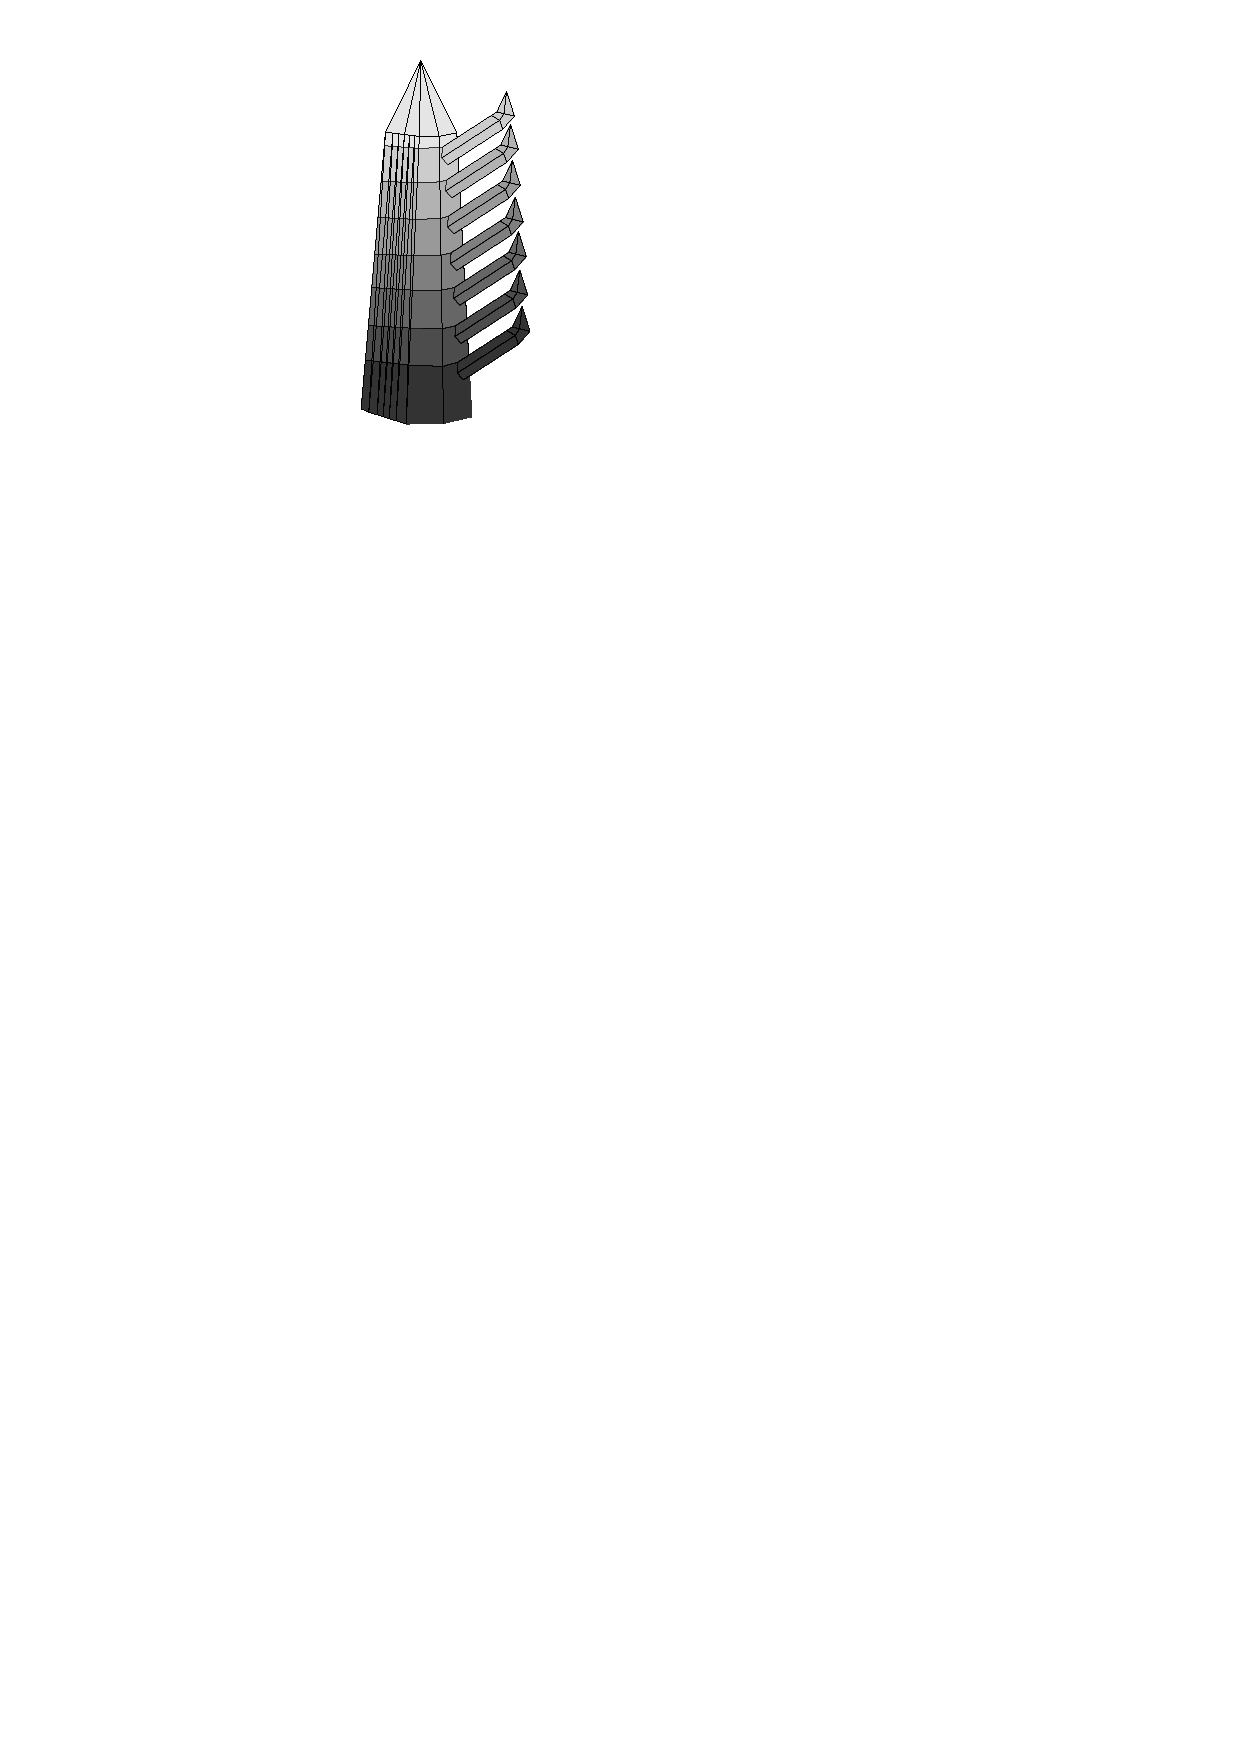
\includegraphics[width=.18\linewidth,height=.35\linewidth]{figs/orderGray1}%
    \hspace{.8in}
    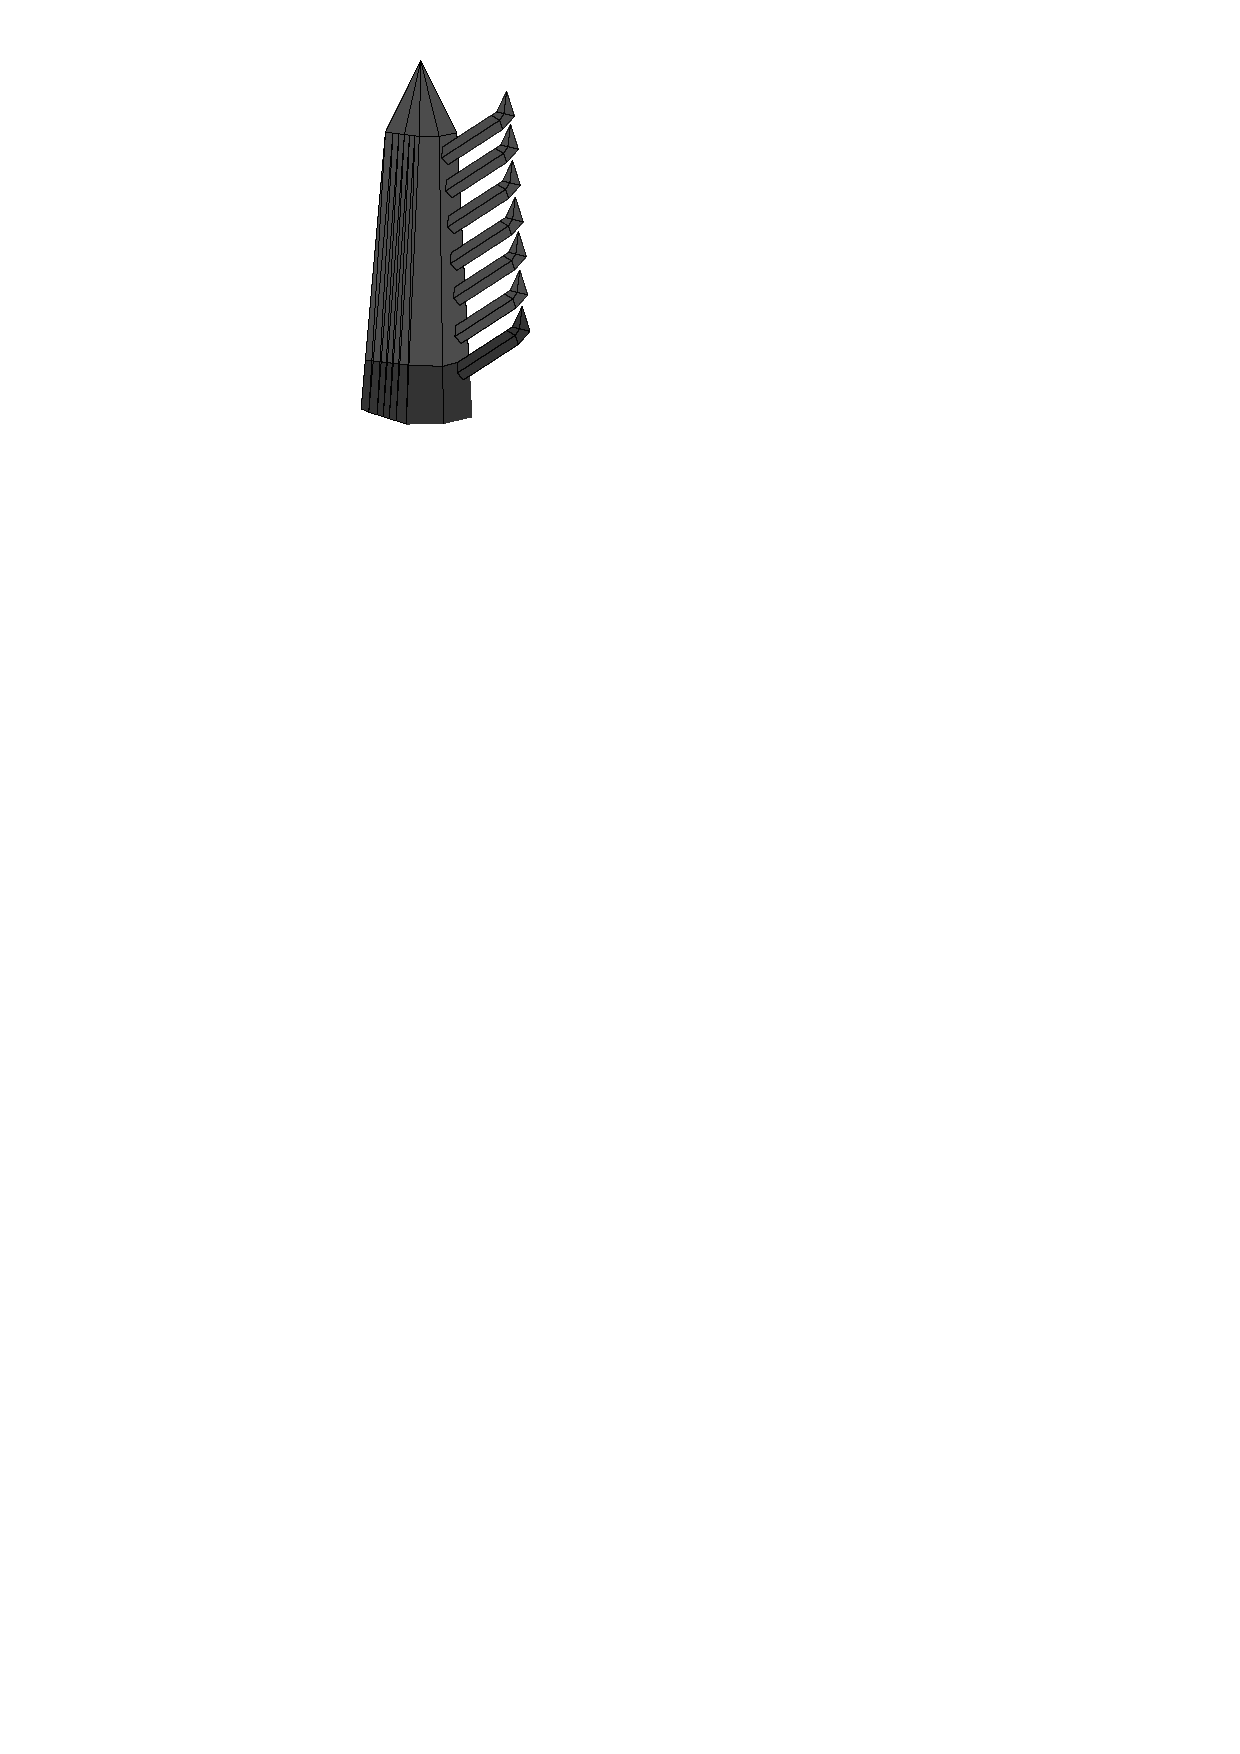
\includegraphics[width=.18\linewidth,height=.35\linewidth]{figs/orderGray2}
    \caption{On left, downward paint spilling only (each shade of gray represents a different color), producing a grid.  On right, flipping the direction of paint spilling.}
    \label{fig:order}
\end{figure}

We describe the main partitioning procedure that cuts a simplicial complex $\NN$ into extremum
dominant complices. It takes an additional input of a maximum $x$. To initialize,
we begin with $\NN$ set to $\MM$ and $x$ as an arbitrary maximum. One of the critical aspects
of the procedure is that the rain alternately flows downwards and upwards, 
since otherwise faces may be cut a super constant number of times (see \Fig{order}).
In other words, when
we start, rain flows downwards. In each recursive call, the direction of rain is switched to the 
opposite direction. While one can implement $\rain$ this way, it is conceptually easier
to think of \emph{inverting} a complex $\NN'$ when a recursive call is made. Inversion
is easily achieved by just negating the height values. (From a running time standpoint, it suffices
to maintain a single bit associated with $\NN'$ that determines whether heights are inverted or not.)
We can now let rain flow downwards, as it usually does in our world.

%
%We critically perform
%an \emph{inversion} step, which is simply achieved by negating
%
\medskip
\fbox{
\begin{minipage}{0.9\textwidth}
{\bf $\rain(x,\NN)$}

\smallskip
\begin{compactenum}
	\item Determine interface of $\wet(x,\NN)$. 
	\item If the interface is empty, simply output $\NN$. Otherwise, denote the contours by $\phi_1, \phi_2, \ldots, \phi_k$ and set $\phi'_i = \lift(\phi_i)$.
	\item Initialize $\NN_1 = \NN$.
	\item For $i$ from $1$ to $k$: 
	\begin{compactenum}
		\item Construct $\cut(\phi'_i,\NN_i)$, consisting of dry complex $\LL_i$ and remainder $\NN_{i+1}$.
		\item Let the newly created boundary of $\LL_i$ be $B_i$. Invert $\LL_i$ so that $B_i$ is a maximum. Recursively
		call $\rain(B_i,\LL_i)$.
	\end{compactenum}
	\item Output $\NN_{k+1}$ together with any complices output by recursive calls.
\end{compactenum}
\end{minipage}}

\medskip
For convenience, denote the total output of $\rain(x,\MM)$ by $\MM_1, \MM_2, \ldots, \MM_r$.
We first argue the correctness of $\rain$.

\begin{lemma} \label{lem:rain-1} Each output $\MM_i$ is extremum dominant.
\end{lemma}

\begin{proof} Consider a call to $\rain(x,\NN)$. If the interface is empty, then all of $\NN$
is in $\wet(x,\NN)$, so $\NN$ is trivially extremum dominant. So suppose the interface
is non-empty and consists of $\phi_1, \phi_2, \ldots, \phi_k$ (as denoted in the procedure).
By repeated applications of \Clm{cut-int}, $\NN_{k+1}$ contains $\wet(x,\MM)$. 
Consider $\wet(x,\NN_{k+1})$. The interface must exactly be $\phi_1, \phi_2, \ldots, \phi_k$.
So the only dry vertices are those in the boundaries $B_1, B_2, \ldots, B_k$. But these
boundaries are maxima.
\end{proof}

Focus on $\rain(x,\MM)$. As $\rain$ proceeds, new facets/simplices are created because of repeated cutting. Indeed, any facet $F$
in any simplicial complex $\NN$ that is recursively invoked, is achieved by cutting facet $F'$ in $\MM$.
The key to the running time of $\rain(x,\MM)$ is bounding the number of newly created facets, for which we have the following lemma.

\begin{lemma}\label{lem:new-verts}
A facet $F \in \MM$ is cut at most once during $\rain(x,\MM)$.
\end{lemma}
\begin{proof} All notation here follows that in the pseudocode of $\rain$.
First, by \Thm{jordan}, all the pieces on which $\rain$ is invoked are disjoint.
Second, all recursive calls are made on dry complices.

Consider the first time that $F$ is cut, say, during the call to $\rain(x,\NN)$.
Specifically, say this happens when $\cut(\phi'_i,\NN_i)$ is constructed. 
So $F$ is cut by some hyperplane into lower and upper portions (which are then triangulated).
Since the cut is infinitesimally above an interface, the lower portion is basically wet.
It can never be part of $\LL_1, \LL_2, \ldots$, which go into recursive calls. This portion
is in $\NN_{k+1}$. The upper portion/facet (call it $U$) is in $\LL_i$. Note that the lower
boundary of $U$ is in the boundary $B_i$. Since a recursive call is made to $\rain(B_i,\LL_i)$
(and $\LL_i$ is inverted), $U$ becomes wet. Hence, $U$ will not be cut subsequently.
All in all, $F$ is cut at most once.
\ignore{
As the number of edges is $O(n)$, arguing that there is at most one boundary vertex created along any given edge will imply the claim.
Consider some edge $e$ and take the first time a boundary vertex is created in $e$.
This happens when some contour $\phi$ intersects $e$. On applying $\cut(\NN,\lift(\phi))$,
consider the dry manifold $\LL$ and wet manifold $\MM$ constructed. The edge $e$ is split into two parts, the dry and wet part.
The wet part is in $\MM$ and will never be involved in any recursive call.

The dry part of $e$ (call it $e'$) needs to be considered.
A boundary vertex $v$ (an new endpoint of $e$) is created, which is part of the boundary $B$ in $\LL$,
such that $\rain(B,\LL)$ is called to the inverted $\LL$. In this call, since the water starts from $v$,
all of $e'$ becomes wet. So there is no further interface contour that can intersect this portion of $e'$.
}
\end{proof}


\begin{theorem} \label{thm:rain-time} The total running time of $\rain(x,\MM)$ is $O(|\MM|)$.
\end{theorem}

\begin{proof} The operations performed are the raining and cutting. We can bound this by the total
complexities of the wet complices and the new boundaries created. No facet is ever wet twice,
and by \Lem{new-verts}, the total number of facets that every appear is $O(|\MM|)$. This also 
bounds the complexities of the boundaries created.
\end{proof}

\ignore{
As each original vertex in $\NN$ appears in only one of the sub-manifolds output by $\rain(x,\NN)$, we have the following corollary.

\begin{corollary}
The total size of a sub-manifolds output by $\rain(x,\MM)$ is $O(n)$.
\end{corollary}

\begin{corollary} \label{cor:rain-time} The total running time of $\rain(x,\MM)$ is $O(n)$.
\end{corollary}

\begin{proof} Consider some invocation to $\rain(x,\MM)$. The only non-trivial work done in $\rain$ is by the calls to $\wet$.
We know that each invocation to $\wet$ runs in time linear 
to the portion of the manifold which is wet (including the new boundary vertices created).  
As the output of $\rain$ is precisely the distinct sub-manifolds wet by each distinct call to $\wet$, the claim follows.
\end{proof}
 
%Consider one of the manifolds $\MM_i$ output by $\rain$.  This manifold has a set of boundary maxima/minima that are the result 
%of cutting along interface contours.  For each such contour there is exactly one other output manifold $\MM_j$ for which 
%the contour appears as a boundary maxima/minima. 
}



\begin{claim} \label{clm:rain-reeb} Given $\reeb(\MM_1), \reeb(\MM_2), \ldots, \reeb(\MM_r)$, 
%be the output of $\rain(x,\MM)$. Suppose that for each reeb graph we know its corresponding vertex in the Manifold Ordering Tree. 
$\reeb(\MM)$ can be constructed in $O(|\MM|)$ time.
\end{claim}

\begin{proof} Consider the tree of recursive calls in $\rain(x,\MM)$, with each node
labeled with some $\MM_i$.
%
%There is a natural tree ordering defined over these manifolds where the 
%root corresponds the first manifold that was wet when we rained from $x$, and its children correspond to the recursive calls 
%(i.e. where we rained from the interface contours of the first raining).  Call this the \emph{Manifold Ordering Tree}.
%$\rain$ can easily be modified to also output this tree (without affecting the asymptotic running time).  
Walk through this tree in a leaf first ordering.  Each time we visit a node we connect its contour tree to the 
contour tree of its children in the tree using the $\surgery$ procedure. 
Each $\surgery$ call is constant time, and the total time is the size of the recursion tree.
%
%
%This takes $O(n)$ time overall by \Lem{new-verts} and since $\surgery$ takes constant time (given the appropriate vertices in each reeb graph).  The correctness follows by induction and  \Lem{surgery}.
\end{proof}


\section{Contour trees of extremum dominant manifolds} \label{sec:paint}

The previous section allows us to restrict attention to extremum dominant manifolds.
We will orient so that the extremum in question is always a \emph{minimum}.
We will fix such a simplicial complex $\MM$, with the dominant minimum $m^*$. 
The set of non-dominant minima is denoted by $M$.
For vertex $v$, we use $\MM^+_v$ to denote the simplicial complex obtained by only
keeping vertices $u$ such that $f(u) > f(v)$. Analogously, define $\MM^-_v$. Note that $\MM^+_v$ may contain
numerous connected components. 

The main theorem of this section asserts that the contours trees of minimum dominant manifolds have a simple description.
The exact statement will require some definitions and notation.
We required the notions of \emph{join} and \emph{split} trees, as given by~\cite{csa-cctad-00}.
Conventially, all edges are directed from higher to lower function value. We will use the terminology
``parent" for an adjacent node that is higher. Because of the orientation, a node
may have multiple parents.
%We first explain what these trees are.

\begin{definition} \label{join} The join tree $\cJ(\MM)$ of $\MM$ is built on vertex set $V(\MM)$.
The directed edge $(u,v)$ is present when $u$ is the smallest valued vertex in a connected component of $\MM^+_v$
\emph{and} $v$ is connected to this component (in $\MM$). The split tree $\cS(\MM)$ is obtained
by looking at $\MM^-_v$ (or alternately, by taking the join tree of the inversion of $\MM$). 
\end{definition}


Some basic facts about these trees. 
%Note that unlike the contour tree, all vertices in $\MM$ are present in $\cJ(\MM)$ and $\cS(\MM)$. 
All outdegrees in $\cJ(\MM)$ are at most $1$, all indegree $2$ vertices are joins, all leaves are maxima,
and the global minimum is the root. All indegrees in $\cS(\MM)$ are at most $1$, all outdegree $2$
vertices are splits, leaves are minima, and the global maximum is the root.
The key observation is that $\cS(\MM)$ is trivial for a minimum dominant $\MM$.

\begin{lemma} \label{lem:split} $\cS(\MM)$ consists of:
\begin{asparaitem}
	\item A single path (in sorted order) with all vertices except non-dominant minima.
	\item Each non-dominant minimum is attached to a unique split (which is adjacent to it).
\end{asparaitem}
\end{lemma}

\begin{proof} It suffices to prove that each split $v$ has one child that is just a leaf, which
is a non-dominant minimum.  Specifically, any minimum is a leaf in $\cS(\MM)$ and thereby attached to a split, 
which implies that if we removed all non-dominant minima, we must end up with a path, as asserted above.

Consider a split $v$. For sufficiently small $\eps, \delta$, there are exactly two $(f(v) - \delta)$-contours
$\phi$ and $\psi$ intersecting $B_\eps(v)$. Both of these are regular contours. There must be a non-ascending
path from $v$ to the dominant minimum $m^*$. Consider the first edge (necessarily decreasing from $v$)
on this path. It must intersect one of the $(f(v) - \delta)$-contours, say $\phi$. By \Thm{jordan}, $\cut(\MM,\phi)$ has
two connected components, with one (call it $\LL$) having $\phi^-$ as a boundary maximum. This complex
contains $m^*$ as the non-ascending path intersects $\phi$ only once. Let the other
component be called $\MM'$.

Consider $\cut(\MM',\psi)$ with connected component $\NN$ having $\psi^-$ as a boundary. $\NN$
does not contain $m^*$, so any path from the interior of $\NN$ to $m^*$ must intersect the boundary $\psi^-$.
But the latter is a maximum in $\NN$, so there can be no non-ascending path from the interior to $m^*$.
Since $\MM$ is overall minimum dominant, the interior of $\NN$ can only contain a single vertex $w$, a non-dominant
minimum.

The split $v$ has two children in $\cS(\MM)$, one in $\NN$ and one in $\LL$. The child in $\NN$ can only
be the non-dominant minimum $w$, which is a leaf. 
\end{proof}

It is convenient to denote the non-dominant minima as $m_1, m_2, \ldots, m_k$
and the corresponding splits (as given by the lemma above) as $s_1, s_2, \ldots, s_k$. 

To prove our main theorem, we use the merging procedure from~\cite{csa-cctad-00} that constructs the contour tree
from the join and split trees. 
It actually construsts the \emph{augmented contour tree} $\cA(\MM)$, which
is the contour tree with regular points inserted into the edges. 
Consider tree $T$ with vertex $v$ of in and outdegree at most $1$.
\emph{Erasing} $v$ from $T$ is the following operation: if $v$ is a leaf, just delete $v$. Otherwise, smooth $v$ out
(delete $v$ and connect its neighbors by an edge). This tree is denoted by $T \ominus v$.


\medskip
\fbox{
\begin{minipage}{0.9\textwidth}
{\bf $\merge(\cJ(\MM),\cS(\MM))$}

\smallskip
\begin{compactenum}
	\item Set $\cJ = \cJ(\MM)$ and $\cS = \cS(\MM)$.
	\item Denote $v$ as \emph{candidate} if sum of indegree of $v$ in $\cJ$ and outdegree of $v$ in $\cS$ is $1$. 
	\item Add all candidates to queue.
	\item While candidate queue is non-empty: 
	\begin{compactenum}
		\item Let $v$ be head of queue. If $v$ is leaf in $\cJ$, consider its edge in $\cJ$. Otherwise
		consider its edge in $\cS$. In either case, denote the edge by $(v,w)$.
		\item Insert $(v,w)$ in $\cA(\MM)$. 
		\item Set $\cJ = \cJ \ominus v$ and $\cS = \cS \ominus v$. Enqueue any new candidates.
	\end{compactenum}
	\item Smooth out all regular vertices in $\cA(\MM)$ to get $\cC(\MM)$.
\end{compactenum}
\end{minipage}}

\medskip

\begin{definition} 
\label{def:criticalJoin}
The critical join tree $\jc(\MM)$ is built on the set $V'$ of all
critical points other than the non-dominant minima. 
The directed edge $(u,v)$ is present when $u$ is the smallest valued vertex in $V'$ in a connected component of $\MM^+_v$
and $v$ is connected to this component (in $\MM$). 
\end{definition}


\begin{theorem} \label{thm:contour-tree} Let $\MM$ have a dominant minimum. 
The contour tree $\cC(\MM)$ consists of all edges $\{(s_i, m_i)\}$ and $\jc(\MM)$.
\end{theorem}


\begin{proof} We first show that $\cA(\MM)$ is $\cJ(\MM) \ominus \{m_i\}$ with edges $\{(s_i,m_i)\}$.
We have flexibility in choosing the order of processing in $\merge$. We first put the non-dominant
maxima $m_1, \ldots, m_k$ into the queue. As these are processed, the edges $\{(s_i,m_i)\}$ are inserted 
into $\cA(\MM)$. Once all the $m_i$'s are erased, $\cS$ becomes a path, so all outdegrees are at most $1$.
The join tree is now $\cJ(\MM) \ominus \{m_i\}$. We can now process $\cJ$ leaf by leaf, and all
edges of $\cJ$ are inserted into $\cA(\MM)$.

Note that $\cC(\MM)$ is obtained by smoothing out all regular points from $\cA(\MM)$. Smoothing out regular
points from $\cJ(\MM) \ominus \{m_i\}$ exactly yields the edges described in the theorem.
\end{proof}

\section{Painting to compute contour trees}

The main algorithmic contribution is a new algorithm for computing join trees of any triangulated simplicial
complex $\MM$.

%
%As part of the initialization, we determine
%all critical points in $\MM$. For any vertex $v$, we can look at $f(v) \pm \delta$-contours 
%in $f|_{B_\eps(v)}$ to determine the up and down degrees. This determines the criticality (and type)
%of $v$. This requires $O(|\MM|)$ time, since every facet is looked at proportional to the number of its
%vertices.

{\bf Painting:} The central tool is a notion 
of \emph{painting} $\MM$. Initially associate a color with each maximum. Imagine there being a large
can of paint of a distinct color at each maxima $x$. We will spill different paint from each maximum and watch it flow down.
This is analogous to the raining in the previous section, but paint is a much more viscous liquid.
\emph{So paint only flows down edges, and it does not color the interior of facets.} Furthermore, paints
do not mix, so every edge of $\MM$ gets a unique color. This process (and indeed the entire algorithm)
works purely on the 1-skeleton of $\MM$, which is just a graph.
%
\begin{definition} \label{def:paint} Let the 1-skeleton of $\MM$ have edge set $E$ and maxima $X$.
A  \emph{painting} of $\MM$ is a map $\chi:X \cup E \mapsto [|X|]$ with the following property. 
 Consider an edge $e$. There exists a descending path from some maximum $x$ to $e$
	consisting of edges in $E$, such that all edges along this path have the same color as $x$. 

An \emph{initial} painting has the additional property that the restriction $\chi:X \mapsto [|X|]$ is a bijection.
\end{definition}
%
%Paintings are not unique. It is straightforward to construct an initial painting of $\MM$ in $O(|\MM|)$ time, 
%using a descending BFS from each maximum that does not explore previously colored edges. 
%As the algorithm proceeds, the bijection property will not hold, though we always maintain a valid painting.

A painting only colors edges, not vertices. We associate certain
sets of colors with vertices.

\begin{definition} \label{def:color-set} Fix a painting $\chi$ and vertex $v$.
\begin{asparaitem}
	 \item An \emph{up-star} of $v$ is the set of edges that all connected to a fixed component of $\MM^+_v$.
	 \item A vertex $v$ is \emph{touched by color $c$} if $x$ is incident to a $c$-colored
	 edge with $v$ at the lower endpoint. For $v$, $\col(v)$ is the set of colors that touch $v$.
	 \item A color $c \in \col(v)$ \emph{fully touches} $v$ if all edges in an up-star are colored $v$.
\end{asparaitem}
\end{definition}

Each non-maxima $v$ participates in at least $1$ and at most $2$ up-stars (the latter iff
$v$ is a join).

\ignore{
Abusing notation, we say a contour $\phi$ is of color $c$ if all edges that intersect $\phi$ have color $c$.

\begin{definition} \label{def:color-full} Consider vertex $v$. An \emph{up-star} of $v$ is the set 
of edges that all connected to a fixed component of $\MM^+_v$. 
%and let $\phi$ be a $(f(v)+\delta)$-contour in
%$f|_{B_\eps(v)}$. If $\phi$ is monochromatic of color $c$, then $v$ is \emph{fully touched by $c$}. The set of colors
%that fully touch $v$ is denoted $\fcol(v)$.
\end{definition}

%Note that $\fcol(v)$ has size at most $2$, by the Morse condition. 
Note that $\col(v)$ 
%and $\fcol(v)$ can
be initially determined in $O(|\MM|)$ time, by a simple linear scan.
}


\subsection{The overall approach and the data structures} \label{sec:struct}

We give an informal description of the algorithm, which might motivate the data structures.

Our algorithm incrementally builds $\jc(\MM)$ from the leaves (maxima) to the root (dominant minimum). 
Let us focus on an initial painting, where the colors have 1-1 correspondence with the maxima.
Consider two sibling leaves $\ell_1, \ell_2$ and their common parent $v$. The leaves are maxima,
and $v$ is a join that ``merges" $\ell_1, \ell_2$. A nice mental picture is given when $\MM$ is 2-dimensional.
In that case, there are ``mounds" corresponding to each $\ell_1$ and $\ell_2$ that merge
at a valley $v$. Suppose this was the entire input, and $\ell_1$ was colored blue and $\ell_2$ was colored red. 
Both the mounds are colored completely blue or red, while $v$ is touched by both colors.
Moreover, each up-star of $v$ (one connecting to each mound) is fully colored. So this
indicates that $v$ joins the blue maxima and red maxima in $\jc(\MM)$.

This is precisely how we hope to exploit the information in the painting. We prove later that
when some join $v$ has both up-stars fully colored, the corresponding maxima (of those colors) are exactly
the parents of $v$ in $\jc(\MM)$. To proceed further, we ``merge" the colors red and blue into a new color, purple. In other words,
we replace all red and blue edges by purple edges. This indicates that the red and blue maxima have been
handled. Imagine flattening the red and blue mounds until reaching $v$, so that the former join $v$
is now a new maxima. Suppose purple paint was poured from $v$. In terms of $\jc(\MM)$, this
is equivalent to removing leaves $\ell_1$ and $\ell_2$, making $v$ a new leaf.
Alternately, $\jc(\MM)$ has been constructed up to $v$, and it remains to determine $v$'s parent.

Of course, things are more complicated when there are other mounds. There may be a yellow mound,
corresponding to $\ell_3$ that joins with the blue mound higher up (at vertex $u$). In $\jc(\MM)$, $\ell_2$ and $\ell_3$
are sibling leaves, and $\ell_1$ is a sibling of some ancestor of these leaves. So we cannot
merge red and blue, until yellow and blue merge. Naturally, we use priority queues to handle this issue.
We know that $u$ must also be (fully) touched by blue. So all critical vertices touched by blue
are put into a priority queue keyed by height, and vertices are handled in that order.

What happens when finally blue and red join at $v$? We merge the two colors, but now have
blue and red queues of critical vertices. We also need to merge the priority queues
to get a consistent painting. And that decides the use of \emph{binomial heaps} to store the
critical points of one color. Merges can be done in logarithmic time, the same time
required for deletes.

In this discussion, we have ignored a somewhat annoying problem. Up-stars of critical vertices
may actually be touched by numerous colors, not just one as we assumed above. A simple solution
would be to insert vertices into heaps corresponding to all colors touching it. But there could
be super-constant numbers of copies of a vertex, and handling all these copies would lead
to extra overhead. We show that it suffices to simply put each vertex $v$ into at most two heaps,
one for each up-star. We are guaranteed that when $v$ needs to be processed, its up-stars
automatically have one color, because of all the color merges that previously occured.

With this preamble, we are ready to discuss our data structures. We discuss all the initializations
in the next section.

\medskip
\noindent
{\bf The binomial heaps $\touch(c)$:} For each color $c$, $\touch(c)$ is a subset of vertices touched by $c$,
This is stored as a \emph{binomial max-heap} keyed by vertex heights. Abusing notation, $\touch(c)$ refers
both to the set and the data structure used to store it.

%We initialize as follows. For each critical vertex $v$ and from each of its up-stars, we pick an arbitrary color $c$ touching $v$. 
%We insert $v$ into $T(c)$. Observe that $v$ participates in at least $1$ and at most $2$ heaps.
%

\medskip
\noindent
{\bf The union-find data structure on colors:} We will repeatedly perform unions
of classes of colors, and this will be maintained as a standard union-find data structure.
For any color $c$, $\rep(c)$ denotes the representative of its class. 

\medskip
\noindent
{\bf The stack $\st$:} This consists of non-extremal critical points, with monotonically increasing
heights as we go from the base to the head.
\ignore{
Each point $x \in \st$ has an associated subset of $\col(x)$, denoted $\mcol(x)$.
Both $\mcol(x)$ and its complement are stored as hash table. So lookups, inserts, and deletes
are in these sets are all constant time operations. The stack is guaranteed to satisfy 
the following invariants.
\begin{asparaitem}
	\item For every $x \in \st$: For every $c \in \mcol(x)$, $x$ is the highest element
	in $T(c)$. Furthermore, $c = \rep(c)$.
	\item Consider $x, y \in \st$ such that $y$ was pushed on $x$. There exists $c \in \col(x) \setminus
	\mcol(x)$ such that $x$ is not highest in $T(c)$ but $y$ is highest in $T(c)$.
\end{asparaitem}
}

\medskip
\noindent
{\bf Attachment vertex $\h(c)$:} For each color $c$, we maintain a critical point $\h(c)$ of this color.
We will maintain the guarantee that the portion of the contour tree above (and including) $\h(c)$ has already been constructed.
%This is initialized to the maximum corresponding to $c$.

\ignore{
\medskip
As the algorithm proceeds, it is convenient to imagine
it maintaining a set of contours $\Phi = \{\phi_1, \phi_2, \ldots, \phi_k\}$, which are contained
in incomparable edges of $\cC(\MM)$. Suppose we cut $\MM$ by each of these contours, and took
the simplicial complex $\NN$ where $\phi^-_i$'s are all boundary maxima. The algorithm will
have already determined the contour trees of the simplicial complices
where $\phi^+_i$ is a boundary maxima. 

During this process, various colors will be \emph{merged}. This involves merging the respective $T(c)$'s and
updating the union-find data structure. The only operation performed on $T(c)$'s are delete-max and merge.
No new vertex is ever inserted into the heaps. As colors merge, the initial painting is obviously modified.
But it would be too expensive to explicitly update colors. So the new painting is given by $\rep(c)$,
while we only have access to the original painting. By union-find bounds, this only adds an $\alpha(|\MM|)$
overhead to the data structure operations. The new coloring is guaranteed to be a painting of $\NN$.

%While this is the intuitive viewpoint, we describe how this information is actually maintained.
The vertices $\{\h(\rep(c))\}$ represent the set of contours $\Phi$. In terms of the contour tree, 
we have already constructed the contour trees rooted at each $h(\rep(c))$. This is trivially true at the initialization,
when each $h(c)$ is a maximum. One can now treat each $h(\rep(c))$ as a maximum, corresponding to (a possibly new) color $\rep(c)$.
To reduce confusion between the original painting and the new colors, we will assume that $\col(v)$ and $\fcol(v)$
are as given by the original painting. 
}
	
\subsection{The algorithm} \label{sec:algo}

We formally describe the algorithm below. 
We require a technical definition of \emph{ripe} vertices.


\begin{definition} \label{def:ripe} A vertex $v$ is \emph{ripe} if: for all $c \in \col(v)$, $v$
is present in $T(\rep(c))$ and is also highest vertex in the heap. 
%Also, for all $c \in \col(v) \setminus \fcol(v)$, $T(\rep(c))$ is empty.
\end{definition} 

\medskip
\fbox{
\begin{minipage}{0.9\textwidth}
{\bf $\init(\MM)$}

\smallskip
\begin{compactenum}
	\item Construct an initial painting of $\MM$ using a descending BFS from maxima that does not explore previously colored edges.
	\item Determine all critical points in $\MM$. For each $v$, look at $(f(v) \pm \delta)$-contours in $f|_{B_\eps(v)}$ 
	to determine the up and down degrees. 
	\item Mark each critical $v$ as unprocessed.
	\item For each critical $v$ and each up-star, pick arbitrary color $c$ touching $v$. Insert $v$ into $T(c)$.
	\item Initialize $\rep(c) = c$ and set $\h(c)$ to be the unique maximum colored $c$.
\end{compactenum}
\end{minipage}}


\medskip
\fbox{
\begin{minipage}{0.9\textwidth}
{\bf $\build(\MM)$}

\smallskip
\begin{compactenum}
	\item Run $\init(\MM)$.
	\item While there are unprocessed critical points:
	\begin{compactenum}
		\item Run $\update(\st)$. Pop $\st$ to get $h$.
		\item Let $\cur(h) = \{\rep(c) | c \in \col(h)\}$.
		\item For all $c' \in \cur(h)$:
		\begin{compactenum}
			\item Add edge $(\h(c'),h)$ to $\jc(\MM)$.
			\item Delete $h$ from $T(c')$ (if present).
		\end{compactenum}
	\item Merge heaps $\{T(c') | c' \in \cur(h)\}$.
	\item Take union of $\cur(h)$ and denote resulting color by $\widehat{c}$.
	\item Set $\h(\widehat{c}) = h$ and mark $h$ as processed.
	\end{compactenum}
\end{compactenum}
\end{minipage}}

\medskip
\fbox{
\begin{minipage}{0.9\textwidth}
{\bf $\update(\st)$}

\smallskip
\begin{compactenum}
	\item If $K$ is empty, push arbitrary unprocessed critical point $v$.
	\item Let $h$ be head of $\st$.
	\item While $h$ is not ripe:
	\begin{compactenum}
		\item Find $c \in \col(h)$ such that $h$ is not present or not the highest in $T(\rep(c))$.
		\item Push the highest of $T(\rep(c))$ onto $\st$, and update head $h$.
	\end{compactenum}
\end{compactenum}
\end{minipage}}

\bigskip

A few simple facts:
\begin{asparaitem}
	\item At all times, the colors form a valid painting.
	\item Each vertex is present in at most $2$ heaps. After processing, it is removed from all heaps.
	\item After $v$ is processed, all edges incident to $v$ have the same color (technically, same representative). 
	\item When $\update(\st)$ terminates, the head $h$ is ripe. 
\end{asparaitem}


\medskip
\ignore{	
	Suppose $\mcol(h) = \{c\}$ (so $h$ is split). 
	\begin{compactenum}
		\item Connect $h$ (in $\reeb(\MM)$) to $\h(c)$ and the unique minimum corresponding to split $h$. 
		\item Delete $h$ from $T(c)$, set $\h(c) = h$.
		\item End procedure.
	\end{compactenum}
	\item Let $\mcol(h) = \{c_1, c_2\}$ (so $h$ is merge).
	\item Connect $h$ in $\reeb(\MM)$ to $\h(c_1)$ and $\h(c_2)$.
	\item Delete all copies of $h$ from $T(c_1)$ and $T(c_2)$.
	\item Perform union of colors $c_1$ and $c_2$ (denote merged color as $c$). Merge heaps
	to get $T(c) = T(c_1) \cup T(c_2)$.
	\item Set $\h(c) = h$.	

We state the primary invariant below.
First, some notation. For any $v$, let $\psi^-_v$ denote the $(f(v)-\delta)$-contour intersecting
$B_\eps(v)$. If there are two such contours (so $v$ is a split), choose the one that contains
the dominant minimum. The \emph{palette} $\pal$ is the set of colors currently used,
which is $\{T(\rep(c)) | c \in |X|\}$.


Observe that $\build(\MM)$ loops over all unprocessed critical point.
The invariant is true at the starting point of each such iteration.

\medskip
\textbf{Invariant:} 
\begin{compactenum}
	\item For every $c \in \pal$, the subtree of $\cJ(\MM)$ rooted at $\h(c)$ has been constructed.
	\item Fix $c \in \pal$. Consider the set $S$ of maxima of $\MM$ in the subtree of $\cJ(\MM)$ rooted at $\h(c)$.
	Then $\rep(c) = \bigcup_{s \in S} \chi(s)$.
	\item Let $\Psi = \{\psi^-_{\h(c)} | c \in \pal\}$. The coloring given by $\rep(\cdot)$
	is a valid painting of $\cut(\MM,\Psi)$, where $\psi^-_{\h(c)}$ has color $c$.
\end{compactenum}

\medskip
It is easy to see that the invariant is true at the very beginning of the algorithm.
Each $\h(c)$ is simply the maximum colored with $c$, and we have a valid painting of $\MM$.
}


\section{Proving correctness} \label{sec:correct}

\ignore{
\begin{claim} \label{clm:process} Assume the invariant. Any vertex with a non-increasing path to some $\h(c)$
for $c \in \pal$ has been processed.
\end{claim}

\begin{proof} This is a direct consequence of \Thm{carr-mono}, which relates monotone paths in $\MM$ to $\cC(\MM)$.
Since the subtree of $\cJ(\MM)$ (which is basically the subtree of $\cC(\MM)$) rooted at $\h(c)$ 
has been found, all vertices in this subtree must be processed. These are all the vertices with non-increasing paths
to $\h(c)$ in $\cC(\MM)$, which by \Thm{carr-mono} is the same as those in $\cC(\MM)$.
\end{proof}
}

Our main workhorse is the following technical lemma. 

\begin{lemma} \label{lem:full} Suppose vertex $v$ is connected to a component of $\MM^+_v$
by edge $e$ of color $c$. Either all edges in $\MM^+_v$ are colored $c$, or there
exists critical vertex $w \in \MM^+_v$ fully touched by $c$ and touched by another color.
%
%and take $(f(v)+\delta)$-contour $\phi$ intersecting
%$B_\eps(v)$. Suppose the edges incident to $v$ intersecting $\phi$ do not have the same color. For any such
%color $c$, there exists a critical vertex $w$ strictly higher than $v$ such that $c \in \fcol(v)$.
\end{lemma}

\begin{proof} Since $e$ has color $c$,
there must exist vertices in $\MM^+_v$ touched by $c$. Consider the highest
vertex $w$ in $\MM^+_v$ that is touched by $c$ and some other color. If no such vertex exists,
this means all edges incident the a vertex touched by $c$ are colored $c$. By walking through
$\MM^+_v$, we deduce that all edges are colored $c$. 

So assume $w$ exists. Take the $(f(w)+\delta)$-contour $\phi$ that intersects $B_\eps(v)$
and intersect some $c$-colored edge incident to $w$. Note that all edges intersecting $\phi$ are also colored $c$,
since $w$ is the highest vertex to be touched by $c$ and some other color. (Take the path of $c$-colored
edges from the maximum to $w$. For any point on this path, the contour passing through this point must
be colored $c$.) Hence, $c$ fully touches $w$. 
But $w$ is touched by another color, and the corresponding edge cannot intersect $\phi$. So $w$
must have up-degree $2$ and is critical.
\end{proof}

We prove a series of claims that will lead to the correctness proof.

\begin{claim} \label{clm:upstar} Consider a ripe vertex $v$ and take the up-star connecting
to some component of $\MM^+_v$. All edges in this component and the up-star have the same color.
\end{claim}

\begin{proof} Let $c$ be the color of some edge in this up-star.
By ripeness, $v$ is the highest in $T(\rep(c))$.
Denote the component of $\MM^+_v$ by $\PP$.
By \Lem{full}, either all edges in $\PP$ are colored $\rep(c)$ or there exists critical vertex $w \in \PP$
fully touched by $\rep(c)$ and another color. In the latter case, $w$ has not been processed,
so $w \in T(\rep(c))$ (contradiction to ripeness). Therefore, all edges in $\PP$ are colored $\rep(c)$.
\end{proof}


\begin{claim} \label{clm:process} The partial output on the processed vertices is exactly
the restriction of $\jc(\MM)$ to these vertices.
\end{claim}

\begin{proof} More generally, we prove the following: all outputs on processed vertices
are edges of $\cC(\MM)$ and for any color $c$, $\h(c)$ is the lowest processed vertex
of that color. We prove by induction on the processing order. Initially, this is trivially
true, handling these base case. For the induction step, consider the situation
when $v$ is being processed.

The vertex $v$ is ripe. Take any up-star, and the corresponding component $\PP$
of $\MM^+_v$ that it connects to. By \Clm{upstar}, all edges in $\PP$ and the up-star
have the same color (say $c$). If some critical vertex in $\PP$ is not processed,
it must be in $T(c)$, which violates the ripeness of $v$.
Thus, all critical vertices in $\PP$ have been processed.

Consider $w$, the lowest critical vertex in $\PP$. Note that $w$ is a parent of $v$. When $w$ was processed, it was set to $\h(c')$, for
some color $c'$. At this stage, all edges in $\PP$ above $w$ were also colored $c'$ (just apply the argument
above for $w$). Since there are no critical points below $w$, all edges in $\PP$ below $w$
are also colored $c'$ (the painting property). This means that the edges connecting $\PP$
are also colored $c'$. So $c' = \rep(c)$, and $\h(\rep(c)) = w$ is a parent of $v$. 

This argument can be repeated for all such components $\PP$ to complete the proof.
\end{proof}


The following crucial claim demonstrates the utility of the stack.

\begin{claim} \label{clm:stack} Vertices are always pushed onto $\st$ in increasing order of height.
\end{claim}

\begin{proof} Consider a single push onto the stack and the current painting. We have $c \in \col(h)$, as given in pseudocode of $\update$.
If $h \in T(\rep(c))$, then obviously the next head is higher. So assume that $h \notin T(\rep(c))$.
There is obviously an edge of color $\rep(c)$ touching $h$ connected to a component $\PP$ of $\MM^+_v$. 
From the initialization, $h \in T(\rep(c'))$, for some $c'$ touching $h$ (where $c'$ is the color
of some edge connecting $h$ to $\PP$).
Applying \Lem{full},  either all edges in $\PP$ are colored $\rep(c)$ or 
there exists critical vertex $w \in \PP$ fully touched by $\rep(c)$ and another color.
In the former case, all edges connecting $\PP$ to $h$ are also colored $\rep(c)$
(since this is a painting). Hence, $\rep(c') = \rep(c)$ and $h \in T(\rep(c))$.
As we assumed this is not the case, we conclude the existence of critical vertex $w$.
Since $w$ is fully touched by $\rep(c)$, $w \in T(\rep(c))$. Since $w$
is touched by another color, $w$ has not been processed. So the highest of $T(\rep(c))$
is higher than $h$, as desired.
\ignore{
If all edges touching $h$ that connect to this component are also colored $\rep(c)$, then
In Case (i), the increase in height is obvious.
Consider Case (ii). There is a vertex $v$ touched by color $c \notin \fcol(v)$. Consider the highest
vertex $w$ that is touched by $c$ and some other color. Clearly such a vertex exists, since the condition
is also satisfied by $v$. Take the $(f(w)+\delta)$-contour $\phi$ that intersects $B_\eps(v)$
and intersect some $c$-colored edge incident to $w$. Note that $\phi$ is also colored $c$,
since $w$ is the highest vertex to be touched by $c$ and some other color. (Take the path of $c$-colored
edges from the maximum to $w$. For any point on this path, the contour passing through this point must
be colored $c$.) Hence, $c \in \fcol(w)$ and $w \neq v$. Furthermore, $w$ is a critical point,
since $w$ is touched by another color. The corresponding edge cannot intersect $\phi$, so $w$
must have up-degree $2$.
All in all, when a new vertex is pushed onto the stack, it is always higher than the previous head.
}
\end{proof}




\newcommand{\pathTree}{P_{\mathcal{S}}}
\newcommand{\pathTreeA}{\mathcal{P}_{\mathcal{S}}}
\section{Leaf assignments and path decompositions}

\Ben{All merge tree references need to be switched to join.  Also, need to make sure that not assuming the bin trees are full was safe to drop.
Also, the parent and child relationship is the opposite in this section as in earlier ones.}

In this section, we set up a framework to analyze the time taken to compute a critical join tree $\jc(\MM)$ (see \Def{criticalJoin}).
%
% \begin{definition}
%  We say that a contour tree of a $2$-manifold is a \emph{merge tree} if it has a well defined root vertex such that height values 
%  strictly increase along any root to leaf path.
% \end{definition}
% 
% \begin{observation}
%  The contour tree of a minimum dominant manifold (see \Def{dom}) is close to a merge tree.  Specifically, there is a root such that on any root 
%  to leaf path height values strictly increase, with the only exception being potentially at the leaves themselves.  As such, up to constant 
%  factors, any lower bound for computing the merge tree is a lower bound for computing the contour tree of a minimum dominant
%  manifold (i.e. intuitively just clip off the leaves or shift them to lie above their parent).
% \end{observation}
%
As such any tree $T$ considered in this section will be a rooted binary tree\footnote{Note 
that technically the trees considered should have a leaf vertex hanging below the root of this 
in order to represent the global minimum of the complex.  This vertex is 
(safely) ignored to simplify the presentation.} where the height of a vertex is its distance 
from the root $r$.  As such, the children of a vertex $v\in T$ are the adjacent vertices of larger height
(and $v$ is the parent of such vertices).  Then the subtree rooted at $v$, denoted $T_v$ consists of the graph induced on all 
vertices which are descendants of $v$ (including $v$ itself).  For two vertices $v$ and $w$ in $T$ let $d(v,w)$ denote the 
length of the path between $v$ and $w$.
We use $A(v)$ to denote the set of ancestors of $v$.
For set of nodes $U$, $A(U) = \bigcup_{u \in U} A(u)$.


\begin{definition}
 A \emph{leaf assignment} $\chi$ of a tree $T$ assigns \emph{two} distinct leaves in each internal vertex $v$,
 one from the left child and one from the right child subtree of $v$.
\end{definition}

For a vertex $v\in T$, we use $H_v$ to denote the \emph{heap} at $v$.
Formally, $H_v = \{u | u \in A(v), \chi(u) \cap L(T_v) \neq \emptyset\}$.
In words, $H_v$ is the set of ancestors of $v$ which are colored by some leaf in $T_v$.
The following lemma should justify these technical definitions.

Note that the subroutine $\init(\MM)$ from \Sec{algo} naturally defines a leaf assignment to $\jc(\MM)$ 
according to the priority queue for each upstar we put a given vertex in.

\begin{lemma}
Let $\MM$ be a simplicial complex with $m$ edges.  For every vertex in $\jc(\MM)$, 
let $H_v$ be defined by the leaf assignment determined by $\init(\MM)$.
The running time of our algorithm is $O(m\alpha(m) + \sum_{v \in \jc(\MM)} \log |H_v|)$.
% where $T$ is the merge tree of the given input, 
%and $\chi$ is any valid coloring of $T$.  (maybe add one in the definition of $H_v$ so that $\log |H_v|$ is always $>1$).
\end{lemma}

\begin{proof}
First we look at the initialization procedure $\init(\MM)$.  This procedure runs in $O(m)$ time (note that as the input complex is connected, $N=O(m)$).
Indeed, the painting procedure consists of several BFS's but as each vertex is only explored by one of the BFS's, it is linear time overall.
Determining the critical points is a local computation on the neighborhood of each vertex as so is linear (i.e. each edge is viewed at most twice).
Finally, each vertex is inserted into at most two heaps and so initializing the heaps takes linear time in the number of vertices.

Now consider the union-find operations performed by $\init$ and $\update$.  
Initially the union find data structure has a singleton component for each leaf (and no new components are ever created), 
and so each union-find operation takes $O(m)$ time.
The $\update(K)$ procedure performs at most one find for each edge and no unions.  
$\init(\MM)$ performs one union and at most two finds for each vertex.  Therefore the total number of union find 
operations is $O(m)$.

For the remaining operations, observe that every time $\update$ is called a vertex is pushed onto the stack and each
vertex can only be pushed onto the stack once (since the only way it leaves the stack is by being processed). 
Therefore the total running time due to $\update$ is linear (ignoring the find operations).

What remains is the time it takes process a vertex $v$ in $\init(\MM)$.  
In order to process a vertex there are a few constant time operations, union-find operations, and queue operations.
Therefore the only thing we must bound are the queue operations.
Let $v$ be a vertex in $\jc(\MM)$, and let $p_1$ and $p_2$ be its parents (the same argument holds if $v$ has only one parent).
At the time $v$ is handled, the colors and queues of all vertices in a given component of $\MM^+_v$ have merged together.
In particular, when $v$ is handled we know it is ripe and so all vertices above $v$ in each component of $\MM^+_v$ have been processed, implying 
these merged queues are the queues of the current colors of $p_1$ and $p_2$.  Again since $v$ is ripe, it must be on the top of these queues and so 
the only vertices of left in these queues are those in $H_{p_1}$ and $H_{p_2}$. 

Now when $v$ is handled, three queue operations are performed.  Specifically, $v$ is removed from the queues of $p_1$ and $p_2$, and then the queues are 
are merged together.  By the above arguments the sizes of the queues for each of these operations are $H_{p_1}$, $H_{p_2}$, and $H_v$, respectively.  
As merging and deleting takes logarithmic time in the heap size for binomial heaps, the claim now follows.
\end{proof}

%vertices along the path from the root to $v$ such that one of the two colors of each vertex is in $L(T_v)$.
%We will refer to $H_v$ as the \emph{heap} at $v$.
%Then define the \emph{algorithm} cost function as $f_{alg}(\chi(T)) = \sum_{v\in T} \log |H_v|$.
%
%\begin{lemma}
%\label{lem:algCost}
%NEEDS TO BE WRITTEN:
%Here we need a lemma showing that the running time of our algorithm is $O(f_{alg}(\chi(T)))$, where $T$ is the merge tree of the given input, 
%and $\chi$ is any valid coloring of $T$.  (maybe add one in the definition of $H_v$ so that $\log |H_v|$ is always $>1$).
%\end{lemma}
%
%Now that we have a simple expression upper bounding the running time of our algorithm, we spend the remainder 
%of this section proving that this running time is optimal.

We introduce the concept of path decompositions. A \emph{leaf path} is simply a contiguous path in $T$
containing a leaf, which is monotonic in the height values of its vertices.
% Then in the following two subsections 
%we relate path decomposition costs (defined below) to the running time of our algorithm using $\Lem{algCost}$.

\begin{definition}
\label{def:path} A \emph{path decomposition}, $P(T)$, is a partition of $T$ into 
 a set of vertex disjoint leaf paths.  
% 
% The \emph{cost} of $P(T)$ is $\cost(P(T)) = \sum_{p\in P(T)} |p| \log |p|$. (We use $|p|$ to denote the number of vertices in $p$.)
\end{definition}

Note that the number of paths in $P(T)$ must equal the number of leaves in $T$.
Fix $\chi$, which fixes all the heaps $H_v$. We choose a special path decomposition that is best defined as a subset of edges in $T$ such that each internal
vertex has degree at most $2$. This naturally gives a path decomposition.
For each internal vertex $v\in T$, add the edge from $v$ to $\arg \max_{v_l, v_r} \{|H_{v_l}|, |H_{v_r}|\}$ 
 where $v_l$ and $v_r$ are the children of $v$ (if $|H_{v_l}|=|H_{v_r}|$ then pick one arbitrarily).
This is called the \emph{maximum} path decomposition, denoted by $\pmax(T)$.

Our main theorem is the following. We use $|p|$ to denote the number of vertices in $p$.

\begin{theorem} \label{thm:runtime} $\sum_{v \in T} \log |H_v| = O(\sum_{p\in \pmax(T)} |p| \log |p|)$.
\end{theorem}


\subsection{Shrubs, tall paths, and short paths}


The paths in $P(T)$ naturally define a tree\footnote{Please excuse the 
overloading of the term 'tree', it is the most natural term to use here.} of their own.  Specifically, in the original 
tree $T$ contract each path down to its root.  Call the resulting tree the \emph{shrub} of $T$ corresponding to 
the path decomposition $P(T)$. Abusing notation, we simply use $P(T)$ to denote the shrub.
As a result, we use terms like `parent', `child', `sibling', etc. for paths as well.
The shrub gives a handle on the heaps of a path.
We use $b(p)$ to denote the \emph{base} of the path, which is vertex in $p$ closest
to root of $T$. We use $\ell(p)$ to denote the leaf in $p$.
We use $H_p$ to denote the $H_{b(p)}$.
% and denote it by $\pathTree(T)$.

\begin{lemma}
\label{lem:adjacent}
 Let $p$ be any path in $P(T)$ and let $\{q_1, \dots q_k\}$ be the children on $p$.
Then $H_{\ell(p)} + \sum_{i=1}^k |H_{q_i}| \leq |H_p|+2|p|$. 
\end{lemma}

\begin{proof} For convenience, denote $H_i = H_{q_i}$ and $H_0 = H_{\ell(p)}$.
Consider $v \in \bigcup_{i} H_i$ that lies below $b(p)$ in $T$. 
Note that such a vertex has only one of its two colors in $L(b(p))$.  
Since the colors tracked by $H_i$ and $H_j$ for $i\neq j$ are disjoint, 
such a vertex can appear in only one of the $H_i$'s.
On the other hand, a vertex $u\in p$ can appear in more than one $H_i$, 
but since any vertex has exactly two colors it can appear in at most two 
such heaps.  Hence, $\sum_i |H_i| \leq |H_p| + 2|p|$.
\ignore{
 First observe that for all $i$, $r_{i}$ lies above $r_p$ on some root to leaf path. 
 Let $H_i'$ be the subset of $H_i$ that lies below $r_p$.  Observe that $H_i'\subseteq H_p$, as $L(T_{r_i})\subseteq L(T_{r_p})$.
  
 Now for any $i\neq j$, $H_i \cap H_j = \emptyset$, as $r_{i}$ and $r_{j}$ are not on the same root to leaf path (i.e. $L(T_{r_i}) \cap L(T_{r_j}) = \emptyset$).
 In particular, $(H_i\setminus H_i') \cap (H_j \setminus H_j') = \emptyset$, and so $\sum_{i=0}^k |H_i\setminus H_i'| \leq |p|$ 
 as $H_i\setminus H_i'$ is precisely the subset of $H_i$ that lies on $p$.
 Moreover, for any $i\neq j$, $ H_i' \cap H_j' = \emptyset$, and so since $H_i'\subseteq H_p$ we have $\sum_{i=0}^k |H_i'|\leq |H_p|$.
 Putting these together gives
 \[
  \sum_{i=0}^k |H_i| = \sum_{i=0}^k |H_i'| + \sum_{i=0}^k |H_i\setminus H_i'| \leq |H_p|+|p|.
 \]
}
\end{proof}



We wish to prove $\sum_{v\in T} \log |H_v| = O(\sum_{p\in P} |p| \log |p|)$. 
The simplest approach is to prove $\forall p\in P$, $\sum_{v\in p} \log |H_v|= O(|p|\log|p|)$.
This is unfortunately not true, which is why we divide paths into two categories.

\begin{definition}
 For $p\in P(T)$, $p$ is \emph{short} if $|p| < \sqrt{|H_{p}|}/100$, and \emph{tall} otherwise.
\end{definition}

\ignore{
\begin{observation}
\label{obs:decrease}
 Let $v$ be a vertex in $T$ and let $w$ be its parent.  Then $|H_w| \geq |H_v| -1$, as $L(T_v) \subseteq L(T_w)$ and the path from 
 $w$ to the root has one less vertex than the path from $v$ to the root.
 In particular, we have the following more general property.
 Let $v$ and $u$ be any two vertices in the same root to leaf path of $T$, such that $v$ is a descendant of $u$.  
 Then $|H_v| \leq |H_u| + d(u,v)$. 
\end{observation}

The following can be thought of as a generalization of the above observation, and will be useful in later sections.
}



The following lemma demonstrates that tall paths can ``pay'' for themselves.

\begin{lemma}
\label{lem:pathBounds} If $p$ is tall, $\sum_{v\in p} \log |H_v| = O(|p| \log |p|)$.
If $p$ is short, $\sum_{v\in p} \log |H_v| = O(|H_p| \log |H_p|)$.
% Let T be a binary tree and let $\chi(T)$ and $P(T)$ be a valid coloring and path decomposition of $T$, respectively.
% Then, 
% \begin{compactenum}
%  \item for any tall path $p\in P(T)$, $\sum_{v\in p} \log |H_v| = O(|p| \log |p|)$.
%  \item for any short path $p\in P(T)$, $\sum_{v\in p} \log |H_v| = O(|p| \log |H_{p}|)$.
% \end{compactenum}
\end{lemma}
\begin{proof} \ignore{
 By $\Obs{decrease}$ we know that for any vertex $v\in p$, $|H_v|\leq |H_{p}| + |p|$ (as $v$ is a descendant of $r_p$ along $p$).
}
For $v \in p$, $|H_v|\leq |H_{p}| + |p|$ (as $v$ is a descendant of $b(p)$ along $p$).
Hence, $\sum_{v\in p} \log |H_v| \leq \sum_{v\in p} \log(|H_{p}| + |p|)  = |p| \log (|H_{p}| + |p|)$.
 If $p$ is a tall path, then $|p| \log (|H_{p}| + |p|) = O(|p| \log |p|)$. If $p$ is short, then 
 $|p| \log (|H_{p}| + |p|) = O(|p| \log |H_{p}| )$. For short paths, $|p| = O(|H_p|)$.
\end{proof}

\ignore{
For a short path $p$ we can think of the quantity $|p|(\log |H_p| - \log |p|)$ as the excess of $p$, i.e. what was not ``paid for'' locally by $p$.
Our eventual goal will be to show that by choosing the right path decomposition, this excess 
can be recharged to tall paths. In the next couple sections we introduce the appropriate path decomposition and prove 
some useful facts about it.  Then given these facts, in \Sec{} we are able to make the recharging argument.
}

There are some short paths that we can also ``pay" for.  Consider any short path $p$ in the shrub.  We will refer to the 
\emph{tall support chain} of $p$ as the tall ancestors of $p$ in the shrub which have a path to $p$ which does not use any 
short path (i.e. it is a chain of paths adjacent to $p$).

\begin{definition} \label{def:support} A short path $p$ is \emph{supported} if
at least $|H_p|/100$ vertices $v$ in $H_p$ lie in paths in the tall support chain of $p$.
%
%
% there exists
%a contiguous (from $p$) chain of ancestors $q_1, q_2, \ldots, q_k$ (in $P(T)$) such that $|H_{q_k}| \leq 99|H_p|/100$
%and all $q_i$'s are tall.
\end{definition}

Let $\cL$ be the set of short paths, $\cL'$ be the set of supported short paths, and $\cH$ be the set of tall paths
given by $\pmax(T)$.
We now construct the shrub of unsupported short paths. Consider $p \in \cL \setminus \cL'$,
and traverse the chain of ancestors from $p$. Eventually, we must reach another short path $q$.
(If not, we have reached the root $r$ of $\pmax(T)$. Hence, $p$ is supported.)
Insert edge from $p$ to $q$, so $q$ is the parent of $p$ in $\cU$. This construction leads
to the shrub forest of $\cL \setminus \cL'$, where all the roots are supported short paths, 
and the remaining nodes are the unsupported short paths.

Most of the work goes into proving the following technical lemma.

\begin{lemma} \label{lem:cu-root} Let $\cU$ denote a connected component (shrub) in the shrub forest of $\cL \setminus \cL'$ and let $r$
be the root of $\cU$. (i) For any $v \in p$ such that $p \in \cU$,
$|H_v| = O(|H_r|)$. (ii) $\sum_{p \in \cU} |p| = O(|H_r|)$.
\end{lemma}

We split the remaining argument into two subsections. We first prove \Thm{runtime} from \Lem{cu-root},
which involves routine calculations. Then we prove \Lem{cu-root}, where the interesting work happens.


\subsection{Proving \Thm{runtime}} \label{sec:thm-runtime}

We split the summation into tall, short, and unsupported short paths.
\begin{eqnarray*} 
\sum_{p \in \cL} \sum_{v \in p} \log |H_v| & = & \sum_{p \in \cL \setminus \cL'} \sum_{v \in p} \log |H_v| + \sum_{p \in \cL'} \sum_{v \in p} \log |H_v| + \sum_{p \in \cH} \sum_{v \in p} \log |H_v|
%& = & \sum_{p \in \cL \setminus \cL'} \sum_{v \in p} \log |H_v| + O(\sum_{p \in \cL'} |p|\log |H_p|) = \sum_{p \in \cL \setminus \cL'} \sum_{v \in p} \log |H_v| + O(\sum_{p \in \cL'} |H_p|\log |H_p|)
\end{eqnarray*}
The last term can be bounded by $O(\sum_{p \in \pmax(T)} |p|\log |p|)$, by \Lem{pathBounds}.
The second term can be bounded by $O(\sum_{p \in \cL'} |H_p| \log |H_p|)$, by \Lem{pathBounds} again.
The following claim shows that this in turn is at most the last term.

%We have a claim that also bounds heap sizes for special set of paths.

\begin{claim} \label{clm:above} $\sum_{p \in \cL'} |H_p| \log |H_p| = O(\sum_{q \in \cH} \sum_{v \in q} \log |H_v|)$.
\end{claim}

\begin{proof} 
Pick $p \in \cL'$. 
%Let the first $|H_p|/200$ vertices the lie in tall paths be denoted as $H'_p$. 
%Observe that for any $v \in H'_p$, 
%We have $|H_p| \log |H_p| = O(\sum_{v \in H'_p} \log |H_p|)$
%$= O(\sum_{v \in H'_p} \log |H_v|)$. Since all the vertices lie in tall paths,
%we can write this as $O(\sum_{q \in \cH} \sum_{v \in H'_p \cap q} \log |H_v|)$.
%Summing over all $p$, the expression is $\sum_{q \in \cH} \sum_{p \in \cL'} \sum_{v \in H'_p \cap q} \log |H_v|$.
%
%
As we traverse the tall support chain of $p$, there
are at least $|H_p|/100$ vertices of $H_p$ that lie in these paths. These are encountered in
a fixed order. Let $H'_p$ be the first $|H_p|/200$ of these vertices. When $v \in H'_p$
is encountered, there are $|H_p|/200$ vertices of $H_p$ not yet encountered. Hence,
$|H_v| \geq |H_p|/200$. Hence, $|H_p|\log |H_p| = O(\sum_{v \in H'_p} \log |H_v|)$.
Since all the vertices lie in tall paths,
we can write this as $O(\sum_{q \in \cH} \sum_{v \in H'_p \cap q} \log |H_v|)$.
Summing over all $p$, the expression is $\sum_{q \in \cH} \sum_{p \in \cL'} \sum_{v \in H'_p \cap q} \log |H_v|$.
%and $\sum_{p \in \cL'} |H_p|\log |H_p| = O(\sum_{p \in \cL'} \sum_{v \in H'_p} \log |H_v|)$.

Consider any $v \in H'_p$.  Let $S$ be the set of paths $\widetilde{p}\in \cL'$ such that 
$v\in H'_{\widetilde{p}}$.  We now show $|S|\leq 2$ (i.e. it contains at most one path other than $p$).
First observe that any two paths in $S$ must be unrelated (i.e. $S$ is an anti-chain), 
since paths which have an ancestor-descendant relationship have disjoint tall support chains.  
However, any vertex $v$ receives exactly one color from each of its two subtrees (in $T$), and therefore $|S|\leq 2$ since any two 
paths which share descendant leaves in $T$ (i.e. their heaps are tracking the same color) must have an ancestor-descendant relationship.

In other words, any $\log |H_v|$ appears at most twice in the above triple summation.
Hence, we can bound it by $O(\sum_{q \in \cH} \sum_{v \in q} \log |H_v|)$.
%
%Pick $q \in Q$ and some $v \in H_q$. As we traverse up the tree passing
%through $A(q)$, we must encounter some $p \in A(q)$ such that $v \in p$. Furthermore,
%there is an order in which these vertices (of $H_q$) occur. Let $H'$ be the first half
%of vertices that occur. For all $v \in H'$, $|H_v| \geq |H_q|/2$. Hence,
%$|H_q| \log |H_q| \leq 4 \sum_{v \in H'} \log |H_v| \leq 4 \sum_{v \in H_q} |H_v|$.
%So $\sum_{q \in Q} |H_q| \log |H_q| \leq 4 \sum_{q \in Q} \sum_{v \in H_q} |H_v|$.
%
%Since nodes in $Q$ are incomparable, all the $H_q$'s (for $q \in Q$) are disjoint.
%Each such $v$ must occur in some path $p \in A(Q)$. Thus,
%$\sum_{q \in Q} |H_q| \log |H_q| \leq 4 \sum_{p \in A(Q)} \sum_{v \in p} |H_v|$.
%We apply the bound of \Lem{pathBounds} to complete the proof.
\end{proof}

The first term (unsupported short paths) can be charged to the second term (supported short paths).
This is where the critical \Lem{cu-root} plays a role.

\begin{claim} \label{clm:first} $\sum_{p \in \cL \setminus \cL'} \sum_{v \in p} \log |H_v| = O(\sum_{p \in \cL'} |H_p| \log |H_p|)$.
\end{claim}

\begin{proof} Let $\cU$ denote a connected component of the shrub forest.
We have $\sum_{p \in \cL \setminus \cL'} \sum_{v \in p} \log |H_v| \leq \sum_{\cU} \sum_{p \in \cU} \sum_{v \in p} \log |H_v|$.
By \Lem{cu-root}, $|H_v| = O(|H_r|)$, where $r$ is the root of $\cU$.
Furthermore, $\sum_{p \in \cU} |p| = O(|H_r|)$. 
We have $\sum_{p \in \cU} \sum_{v \in p} \log |H_v| = O((\log |H_r|) \sum_{p \in \cU} |p|) = O(|H_r|\log |H_r|)$.
We sum this over all $\cU$ in the shrub forest, and note that roots in the shrub forest are supported short paths.
\end{proof}


\ignore{
Now, for the critical piece of the approach. Focus on $\pmax(T)$. Let $L$ be the set of short paths, 
and $\hat{L} \subseteq L$ be the set of paths such that no ancestor of $p \in L'$
is short. Obviously, $\hat{L}$ is an anti-chain in $P(T)$.

\begin{lemma} \label{lem:short} For the path decomposition $\pmax(T)$, $\sum_{p \in \cL} \sum_{v \in p} \log |H_v| = O(\sum_{p \in \cL'} |H_p| \log |H_p|)$.
\end{lemma}

With this lemma, the proof of \Thm{runtime} is straightforward.

\begin{proof} (of \Thm{runtime}) We focus on $\pmax(T)$ and split into tall and short paths.
We have $\sum_{v \in T} \log |H_v| =$  $\sum_{p \in \cL} \sum_{v \in p} \log |H_v| + $ $\sum_{p \in \cH} \sum_{v \in p} \log |H_v|$.
For the first term, we apply \Lem{short} to bound by $O(\sum_{p \in \cL'} |H_p| \log |H_p|)$.
Then we apply \Clm{above} to bound by $O(\sum_{p \in \cH} |p|\log |p|)$.
The latter is also bounded by the same expression, by \Lem{pathBounds}. By definition,
$\sum_{p \in \cH} |p|\log |p| \leq \cost(\pmax(T))$.
\end{proof}

The main challenge is proving \Lem{short}, which we defer to the next section.
\begin{definition}
 Let $\chi(T)$ be a valid coloring of a binary tree $T$.  We define a set of disjoint paths over the vertices of 
 $T$ as follows.  
 The corresponding collection of paths that all such edges correspond to is a path decomposition of $T$, which 
 we refer to as a \emph{maximum} path decomposition, and is denoted by $\mathcal{P}(T)$.  
\end{definition}

From the previous section we now have a lower bound of $\Omega(f_{path}(P))$ for computing the merge tree in terms of any path decomposition $P$. 
We now show that the running time of our algorithm for computing the merge tree is upper bounded by this expression for a specific path decomposition, 
which we will call the maximum path decomposition (defined below).
Specifically, for a given valid coloring $\chi$ of a tree $T$, we will prove that for the maximum path decomposition $f_{alg}(\chi(T)) = O(f_{path}(P(T)))$. 
%using the observations about path decompositions from 
%\Sec{background}, which will then imply $f_{alg}(\chi(T)) = \Theta(f_{path}(P(T)))$.

Throughout this section, for a path $p\in P(T)$, we use the notation $H_p$ to refer to the heap at the root of $p$, i.e. $H_p = H_{r_p}$.
}




\subsection{Proving \Lem{cu-root}: the root is everything in $\cU$} \label{sec:weight}

\Lem{cu-root} asserts the root $r$ in $\cU$ pretty much encompasses all sizes and heaps in $\cU$.
We will work with the \emph{reduced} heap $\redH_p$. This is the subset of vertices of $H_p$ that 
do not appear on the tall support chain of $p$.
%only appear in short paths. 
By definition, for any unsupported short path
(hence, any non-root $p \in \cU$), $|\redH_p| \geq 99|H_p|/100$. 
% For notational convenience, we simply set $\redH_r = H_r$.
%Consider $q \in \cL \setminus \cL'$ that is a child of $p$ in the shrub $\cU$.
We begin with a key property, which is where the construction of $\pmax(T)$ enters the picture.

%
%
%
%We focus on $\pmax(T)$, and prove the key property of this path decomposition.

\begin{lemma}
\label{lem:geometric}
 Let $q$ be the child of some path $p$ in $\cU$, then $|H_p|\geq \frac{3}{2}|H_q|$. 
 Moreover, if $p\neq r(\cU)$, then $|\redH_p|\geq \frac{3}{2}|\redH_q|$. 
\end{lemma}
\begin{proof} Let $h(q)$ denote the tall path that is a child of $p$ in $\pmax(T)$,
and an ancestor of $q$. If no such tall path exists, then by construction $p$ is the parent 
of $q$ in $\pmax(T)$, and the following argument will go through by setting $h(q)=q$.

The chain of ancestors from $q$ to $h(q)$ consists only of tall paths.
Since $q$ is unsupported, these paths contain at most $|H_q|/100$ vertices of $H_q$. 
Thus, $|H_{h(q)}| \geq 99|H_q|/100$.

Consider the base
of $h(q)$, which is a node $w$ in $T$. Let $v$ denote the sibling of $w$ in $T$.
Their parent is called $u$. Note that both $u$ and $v$ are nodes in the path $p$.
Now, the decomposition $\pmax(T)$ put $u$ and $v$ in the same path $p$. This
implies $|H_v| \geq |H_w|$. Since $|H_u| \geq |H_v| + |H_w| - 2$,
$|H_u| \geq 2|H_w| - 2$. Let $b$ be the base of $p$.
We have $|H_p| = |H_b| \geq |H_u| - |p| \geq 2|H_w| - |p| - 2$. Since $p$ is a short path, $|p| < \sqrt{|H_p|}/100$.
Applying this bound, we get $|H_p| \geq (2-\delta)|H_w|$ (for a small constant $\delta > 0$).
Since $w$ is the base of $h(q)$, $H_w = H_{h(q)}$. We apply the bound $|H_{h(q)}| \geq 99|H_q|/100$
to get $|H_p| \geq 197|H_q|/100$, implying the first part of the lemma.  For the second part, observe that 
if $p\neq r(\cU)$, then $p$ is unsupported and so $|\redH_p| \geq 99|H_p|/100$, and therefore the second part follows since $|H_q| \geq |\redH_q|$.
%
%
% Let $w$ be the vertex in the path $p$ to which the root of the path $q$ is adjacent to in $T$, 
% i.e. $w$ is the parent of $r_q$ in $T$.  Let $c$ be the other child of $w$, which lies in $p$.
% As $\mathcal{P}(T)$ is a maximum path decomposition of $T$ and $c$ rather than $r_q$ is in 
% the same path as $w$, we have $|H_q|\leq |H_c|$.  Therefore, $|H_w|\geq |H_q|+|H_c|-1\geq 2|H_q|-1$. 
% Therefore, by \Obs{decrease}, $|H_p|+ d(r_p, w) \geq |H_w|\geq 2|H_q|-1$.  
% Since $p$ is a short path, $d(r_p, w)\leq \sqrt{|H_p|}/100$ and so we have $|H_p|+\sqrt{|H_p|}/100\geq 2|H_q|-1$.
% Assuming $|H_p|>11$ (and we can safely assume $|H_p|$ is bigger than any constant), this yields $\frac{3}{5} |H_p| \geq |H_q|$
\end{proof}

This immediately proves part (i) of \Lem{cu-root}. Part (ii) requires much more work.
% It is helpful to spell out how the various heaps evolve. Consider $p \in \cU$,
% which has children $q_1, q_2, \ldots, q_k$ in $\pmax(T)$, and a leaf vertex $\ell$ in $T$. 
% The reduced heap $\redH_p$ is the
% union of $\redH_\ell$ and $\redH_{q_1}, \redH_{q_2}, \ldots, \redH_{q_k}$, with the vertices in $p$
% removed. Note that some of the $q_i$'s are the corresponding $h(q')$ vertices,
% for a child $q'$ in $\cU$.

We define a \emph{residue} $R_p$ for each $p \in \cU$. Suppose $p$ has children
$q_1, q_2, \ldots, q_k$ in $\cU$. Then $R_p = |\redH_p| - \sum_i |\redH_{q_i}|$. 
By definition, $|\redH_p| = \sum_{q \in \cU_p} R_p$. 
Note that $R_p$ can be negative. 
Now, define $R^+_p = \max(R_p,0)$, and set $W_p = \sum_{q \in \cU_p} R^+_p$.
Observe that $W_p \geq |\redH_p|$. We also get an approximate converse.


\begin{claim} \label{clm:loss} For any path $p\in \cU$, $|\redH_p| \geq W_p - 2\sum_{q \in \cU_p} |q|$.
\end{claim}

\begin{proof} We write $W_p - |\redH_p| = \sum_{q \in \cU_p} R^+_q - R_q$ $= -\sum_{q \in \cU_p: R_q < 0} R_q$.
Consider $q \in \cU_p$ and denote the children in $\cU_p$ by $q'_1, q'_2, \ldots$.
Note that $R_q$ is negative exactly when $|\redH_q| < \sum_i |\redH_{q'_i}|$.
Traverse $\pmax(T)$ from $q'_i$ to $q$.
Other than $q$, all other nodes encountered are in the tall support chain of $q'_i$ and hence
do not affect its reduced heap.
The vertices of $\redH_{q'_i}$ that are deleted
are exactly those present in the path $q$. 
Any vertex in $q$ can be deleted from at most two of the reduced heaps (of the children of $q$ in $\cU_p$), since 
theses reduced heaps do not have an ancestor-descendant relationship.
Therefore when $R_q$ is negative, it is at most by $2|q|$.
We sum over all $q$ to complete the proof.
\end{proof}

\ignore{Let $D_q = H_q \setminus \bigcup_i H_{q'_i}$. In other words, as we traverse $\cU$,
$D_q$ is the set of vertices ``added" at $q$. Suppose we traverse $\pmax(T)$ from $q'_i$
to $q$. All vertices of $H_{q'_i}$ that lie on these paths are removed.


 and traverse $\pmax(T)$ up to $p$. Suppose we encounter
the paths $q_0 = q, q_1, q_2, \ldots, q_k = p$. The vertices in the residue $R_q$ that 
are removed from $H_p$ are exactly the vertices that lie in these paths. 
We split this contribution into tall and short paths, observing that the latter
are all unsupported. Hence, we can (crudely) upper bound the number of vertices
removed by $\sum_{q \in \cU_p} |q| + \sum_{q \in \cU_p} \sum_{h \in \cH} |h \cap q|$.
Each vertex can be removed from at most two distinct $R_q$'s, completing the proof.
}


The main challenge of the entire proof is bounding the sum of path lengths, which is done next.
We stress that the all the previous work is mostly the setup for this claim.


\begin{claim} \label{clm:charge} Fix any path $p \in \cU\setminus\{r(\cU)\}$. Suppose for any $q,q' \in \cU_p$
where $q$ is a parent of $q'$ in $\cU_p$, $W_q \geq (4/3)W_{q'}$. Then $\sum_{q \in \cU_p} |q| \leq W_p/20$.
\end{claim}

\begin{proof} Since $q$ is an unsupported short path, $|q| < \sqrt{|H_q|}/100 \leq \sqrt{|\redH_q|}/99 \leq \sqrt{|W_q|}/99$.
We prove that $\sum_{q \in \cU_p} \sqrt{|W_q|}/99 \leq W_p/20$
by a charge redistribution scheme. Assume that each $q \in \cU_p^-$
starts with $\sqrt{W_q}/99$ units of charge. We redistribute this charge over all
nodes in $\cU_q$, and then calculate the total charge. For $q \in \cU_p$, spread
its charge to all nodes in $\cU_q$ proportional to $R^+$ values. In other words,
give $(\sqrt{W_q}/99)\cdot(R^+_{q'}/W_q)$ units of charge to each $q' \in \cU_q$.

After the redistribution, let us compute the charge deposited at $q$. Every ancestor in $\cU_p^-$ 
$q = a_0, a_1, a_2, \ldots, a_k$ contributes to the charge at $q$. The charge is expressed in the following
equation. We use the assumption that $W_{a_i} \geq (4/3) W_{a_{i-1}}$ and hence $W_{a_i} \geq (4/3)^i W_{a_0} \geq (4/3)^i$, 
as $a_0$ is an unsupported short path and hence $W_{a_0}\geq 1$. 
$$ ({R^+_q}/99)\sum_{a_i} 1/\sqrt{W_{a_i}} \leq ({R^+_q}/99)\sum_{a_i} (3/4)^{i/2} \leq R^+_q/20 $$
The total charge is $\sum_{q \in \cU_p} R^+_p/20 = W_p/20$. 
\end{proof}

\begin{corollary} \label{cor:chargeCor}
 Let $r$ be the root of $\cU$, and suppose that for any paths $q,q' \in \cU\setminus \{r\}$, where $q$ is a parent of $q'$ in $\cU$, $W_q \geq (4/3)W_{q'}$.
 Then $\sum_{p \in \cU} |p| \leq W_r/20+|r|$.
\end{corollary}
\begin{proof}
 Let $c_1, \dots, c_m$ be the children of $r$ in $\cU$.  By definition, $W_r = \sum_i W_{c_i}+R^+_r \geq \sum_i W_{c_i}$.
 By \Clm{charge}, for each $c_i$ we have $W_{c_i}/20\geq \sum_{p \in \cU_{c_i}} |p|$.  Combining these to facts yields the claim.
\end{proof}




% \begin{claim} \label{clm:charge} Fix $p \in \cU$. Suppose for any $q,q' \in \cU_p$
% where $q$ is a parent of $q'$ in $\cU_p$, $W_q \geq (4/3)W_{q'}$. Then $\sum_{q \in \cU_p} |q| \leq W_p/20$.
% \end{claim}
% 
% \begin{proof} Since $q$ is an unsupported short path, $|q| < \sqrt{|H_q|}/100 \leq \sqrt{|\redH_q|}/99 \leq \sqrt{|W_q|}/99$.
% We prove that $\sum_{q \in \cU_p} \sqrt{|W_q|}/99 \leq W_p/20$
% by a charge redistribution scheme. Assume that each $q \in \cU_p$
% starts with $\sqrt{W_p}/99$ units of charge. We redistribute this charge over all
% nodes in $\cU_p$, and then calculate the total charge. For $q \in \cU_p$, spread
% its charge to all nodes in $\cU_q$ proportional to $R^+$ values. In other words,
% give $(\sqrt{W_q}/99)\cdot(R^+_{q'}/W_q)$ units of charge to each $q' \in \cU_q$.
% 
% After the redistribution, let us compute the charge deposited at $q$. Every ancestor in $\cU_p$ 
% $q = a_0, a_1, a_2, \ldots, a_k$ contributes to the charge at $q$. The charge is expressed in the following
% equation. We use the assumption that $W_{a_i} \geq (4/3) W_{a_{i-1}}$ and hence $W_{a_i} \geq (4/3)^i W_{a_0} \geq (4/3)^i$, 
% as $a_0$ is an unsupported short path and hence $W_{a_0}\geq 1$. 
% $$ ({R^+_q}/99)\sum_{a_i} 1/\sqrt{W_{a_i}} \leq ({R^+_q}/99)\sum_{a_i} (3/4)^{i/2} \leq R^+_q/20 $$
% The total charge is $\sum_{q \in \cU_p} R^+_p/20 = W_p/20$. 
% \end{proof}

We wrap it all up by proving part (ii) of \Lem{cu-root}.

\begin{claim} $\sum_{p \in \cU} |p| \leq |H_{r(\cU)}|/10$.
\end{claim}

% \begin{proof} We use $r$ for $r(\cU)$. Our aim is to simply apply \Clm{charge} from $r(\cU)$. 
% Suppose $W_q \geq (4/3)W_{q'}$ (for any choice in $\cU$ of $q$ parent of $q'$). By \Clm{charge}, $\sum_{p \in \cU} |p| \leq W_{r}/20$.
% By \Clm{loss}, $|\redH_r| \geq W_r - 2\sum_{p \in \cU} |p|$. By simple algebra, we deduce, $\sum_{p \in \cU} |p| \leq |\redH_r|/10 = |H_r|/10$.
% 
% We now prove that for any $q$ parent of $q'$, $W_q \geq (4/3)W_{q'}$.
% Suppose not. Let $p, p'$ be the counterexample furthest from the root,
% where $p$ is the parent of $p'$. 
% Note that for $q$ and child $q'$ in $\cU_{p'}$, $W_q \geq (4/3)W_{q'}$.
% We will apply \Clm{charge} for $\cU_{p'}$ to deduce that $\sum_{q \in \cU_{p'}} |q| \leq W_{p'}/20$.
% By \Clm{loss}, $|\redH_{p'}| \geq 19W_{p'}/20$. By \Lem{geometric}, $|\redH_p| \geq (3/2)|\redH_{p'}|$.
% Noting that $W_p \geq |\redH_p|$, we deduce that $W_p \geq (4/3)W_{p'}$.
% Hence, $p, p'$ is not a counterexample, and more generally, this is no counterexample.
% That completes the whole proof.
% \end{proof}

\begin{proof} We use $r$ for $r(\cU)$. %Our aim is to simply apply \Clm{charge} from $r(\cU)$. 
Suppose $W_q \geq (4/3)W_{q'}$ (for any choice in $\cU\setminus\{r\}$ of $q$ parent of $q'$), 
then by \Cor{chargeCor}, $\sum_{p \in \cU} |p| \leq W_{r}/20+|r|$.
By \Clm{loss}, $|\redH_r| \geq W_r - 2\sum_{p \in \cU} |p|$, and so combining these inequalities gives,
\[
% \sum_{p \in \cU} |p| \leq \pth{|\redH_r|+2\sum_{p \in \cU} |p|}/20+|r| \Rightarrow 
 \sum_{p \in \cU} |p|\leq \frac{10}{9} \pth{|\redH_r|/20+|r|} \leq 
 \frac{10}{9}\pth{|H_r|/20+\sqrt{|H_r|}/100} \leq |H_r|/10.
\]

We now prove that for any $q$ parent of $q'$ (other than $r$), $W_q \geq (4/3)W_{q'}$.
Suppose not. Let $p, p'$ be the counterexample furthest from the root,
where $p$ is the parent of $p'$. 
Note that for $q$ and child $q'$ in $\cU_{p'}$, $W_q \geq (4/3)W_{q'}$.
We will apply \Clm{charge} for $\cU_{p'}$ to deduce that $\sum_{q \in \cU_{p'}} |q| \leq W_{p'}/20$.
Combining this with \Clm{loss} gives, $|\redH_{p'}| \geq 19W_{p'}/20$. By \Lem{geometric}, $|\redH_p| \geq (3/2)|\redH_{p'}|$.
Noting that $W_p \geq |\redH_p|$, we deduce that $W_p \geq (4/3)W_{p'}$.
Hence, $p, p'$ is not a counterexample, and more generally, there is no counterexample.
That completes the whole proof.
\end{proof}







\section{Lower Bound by Path Decomposition}
In this section we provide a lower bound for the time it takes to compute a contour tree in terms the cost of path decompositions.  Specially, 
we first consider the easier case of merge trees, after which the lower bound for more general contour trees will easily follow.

\subsection{Merge Trees}
In this section we show that any algorithm for computing the merge tree $T$ must pay at least $f_{path}(P(T))$ (see \Def{path}) for any path decomposition $P(T)$.

%We say two shrubs $S_1$ and $S_2$ (of merge trees of potentially different surfaces) are equivalent if there is an isomorphism, $f$,
%between the two shrubs such that for any node $v\in S_1$ corresponding to a path of size $|v|$, $f(v)$ also corresponds to a path of size $|v|$.
%For the purposes of the next lemma, we say two $2$-manifolds are different, if their corresponding contour trees are the different.   

In the following note that two distinct PL surfaces can have the same graph structure defining their meshes, but different height values associated with their vertices.

\begin{figure}[h]\centering
    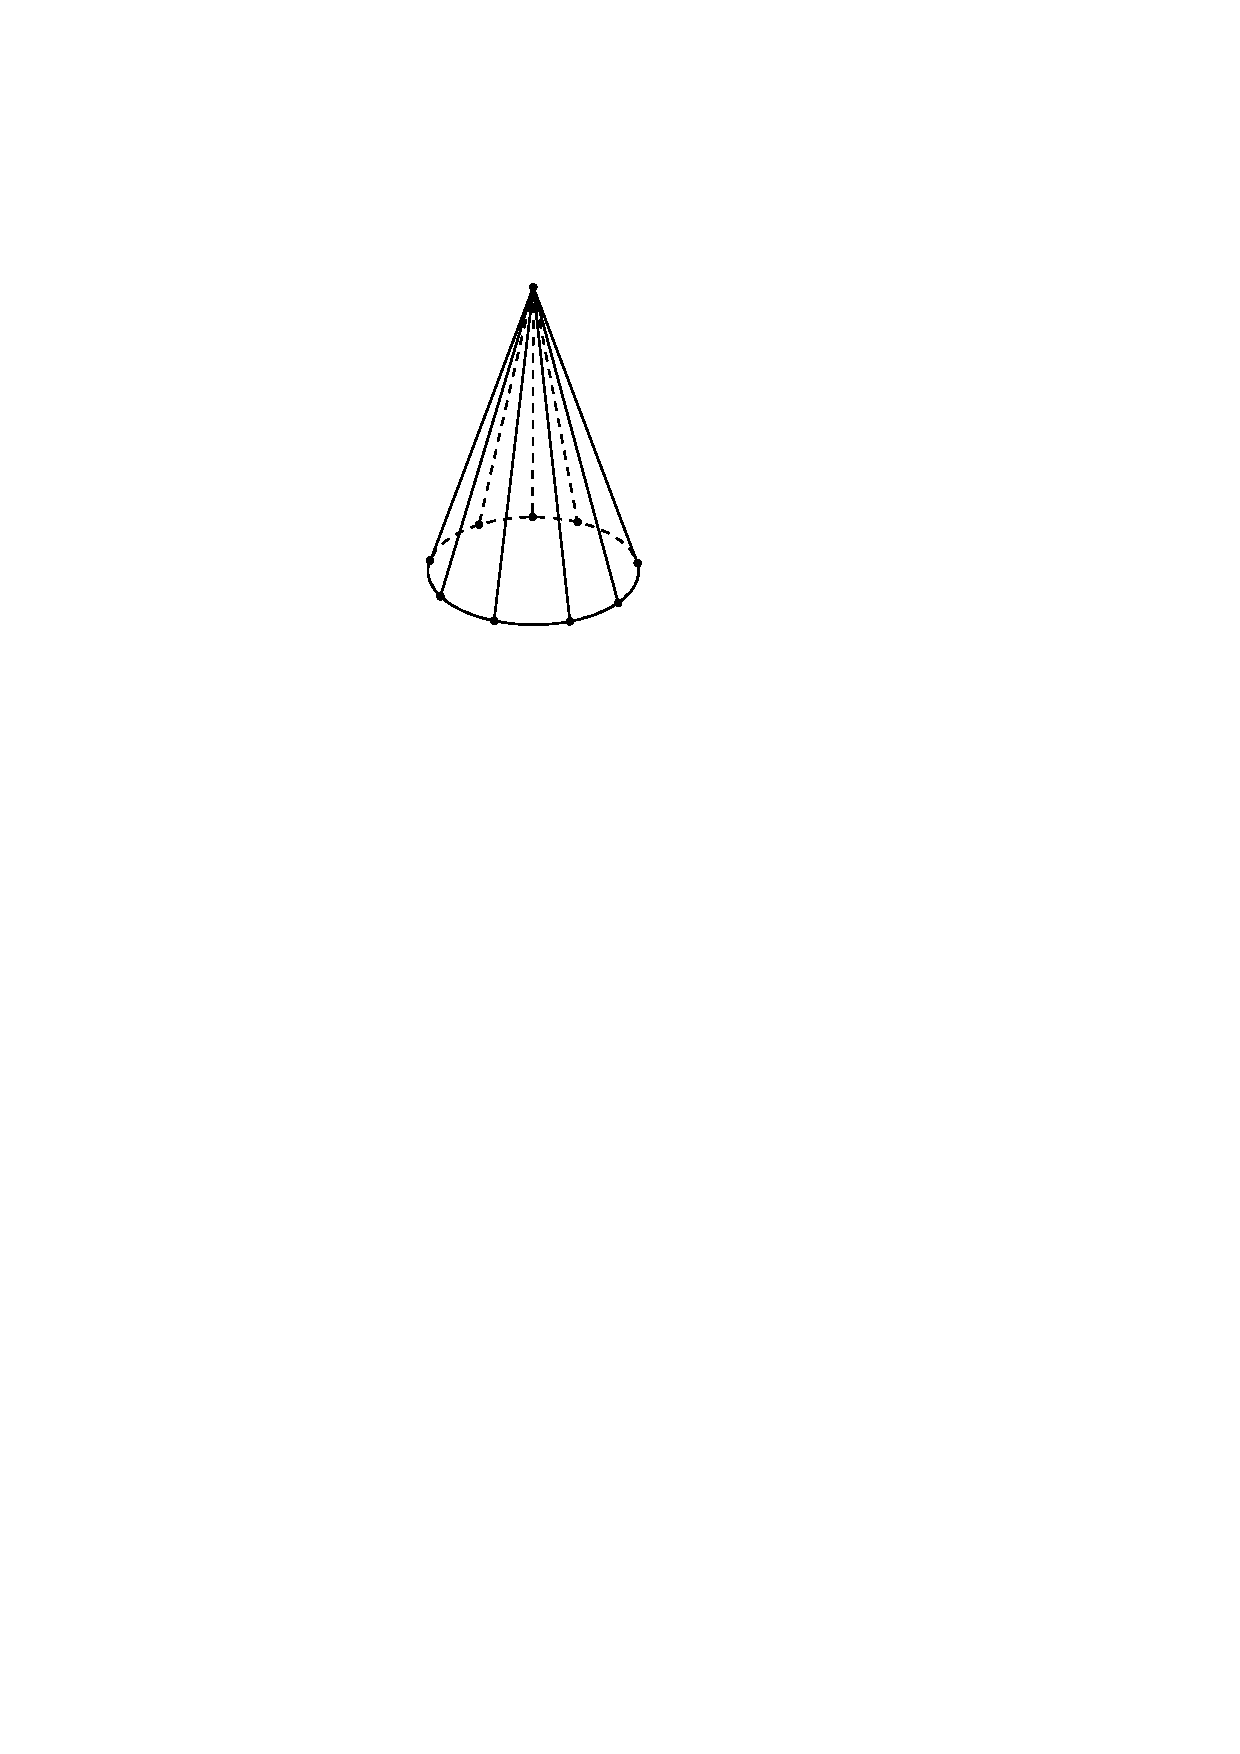
\includegraphics[width=.15\linewidth]{figs/diamond}\hspace{2cm}
    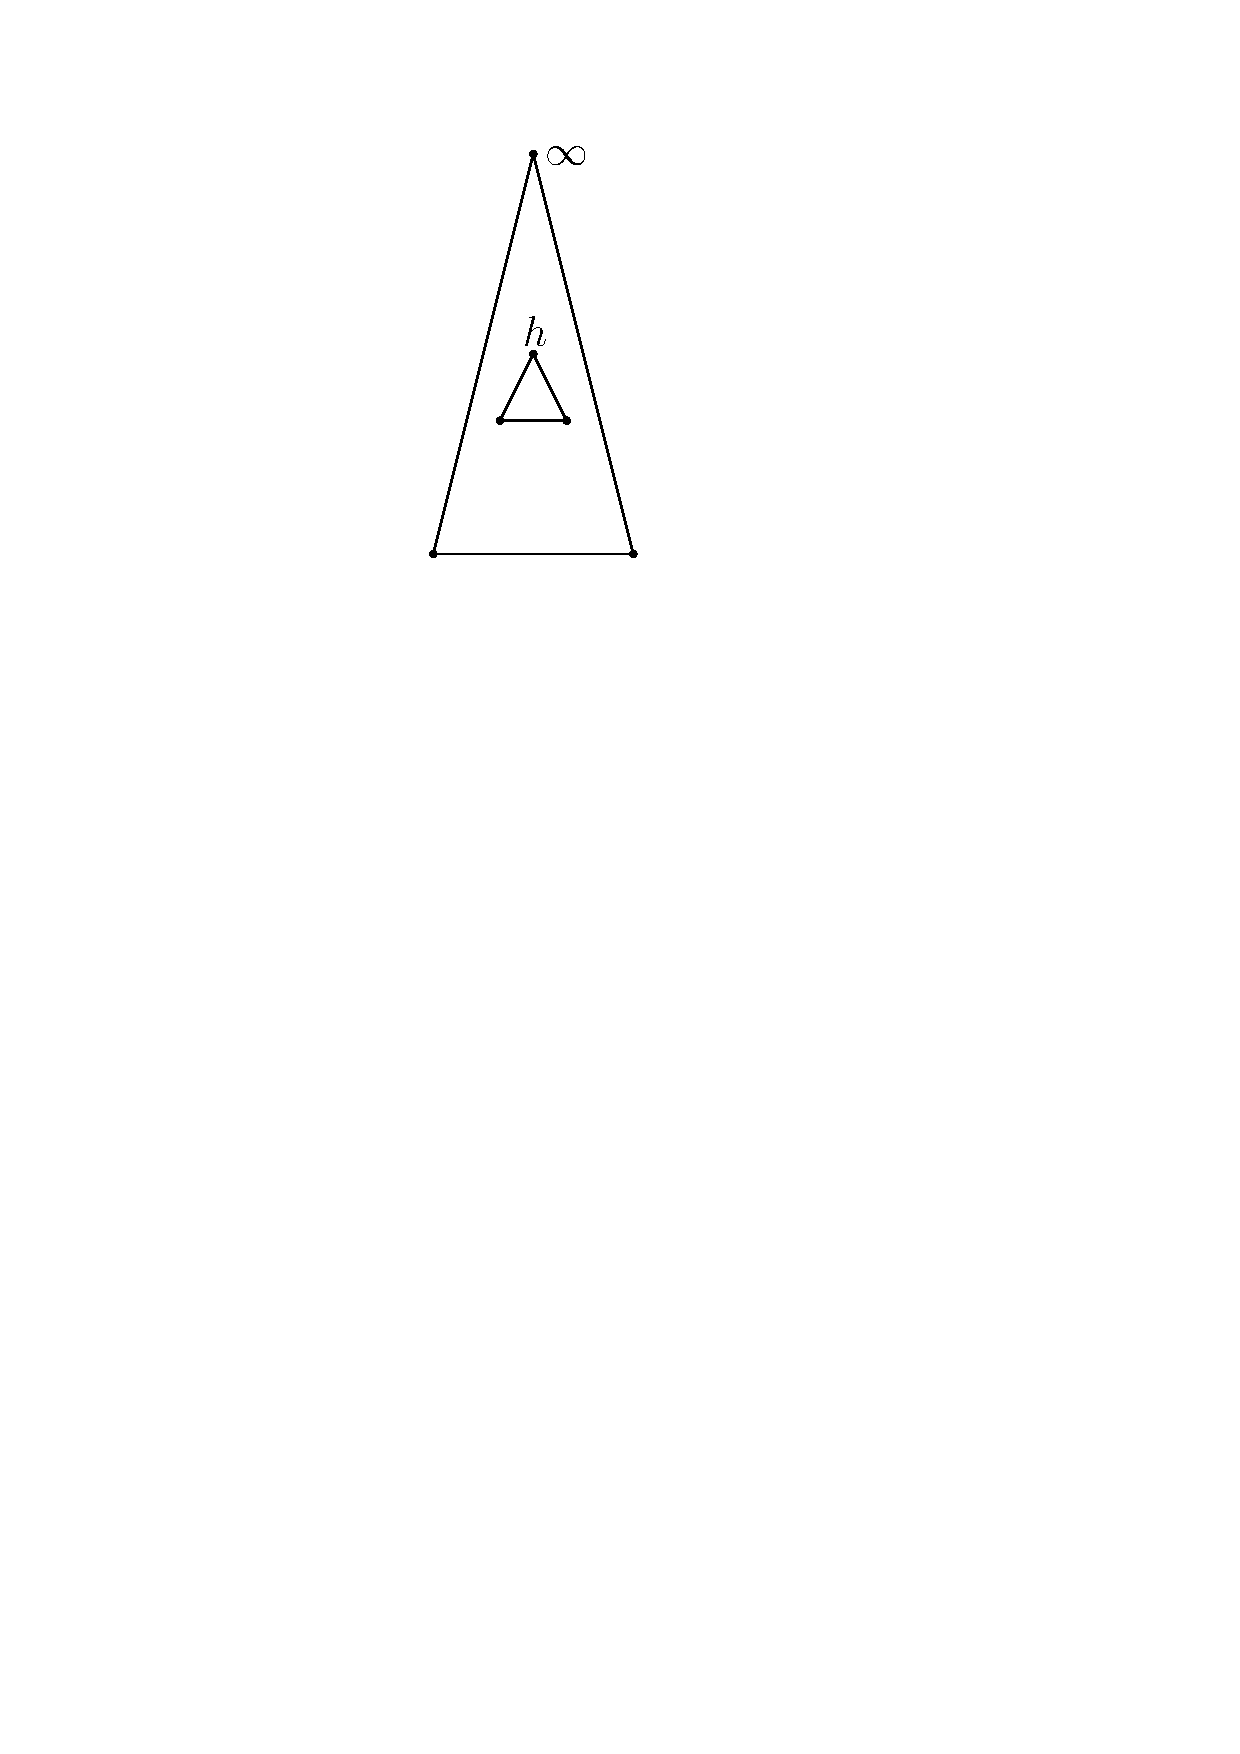
\includegraphics[width=.125\linewidth]{figs/topView}\hspace{2cm}
    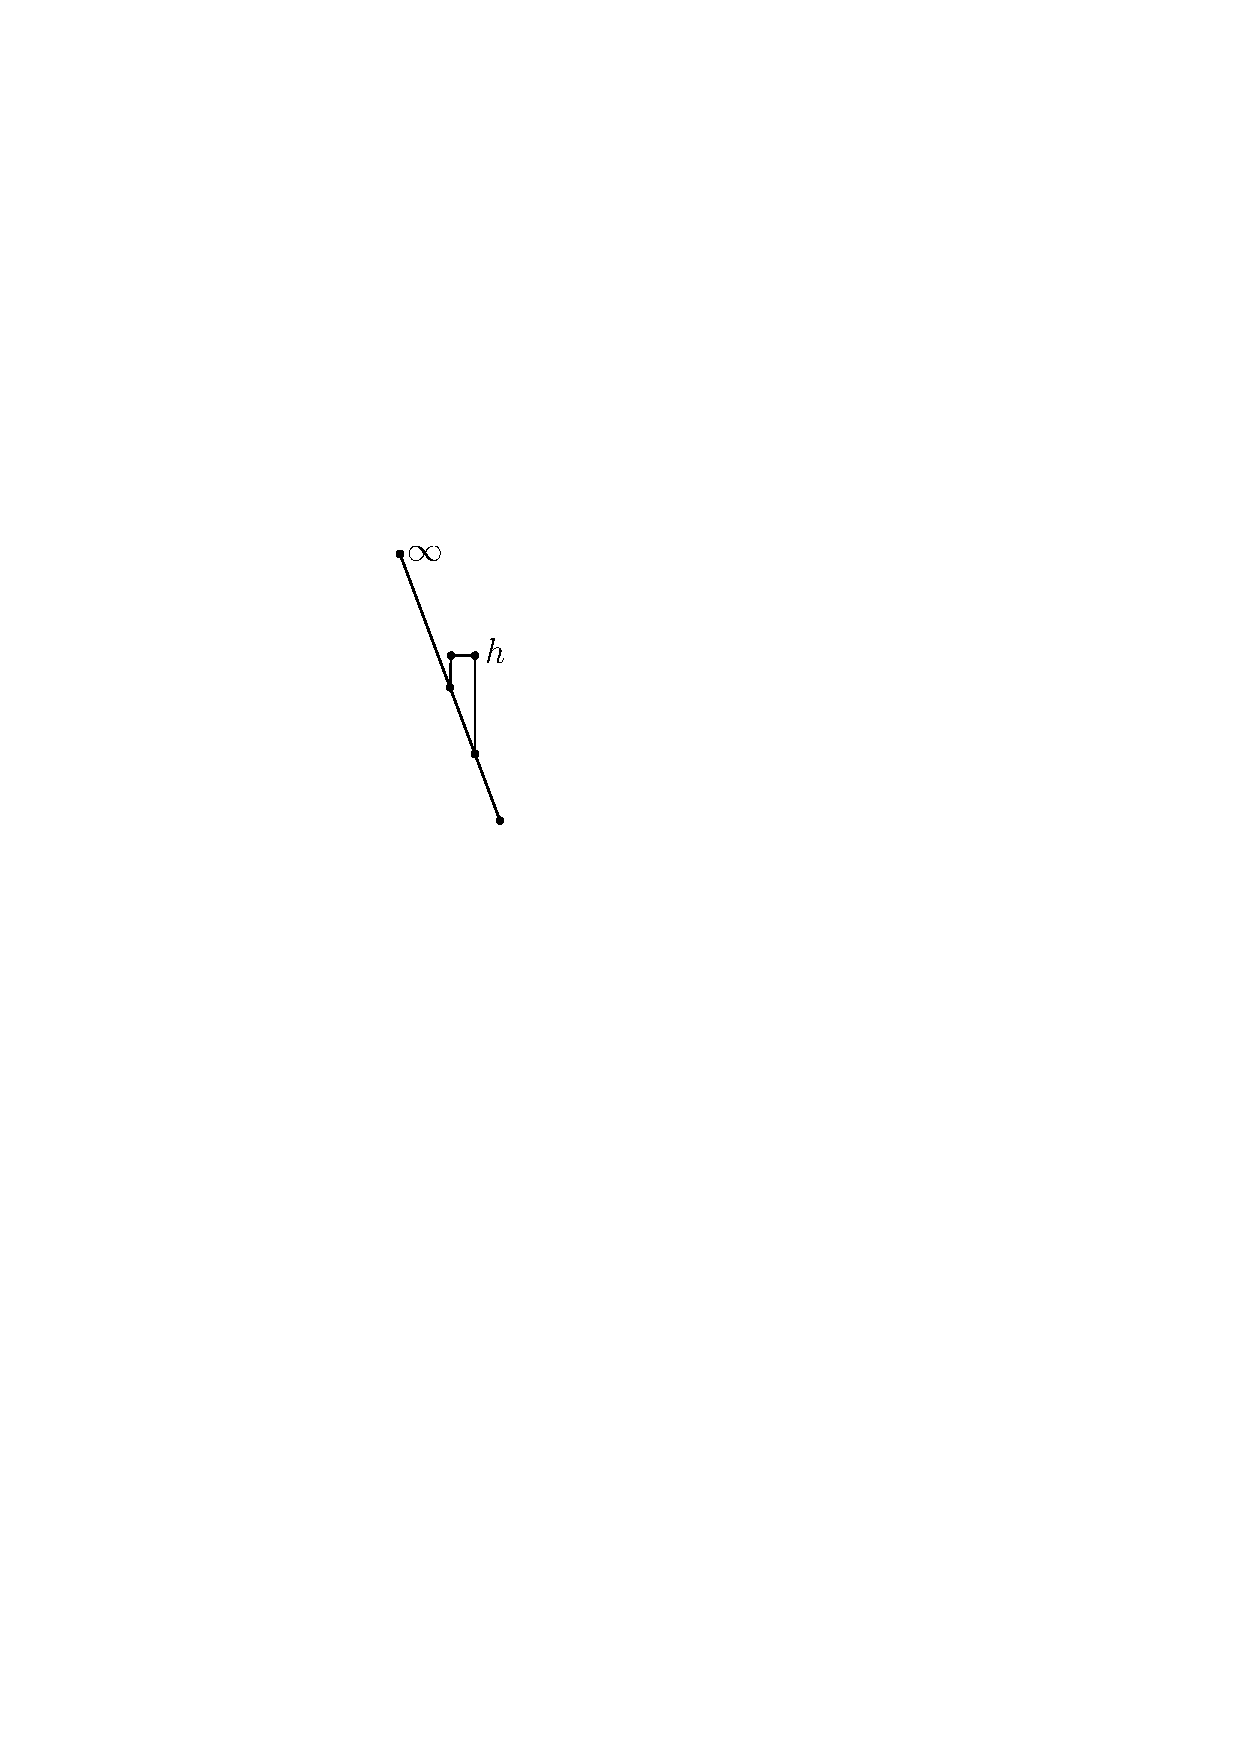
\includegraphics[width=.095\linewidth]{figs/sideView}
    \caption{From left to right: the cone portion of a diamond; the top down view and then the side view of a cone face with a platform added.}
    \label{fig:diamond}
\end{figure}

\begin{lemma}
\label{lem:pathDecomp}
Let $T$ be a merge tree, and let $P = P(T)$ any path decomposition of $T$.  %, and $\pathTree$ the corresponding shrub.  
Then there is a set of at least $\Pi_{p_i\in P} (|p_i|-1)!$ distinct PL $2$-manifolds, all of which have the same defining mesh.
\end{lemma}
\begin{proof}
 We describe a simple mesh, with heights specified for all vertices except for the saddles.  The main idea is that 
 this mesh will be flexible enough to allow almost any assignment of heights to the saddles, thus defining a class of merge trees 
 whose size is that described in the lemma statement.
 
 First, we describe the basic building block of this input mesh, which roughly speaking corresponds to a fixed path $p\in P$.  
 Specifically, we say a \emph{diamond} of size $m$ is the following mesh.  To start, construct a cycle 
 of length $m$, where the height of the $i$th vertex in the cycle is say $i/2m$.  Next, create an apex vertex at height 
 $\infty$ (or any appropriately large finite height), and add an edge between this vertex and each vertex in the cycle.  At this point 
 we have built an upside down cone with $m$ triangular faces (see \Fig{diamond}). To make this cone a closed surface we add a triangular cap at the bottom. 
 Specifically, add a $3$ cycle of vertices at heights $0$, $1/20m$, and $1/10m$, and connect each vertex of this $3$-cycle to an arbitrary distinct 
 vertex on the $m$ cycle (with matching cyclic ordering), and triangulate all remaining faces.  For consistency, if the size $m$ is $\leq 3$, the diamond 
 will be just a tetrahedron.
 
 Now above each face of the cone of the diamond, we will create a triangular ``platform'', which will act as the location to glue on other (shrunken) diamonds, 
 and whose highest point of connection to the face below will be a saddle vertex.  Specifically the heights of the vertices of the triangle will be $h$, $h-\eps$, and $h-2\eps$, where 
 $h$ is some unspecified height value.  This near horizontal platform is then connected to its respective face with vertical edges down to the face. See \Fig{diamond}.
 %
 %The vertex at height $h$ will lie in the plane of the respective face of the cone, and the other two will lie above the face, 
 %with edges connecting down to the face, hence creating an actual ``platform''.
 
 At this point we can construct the entire input mesh, by gluing together diamonds.  
 Specifically, for each path $p_i\in P$ we create a diamond of size $|p_i|-1$ (we subtract one because the tip of the diamond already corresponds to the leaf of the path).
 Now we glue together diamonds of different paths in the same way the paths are connected in the shrub $\pathTree$.  Specially, for two paths $p,q\in P$ where 
 $p$ is the parent of $q$ in $\pathTree$, we glue the bottom triangular cap of the diamond for $q$ onto the triangular ``platform'' of some face of the diamond for $p$.
 (Naturally for this construction to work, diamonds for a given path will be scaled down relative to the size of the diamond of their parent).
 
 Observe now that the only saddle points in this construction are the highest connecting point on a face of an edge from the platform above.  Moreover, the only maxima are the apexes of the 
 diamonds, and there is exactly one minima corresponding to the bottom cap of the diamond representing the root of $\pathTree$.  Therefore, the saddles on a given 
 diamond will appear contiguously on a root to leaf path in the merge tree of the mesh, where the leaf corresponds to the maxima of the diamond 
 (since all these saddles have a direct line of sight to this apex).  In particular, 
 this implies that, regardless of the heights assigned to the platforms, the merge tree of this mesh has a path decomposition whose corresponding shrub is equivalent to $\pathTree$.  
 
 Now there is a valid instantiation of this described mesh for any relative ordering of the heights of the saddles on a given diamond.  In particular, 
 there are $(|p|-1)!$ possible orderings of the heights of the saddles on the diamond for $p$, and hence $\Pi_{p_i\in P} (|p_i|-1)!$ possible instantiations of 
 the mesh overall.  Also, each one of these instantiations will result in a different merge tree.  Specifically, a permutation of the heights on a given diamond 
 corresponds to a permutation of the vertices along a path in $P$, as by construction all saddles on a given diamond will appear in sorted order in the merge tree.
\end{proof}



\begin{corollary}
 \label{cor:mergeLB}
 Let $A(S)$ be any comparison based algorithm to compute the merge tree of any input surface $S$ (whose contour tree is a merge tree).  
 Then the running time of $A(S)$ is $\Omega(f_{path}(P))=\Omega(\sum_{p_i\in P} |p_i|\log|p_i|)$ where $P$ is any path decomposition of the 
 merge tree of $S$.
\end{corollary}
\begin{proof}
 Given an input surface $S$, by the above lemma, any path decomposition $P$ of its merge tree defines a set of $\Pi_{p_i\in P} |p_i|!$ surfaces 
 with distinct merge trees, all of which have the same mesh.  Specifically, for each sorted ordering of the relative height values of the saddles 
 on each diamond in the mesh, yields a different merge tree.
 Therefore, any comparison based algorithm which computes the merge tree must distinguish between these possibilities, and therefore its corresponding decision tree must 
 have $\Pi_{p_i\in P} |p_i|!$ leaves.  Hence by Stirling's approximation, this decision tree must have depth $\Omega(\sum_{p_i\in P} |p_i|\log|p_i|)$.
\end{proof}

\subsection{Contour Trees}
We first generalize previous terms to the case of contour trees.
In this section $T$ will denote an arbitrary contour tree.  Specifically, every internal vertex in $T$ has degree $3$ 
and the height function defined over the vertex set is such that every internal vertex in either a split or merge 
(i.e. at most $2$ neighbors lie above or below it).

Again we define a path decomposition as a partition of the vertices into 
disjoint leaf paths (i.e. each path is monotonic in height and contains a leaf). 
However, for simplicity we now restrict our attention to path decompositions which 
roughly speaking are consistent with the raining procedure described in \Sec{rain} 
(more general decompositions can work, but it is not needed for our purposes).

\begin{definition}
\label{def:path2} A path decomposition, $P(T)$, is called \emph{rain consistent} if its paths can be obtained as follows.
Perform an upward BFS from an arbitrary minima $v$ in $T$, and mark all vertices encountered.  
Now recursively run a directional BFS from all vertices adjacent to the current marked set.  
Specifically, for each BFS run, make it an upward BFS if it is at an odd height in the recursion tree and downward otherwise.  

This procedure partitions the vertex set into disjoint rooted subtrees of $T$, based on which BFS marked a vertex.  
For each such subtree, now take any partition of the vertices into leaf paths.\footnote{Note that the subtree  
of the initial vertex is rooted at is a minima.  For simplicity we require that the path this vertex belongs to 
also contains a maxima.}
\end{definition}


The following is analogous to \Lem{pathDecomp}, and in particular uses it as a subroutine.

\begin{lemma}
\label{lem:pathDecomp2}
Let $T$ be a contour tree, and let $P = P(T)$ be any rain consistent path decomposition of $T$.  
Then there is a set of at least $\Pi_{p_i\in P} (|p_i|-1)!$ distinct PL $2$-manifolds, all of which have the same defining mesh.
\end{lemma}
\begin{proof}
 As $P$ is rain consistent, the paths can be partitioned into sets $P_1, \dots, P_m$, where $P_i$ is the set of all paths with 
 vertices from a given BFS, as described in \Def{path2}.  Specifically, let $T_i$ be the subtree of $T$ corresponding to $P_i$ and 
 let $r_i$ be the root vertex of this subtree.  
 Note that the $P_i$ sets naturally define a tree where $P_i$ is the parent of $P_j$ if $r_i$ is adjacent to a vertex in $P_j$.  
 
 As the set $P_i$ is a path decomposition of a rooted binary tree $T_i$, the surface mesh construction of \Lem{pathDecomp} for $P_i$ is well defined.  
 Actually the only difference is that here the rooted tree is not a full binary tree, and so some of the faces of the constructed diamonds will be blank.  
 Specifically, these blank faces correspond to the adjacent children of $P_i$, and they tell us how to connect the meshes of the different $P_i$'s.
 
\begin{figure}[h]\centering
    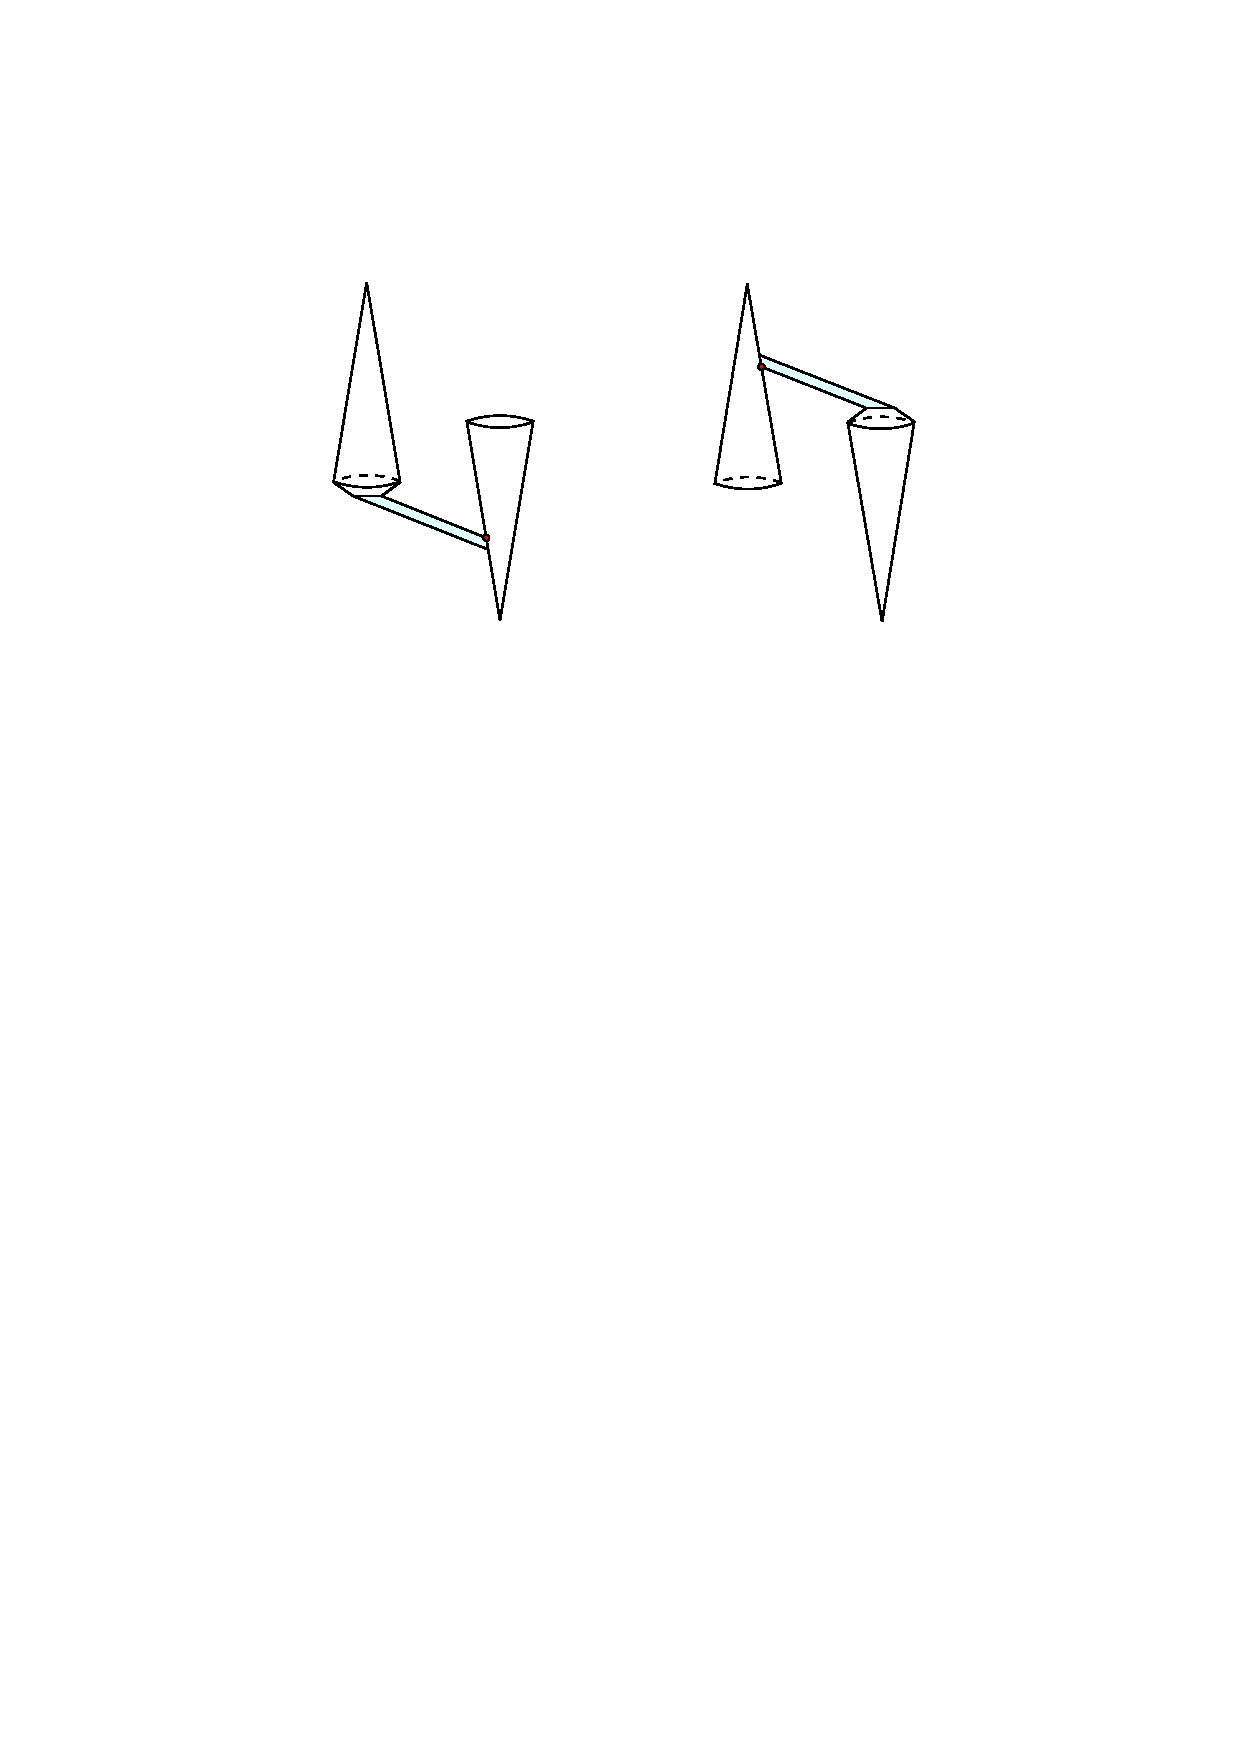
\includegraphics[width=.5\linewidth]{figs/bridge2}
    \caption{On the left, the root of $P_i$ merges into a diamond of its parent $P_j$.  On the right, the root of $P_i$ splits off from a diamond of $P_j$}
    \label{fig:diamond}
\end{figure}
 
 So for each $P_i$ construct a surface mesh as described in \Def{path2}.  By construction, the diamonds corresponding to the paths in $P_i$ are connected 
 into a tree structure (i.e. corresponding to the shrub of $P_i$).  Therefore the bottoms of all these diamonds are covered except for the one corresponding 
 to the path containing the root $r_i$.  If $r_i$ is the initial minima that the rain consistent path decomposition was defined from,  
 we add a tetrahedral cap to the uncovered bottom of this diamond (i.e. we construct the minima).  Otherwise, $P_i$ has some parent $P_j$ in which case 
 we connect the bottom of the diamond for $r_i$ to a free face of a diamond in the construction for $P_j$, specifically, the face corresponding to the 
 vertex in $T$ which $r_i$ is adjacent to. 
 If $T_i$ was created by an upward BFS, then the connection to this face should be a merge vertex, and otherwise it should be a split vertex.  
 See \Fig{diamond}.
 
 Just as in \Lem{pathDecomp} we now have one fixed mesh graph structure, such that each different relative ordering of the heights of the merge and split vertices 
 on each diamond produces a surface with a distinct merge tree.  The specific bound on the number of such distinct manifolds follows by applying the 
 bound from \Lem{pathDecomp} to each $P_i$.
\end{proof}

For the same reason that \Cor{mergeLB} followed from \Lem{pathDecomp}, we now have the following. 

\begin{theorem}
 Let $A(S)$ be any comparison based algorithm to compute the contour tree of an input surface $S$.  
 Then the running time of $A(S)$ is $\Omega(f_{path}(P))=\Omega(\sum_{p_i\in P} |p_i|\log|p_i|)$ where $P$ 
 is any rain consistent path decomposition of the contour tree of $S$.
\end{theorem}




% \section{Temp}
% Given a contour tree we allow any path decomp, as long as each path contains a maxima or minima (or both).
% We call a path $p$ in the decomp a min (resp. max) path if it contains a minima (resp. maxima) (note a path can be both).
% For every path we create a cylinder with $m$ faces for $p$, where $m$ is the number of non-leaf vertices in $p$ (either $|p|-1$ or $|p|-2$).  
% If $p$ has a maxima we put a top cone cap on the cylinder, and if it contains a manima then put a bottom cone cap (i.e. the cap represents the maxima or minima).
% 
% Every edge $e$ in $T$, but not in a path decomp. tells us how to glue together cylinders.  Let $u$ be the upper endpoint of $e$ and $l$ the lower endpoint.
% 
% First we ``remove'' all edges $e$ such that $u$ is adjacent to a max path and $l$ adjacent to a min path by joining the free ends of the respective cylinder together.
% Hence we can assume no such edges exist.  Now we have three cases:
% 
% \begin{enumerate}[{Case} 1]
%  \item 
% $l$ is adjacent to a min path:\newline
% Note in this case the path containing $u$ must be a min path.
% In this case connect the bottom of the cylinder for the path containing $l$ into a face of the cylinder for the path containing $u$.
% \item
% $l$ is adjacent to a max path and $u$ is adjacent to a max path:\newline
% In this case connect the bottom of the cylinder for the path containing $u$ into a face of the cylinder for the path containing $l$.
% \item
% $l$ is adjacent to a max path and $u$ is adjacent to a min path:\newline
% Connect a face of the cylinder for the $u$ path (using a split) to a face of the cylinder for the $l$ path (using a merge).
% \end{enumerate}



\bibliographystyle{alpha}
\bibliography{contour}





%%%%%%%%%%%%%%%%%%%%%%%%%%%%%%%%%%%%%%%%%%%%%%%%%%%%%%%%%%%%%%%%%%%%%%%%%
%%%%%%%%%%%%%%%%%%%%%%%%%%%%%%%%%%%%%%%%%%%%%%%%%%%%%%%%%%%%%%%%%%%%%%%%%
%%%%%%%%%%%%%%%%%%%%%%%%%%%%%%%%%%%%%%%%%%%%%%%%%%%%%%%%%%%%%%%%%%%%%%%%%
%%%%%%%%%%%%%%%%%%%%%%%%%%%%%%%%%%%%%%%%%%%%%%%%%%%%%%%%%%%%%%%%%%%%%%%%%
%%%%%%%%%%%%%%%%%%%%%%%%%%%%%%%%%%%%%%%%%%%%%%%%%%%%%%%%%%%%%%%%%%%%%%%%%
%%%%%%%%%%%%%%%%%%%%%%%%%%%%%%%%%%%%%%%%%%%%%%%%%%%%%%%%%%%%%%%%%%%%%%%%%
%
%
%end of writup
%stuff below should be deleted
%
%
%%%%%%%%%%%%%%%%%%%%%%%%%%%%%%%%%%%%%%%%%%%%%%%%%%%%%%%%%%%%%%%%%%%%%%%%%
%%%%%%%%%%%%%%%%%%%%%%%%%%%%%%%%%%%%%%%%%%%%%%%%%%%%%%%%%%%%%%%%%%%%%%%%%
%%%%%%%%%%%%%%%%%%%%%%%%%%%%%%%%%%%%%%%%%%%%%%%%%%%%%%%%%%%%%%%%%%%%%%%%%
%%%%%%%%%%%%%%%%%%%%%%%%%%%%%%%%%%%%%%%%%%%%%%%%%%%%%%%%%%%%%%%%%%%%%%%%%
%%%%%%%%%%%%%%%%%%%%%%%%%%%%%%%%%%%%%%%%%%%%%%%%%%%%%%%%%%%%%%%%%%%%%%%%%
%%%%%%%%%%%%%%%%%%%%%%%%%%%%%%%%%%%%%%%%%%%%%%%%%%%%%%%%%%%%%%%%%%%%%%%%%






\remove{

\appendix

\section{Old stuff}

\subsubsection{Paying it down the line}

% \begin{claim}
% \label{clm:sizes}
%  Let $p$ be a path in a maximum path decomposition, such that $|H_p|>c|p|$ for some constant $c> 6$.
%  Let $H_f$ denote the heap at the leaf of $p$.  We then have the following
%  \begin{compactenum}
%   \item $|H_f|\leq (1+1/c)|H_p|$
%   \item $|H_f|\geq |H_p|/3$
%   \item For any path $q$ adjacent to $p$ in the shrub, $|H_q|<\frac{2}{3}|H_p|$
%  \end{compactenum} 
% \end{claim}
% \begin{proof}
%   For any vertex $v\in p$ \Obs{decrease} implies that $|H_v|\leq |H_p| + |p| < (1+1/c) |H_p|$.
%   First observe that by setting $v=f$ this immediately implies the first part of the claim.
%  % By a similar argument, $|H_f|\geq |H_p| - |p| > (1-1/c)|H_p|$.
%   
%   To prove the last part of the claim, suppose otherwise that $|H_q|\geq \frac{2}{3}|H_p|$ for some 
%   adjacent path $q$.  As this is a maximum path decomposition, this implies that there is some 
%   $v\in p$ such that $|H_v|\geq \frac{4}{3}|H_p|-1$.
%   By \Obs{decrease} we then have, 
%    $|H_p| \geq |H_v| - |p|\geq \frac{4}{3}|H_p| - 1 - |H_p|/c \geq (4/3-1/c)|H_p|-1$.
%   When rearranged this gives $1\geq (1/3-1/c)|H_p|$.  As $c>6$ we have $1\geq |H_p|/6$, 
%   which is a contradiction as $|H_p|>c|p|>6$.
% \end{proof}

\Ben{I had originally thought the following claim would be useful in proving the lemma below.}
\begin{claim}
\label{clm:sizes}
 Let $p$ be a path in a maximum path decomposition, such that $|H_p|>c|p|$ for some constant $c> 6$.
 We then have the following
% \begin{compactenum}
%  \item 
  For any path $q$ adjacent to $p$ in the shrub, $|H_q|<\frac{2}{3}|H_p|$
%  \item If there does not exist and adjacent path $q$ such $H_q\geq H_p/3$, then $|H_f|\geq |H_p|/3$
% \end{compactenum} 
\end{claim}
\begin{proof}
  To prove the claim, suppose otherwise that $|H_q|\geq \frac{2}{3}|H_p|$ for some 
  adjacent path $q$.  As this is a maximum path decomposition, this implies that there is some 
  $v\in p$ such that $|H_v|\geq \frac{4}{3}|H_p|-1$.
  By \Obs{decrease} we then have, 
   $|H_p| \geq |H_v| - |p|\geq \frac{4}{3}|H_p| - 1 - |H_p|/c \geq (4/3-1/c)|H_p|-1$.
  When rearranged this gives $1\geq (1/3-1/c)|H_p|$.  As $c>6$ we have $1\geq |H_p|/6$, 
  which is a contradiction as $|H_p|>c|p|>6$.  
\end{proof}

\begin{lemma}
\label{lem:excess}
 Let $p$ be a tall path, and let $S_1, \dots S_k$ and $R_1, \dots, R_l$ be the sizes of the heaps at the roots of the short and tall children of $p$, respectively, in the shrub.  
 Let $H_f$ be the heap at the leaf of the path $p$.
 Then,  $|H_p| \log |H_p|   \geq  \sum_{v\in p} \log|H_v| + \frac{4}{3}\sum_{i=1}^k S_i \log S_i + \sum_{i=1}^l R_i \log R_i  -  c|p|\log |p|$, for some sufficiently large constant $c$
 \end{lemma}
\begin{proof}
 First observe that the lemma holds for $|H_p|$ less than any fixed constant, since otherwise \Lem{adjacent} implies we can choose $c$ 
 large enough such that $c|p|\log|p|$ will dominate all other terms.
 Next, observe that $\sum_{v\in p} \log|H_v| \leq \sum_{v\in p} \log(|H_v|+|p|) = |p|\log(|H_v|+|p|) = O(|p|\log|p|)$, as $p$ is a tall path.  
 Therefore, in the remainder of the proof  we can safely ignore the $\sum_{v\in p} \log|H_v|$ term as we can choose $c$ large enough to cover it.  
 That is we now instead prove the inequality,
 \[
  |H_p| \log |H_p|   \geq \frac{4}{3}\sum_{i=1}^k S_i \log S_i + \sum_{i=1}^l R_i \log R_i  -  c|p|\log |p|
 \]
 To do so we  break the analysis into two case based on the relative size of $|p|$ and $|H_p|$. 
 In the following, $\alpha>10$ is some yet to be determined constant.  

\paragraph{Case 1, $|p|\geq |H_p|/\alpha$:\\}
First observe that by \Lem{adjacent}, $|H_p|+|p| \geq \sum_{i=1}^k S_i+ \sum_{i=1}^l R_i$.
By choosing $c$ large enough we therefore have,
\begin{align*}
 c|p|\log|p| &\geq 2(1+\alpha)^2 |p|\log |p| \geq 2(1+\alpha)|p| \log((1+\alpha)|p|)\\
             &\geq 2(|H_p|+|p|)\log(|H_p|+|p|) \geq 2\log(|H_p|+|p|) \pth{\sum_{i=1}^k S_i + \sum_{i=1}^l R_i}\\
             &\geq \frac{4}{3}\sum_{i=1}^k S_i \log S_i + \sum_{i=1}^l R_i \log R_i 
\end{align*}



In this case $\log(|H_p|+|p|)\leq \log(2|p|) \leq 1+\log(|p|)$ (where $\log$ is base $2$).
Therefore, assuming $|p|>1$, we have 
\[
(|H_p|+|p|)\log(|H_p|+|p|)\leq (1+c)|p|\log((1+c)|p|) %(|H_p|+|p|)(1+\log |p|) \leq 2(1+c)|p|\log |p|
\]
which when combined with the inequality from \Lem{adjacent} gives, 
\[
 4(1+c)|p|\log |p| \geq 2(|H_p|+|p|)\log(|H_p|+|p|)\geq \pth{|H_f| + \frac{4}{3}\sum_{i=1}^k S_i + \sum_{i=1}^l R_i}\log(|H_p|+|p|).
\]
This easily implies the desired inequality as $\log(H_p+p)$ is larger than any other $\log$ term in the inequality.

\paragraph{Case 2, $|p|< |H_p|/\alpha$:\\}

\Ben{Was not able to handle this case.}

%  First, lets assume we can show $\sum_{i=1}^k S_i + \sum_{i=1}^l R_i \leq \frac{3}{4}|H_p|$.  
%  In this case, using the last part of \Clm{sizes}, we can prove the desired inequality as follows.
%  
%  \begin{align*}
%   \frac{4}{3}\sum_{i=1}^k S_i \log S_i + \sum_{i=1}^l R_i \log R_i  &\leq  \frac{4}{3} \pth{\sum_{i=1}^k S_i \log S_i + \sum_{i=1}^l R_i \log R_i} \\
%   &\leq  \frac{4}{3} \log |H_p| \pth{\sum_{i=1}^k S_i + \sum_{i=1}^l R_i}  \leq  |H_p| \log |H_p|
%  \end{align*}
%  
%  Finally, to complete the proof we must prove our assumption that $\sum_{i=1}^k S_i + \sum_{i=1}^l R_i \leq \frac{3}{4}|H_p|$.
%  By \Lem{adjacent} and \Clm{sizes} we have, 
%  \[
%  \sum_{i=1}^k S_i + \sum_{i=1}^l R_i 
%  \leq |H_p|+|p|-|H_f| 
%  \leq (1+1/\alpha-1/3)|H_p| = (2/3+1/\alpha)|H_p|
%  \]
%  
%  Therefore $\sum_{i=1}^k S_i + \sum_{i=1}^l R_i \leq \frac{3}{4}|H_p|$ if $(2/3 + 1/\alpha)\leq 3/4$, which rearranged gives $\alpha \geq 12$
\end{proof}





\remove{
% \subsubsection{Paying it down the line}
% 
% \begin{lemma}
% \label{lem:excess}
%  Let $p$ be a tall path, and let $S_1, \dots S_k$ and $R_1, \dots, R_l$ be the sizes of the heaps at the roots of the short and tall children of $p$, respectively, in the shrub.  
%  Let $H_f$ be the size of the heap at the leaf of the path $p$, and let $X = \sum_{i=0}^k H_i \log H_i$.  
%  Then,  $|H_p| \log |H_p|   \geq  H_f\log H_f + \sum_{i=0}^k S_i \log S_i + \sum_{i=0}^l R_i \log R_i  -  c|p|\log |p|$, for some sufficiently large constant $c$
%  \end{lemma}
% \begin{proof}
% By \Lem{adjacent} we know that $|H_p|+|p| \geq  H_f + \sum_{i=0}^k S_i + \sum_{i=0}^l R_i$.  
% %Now as $p$ is a tall path we have $|p|\geq \sqrt{|H_p|}/100$, and so, $(|H_p|+|p|)\log(|H_p|+|p|)$
% 
% We  break the analysis into two case based on the relative size of $|p|$ and $|H_p|$.  In the following $c$ is some yet to be determined constant greater than $1$.
% 
% \paragraph{Case 1, $|p|\geq |H_p|/c$:}  
% In this case $\log(|H_p|+|p|)\leq \log(2|p|) \leq 1+\log(|p|)$ (where $\log$ is base $2$).
% Therefore, assuming $|p|>1$, we have 
% \[
% (|H_p|+|p|)\log(H_p+p)\leq (|H_p|+|p|)(1+\log |p|) \leq (2|p|)(2\log |p|)\leq 4|p|\log |p|
% \]
% which when combined with the inequality from \Lem{adjacent} gives, 
% \[
%  4|p|\log |p| \geq (|H_p|+|p|)\log(|H_p|+|p|)\geq \pth{H_f + \sum_{i=0}^k S_i + \sum_{i=0}^l R_i}\log(|H_p|+|p|).
% \]
% This easily implies the claim as $\log(H_p+p)$ is larger than any other $\log$ term in the inequality.
% 
% \paragraph{Case 2, $|p|< |H_p|/c$:}
% \end{proof}
}


Define the crust of the shrub to be the first (i.e. closest to the root) layer of short paths in the shrub.  Apply \Lem{shortCost} to each of the short paths in the crust and then 
say by \Lem{excess} and since the root heap goes to zero we are done.



\ignore{
Naturally, this geometric series behavior can be extended to more than two adjacent short paths, thus motivating 
the following definition.

\begin{definition}
 Let $p$ be a path in a path decomposition $P(T)$, with corresponding shrub $\pathTree$.
 Call a short path $q\in P(T)$ short reachable from $p$ if the path from $p$ to $q$ in $\pathTree$ 
 contains only vertices which correspond to short paths.  Call the subtree of $\pathTree$ consisting 
 of all short reachable paths from $p$ the \emph{short shrub} of $p$, and denote it $\mathcal{L}(p)$.
\end{definition}

In the following subsection we show how to exploit this geometric series behavior of short shrubs.

We say two paths in $P(T)$ are adjacent if their corresponding vertices are adjacent in the shrub.  Similarly, for 
two adjacent paths in $P(T)$ we can define a parent/child relationship based on this relationship in the shrub. 
}

\remove{
\Ben{Maybe move the remainder of this subsection to 5.3 since tall and short paths and not used until then}

\begin{definition}
 Let T be a binary tree and let $\chi(T)$ and $P(T)$ be a valid coloring and path decomposition of $T$, respectively.  
 For $p\in P(T)$, we say that $p$ is \emph{short} if $|p| < \sqrt{|H_{r_p}|}/100$, and we say it is \emph{tall} otherwise.
\end{definition}

\begin{observation}
\label{obs:decrease}
 Let $v$ be a vertex in $T$ and let $w$ be its parent.  Then $|H_w| \geq |H_v| -1$, as $L(T_v) \subseteq L(T_w)$ and the path from 
 $w$ to the root has one less vertex than the path from $v$ to the root.
 
 In particular, we have the following more general property.
 Let $v$ and $u$ be any two vertices in the same root to leaf path of $T$, such that $u$ is lower than $v$.  
 Then $|H_v| \leq |H_u| + d(u,v)$. 
\end{observation}


\begin{lemma}
\label{lem:pathBounds}
 Let T be a binary tree and let $\chi(T)$ and $P(T)$ be a valid coloring and path decomposition of $T$, respectively.
 Then, 
 \begin{compactenum}
  \item for any tall path $p\in P(T)$, $\sum_{v\in p} \log |H_v| = O(|p| \log |p|)$.
  \item for any short path $p\in P(T)$, $\sum_{v\in p} \log |H_v| = O(|p| \log |H_{r_p}|)$.
 \end{compactenum}
\end{lemma}
\begin{proof}
 By $\Obs{decrease}$ we know that for any vertex $v\in p$, $|H_v|\leq |H_{r_p}| + |p|$ (as $r_p$ lies below $v$ on $p$).
 As such, 
 \[
 \sum_{v\in p} \log |H_v| \leq \sum_{v\in p} \log(|H_{r_p}| + |p|)  = |p| \log (|H_{r_p}| + |p|).
 \]
 If $p$ is a tall path then $|p| \log (|H_{r_p}| + |p|) = O(|p| \log |p|)$, and if $p$ is short then 
 $|p| \log (|H_{r_p}| + |p|) = O(|p| \log |H_{r_p}| )$.
\end{proof}

The following lemma can be thought of as a generalization of $\Obs{decrease}$.

\begin{lemma}
\label{lem:adjacent}
 Let $T$ be a binary tree and let $\chi(T)$ and $P(T)$ be a valid coloring and path decomposition of $T$, respectively.
 Let $p$ be any path in $P(T)$ and let $\{q_1, \dots q_k\}$ be the set of all adjacent child paths of $p$.
 For $1\leq i\leq k$ let $r_i = r_{q_i}$ and let $H_i = H_{r_i}$.
 Also, let $H_0$ denote the heap at the leaf of $p$.
 
 Then $\sum_{i=0}^k |H_i| \leq |H_p|+|p|$, where $H_p = H_{r_p}$.
\end{lemma}
\begin{proof} 
 First observe that for all $i$, $r_{i}$ lies above $r_p$ on some root to leaf path. 
 Let $H_i'$ be the subset of $H_i$ that lies below $r_p$.  Observe that $H_i'\subseteq H_p$, as $L(T_{r_i})\subseteq L(T_{r_p})$.
  
 Now for any $i\neq j$, $H_i \cap H_j = \emptyset$, as $r_{i}$ and $r_{j}$ are not on the same root to leaf path (i.e. $L(T_{r_i}) \cap L(T_{r_j}) = \emptyset$).
 In particular, $(H_i\setminus H_i') \cap (H_j \setminus H_j') = \emptyset$, and so $\sum_{i=0}^k |H_i\setminus H_i'| \leq |p|$ 
 as $H_i\setminus H_i'$ is precisely the subset of $H_i$ that lies on $p$.
 Moreover, for any $i\neq j$, $ H_i' \cap H_j' = \emptyset$, and so since $H_i'\subseteq H_p$ we have $\sum_{i=0}^k |H_i'|\leq |H_p|$.
 Putting these together gives
 \[
  \sum_{i=0}^k |H_i| = \sum_{i=0}^k |H_i'| + \sum_{i=0}^k |H_i\setminus H_i'| \leq |H_p|+|p|.
 \]
\end{proof}

% \Ben{There is a fundamental flaw in the following lemma and corollary.  
% As such, the remainder of this subsection will likely be deleted.}
% 
% Using the notation defined in the above lemma, we have the following crucial lemma, which we will use to 
% argue we can charge that cost of all paths in $P(T)$ to the cost of the tall paths.
% 
% \begin{lemma}
% Let $p$ be a tall path in $P(T)$ and let $\{q_1, \dots q_k\}$ be any set of short paths in $P(T)$ such that 
% $\sum_{i=1}^k |H_i| = O(H_p)$.  Then $\sum_{i=1}^k \sum_{v\in q_i} \log |H_v| = O(|p|\log |p|)$
% \end{lemma}
% \begin{proof}
% By \Lem{pathBounds}, for all $1\leq i\leq k$, 
%  $\sum_{v\in q_i} \log |H_v| = O(|q_i|\log |H_i|) = O(|H_i|\log |H_i|)$, as $q_i$ is a short path.
%  By assumption $\sum_{i=1}^k |H_i| = O(|H_p|)$, 
%  As $x\log x$ is a convex function, Jensen's inequality then implies 
%  $\sum_{i=1}^{k} |H_i|\log |H_i| = O(|H_p| \log |H_p|) = O(|p|\log |p|)$, since $p$ is a tall path.
% \end{proof}
% 
% 
% \begin{corollary}
% \label{cor:tallLight}
%  Let $p$ be a tall path in $P(T)$ and let $\{q_1, \dots q_k\}$ be the set of all short paths adjacent to $p$.
%  Then $\sum_{i=1}^k \sum_{v\in q_i} \log |H_v| = O(|p|\log |p|)$.
% \end{corollary}
% \begin{proof}
%  Let $H_i$ be as defined in \Lem{adjacent}.  By \Lem{pathBounds}, for all $1\leq i\leq k$, 
%  $\sum_{v\in q_i} \log |H_v| = O(|q_i|\log |H_i|) = O(|H_i|\log |H_i|)$, as $q_i$ is a short path.
%  Now by \Lem{adjacent}, $\sum_{i=1}^k |H_i| \leq |H_p|+|p| = O(|p|)$, as $p$ is a tall path. 
%  Therefore, as $x\log x$ is a convex function, Jensen's inequality implies the claim.
%  
% \end{proof}

}



\subsection{The shrub of unsupported paths} \label{sec:short}



It suffices to focus on unsupported short paths. \Lem{short} can be reduced to the following.

\begin{lemma} \label{lem:support} $\sum_{p \in \cL \setminus \cL'} \sum_{v \in p} \log |H_v| = O(\sum_{p \in \cL'} |H_p| \log |H_p|)$.
\end{lemma}

We now construct the shrub of unsupported short paths. Consider $p \in \cL \setminus \cL'$,
and traverse the chain of ancestors from $p$. Eventually, we must reach another short path $q$.
(If not, we have reached the root $r$ of $\pmax(T)$. Hence, $p$ is supported.)
Insert edge from $p$ to $q$, so $q$ is the parent of $p$ in $\cU$. This construction leads
to the shrub forest of $\cL \setminus \cL'$, where every unsupported short path is an internal node, and all
roots are supported short paths. 

We list out some important claims about this shrub forest.
We focus on $\cU$, a connected component (shrub) in the shrub forest and denote the 
the root by $r(\cU)$.

\begin{claim} \label{clm:loss2} Consider $p \in \cL \setminus \cL'$ that is in $\cU$. Let $Q$
be the set of tall ancestors of $p$ that are descendants of $r(\cU)$. Then $\sum_{q \in Q} |q \cap H_p| \leq |H_p|/50$.
\end{claim}

\begin{proof} Suppose not, for contradictions sake. As we traverse the tall ancestors of $p$,
we encounter various vertices of $H_p$ in the ancestors $q$. Consider the first $|H_p|/100$
such vertices of $p$ encountered. At each such $v$, there are at least $|H_p|/100$
vertices \emph{not yet} encountered, so $|H_v| > |H_p|/100$. Each of these vertices $v$
is supported, implying that $p$ is a supported short path.
\end{proof}

\Lem{support} is a direct consequence of the following,
which is the really the main lemma.

%\begin{lemma} \label{lem:cu} Let $\cU$ denote a connected component (shrub) in the shrub forest of $\cL \setminus \cL'$ and let $r$
%be the root of $\cU$. Then $\sum_{p \in \cU} \sum_{v \in p} \log |H_v| = O(|H_r| \log |H_r|)$.
%\end{lemma}
%
%We proceed with the setup to prove \Lem{cu}.
%We focus our attention on some shrub $\cU$.
%We prove a technical lemma about $\cU$, from which \Lem{cu} follows directly.

\section{Ben's old stuff}



\begin{proof} (part (ii) of \Lem{cu-root}) Let level $\ell$ of $\cU$ denote all nodes at distance $\ell$ from the root $r$.
These set of these nodes is designated as $\cU_\ell$. We set $\sigma_\ell = \sum_{p \in \cU_\ell} |p|$
and $\sigma_{\leq \ell} = \sum_{k \leq \ell} \sigma_k$.
By \Lem{geometric}, for any $p \in \cU_\ell$, $|H_p| \leq (2/3)^\ell |H_r|$.

Since all nodes in $\cU$ represent short paths, $\forall p \in \cU$, $|p| < \sqrt{|H_p|}/100$.
So $\sigma_\ell < \sum_{p \in \cU_\ell} \sqrt{|H_p|}/100$. 

\end{proof}


To prove this, we need to understand how $H_p$ is constructed. The path $p$ has some children
$q_1, q_2, \ldots, q_k$ in $\pmax(T)$. Furthermore, as a leaf path in $p$, some leaf
$\ell$ of $T$ in one of the ends of $p$. The heap $H_p$ is essentially the
union of $H_\ell$ and $H_{q_1}, H_{q_2}, \ldots, H_{q_k}$, with the vertices in $p$
removed. Note that some of the $q_i$'s are the corresponding $h(q')$ vertices,
for a child $q'$ in $\cU$.


Let $\mathcal{L} = \mathcal{L}(r)$ be a short shrub of some short path $r$ in a maximum path decomposition $\mathcal{P}(T)$.
The intuitive idea is that due to the geometric decreasing behavior of short shrubs described in the previous subsection, 
one can show that for the entire short shrub our algorithm pays roughly the cost due to the root path $r$.  This argument 
is hard to make directly, so instead we define an alternative quantity for which we can make the argument.
Specifically, we now define a weight function $w(v)$ for all $v\in \mathcal{L}$, and show that $w(v)=\Theta(|H_v|)$.  

For a path $v\in \mathcal{L}$, let $H_v$ denote the heap at the root of $v$, and let $H_{v_f}$ denote the heap 
at the leaf of $v$.  Let $S_l(v)$ (resp. $S_h(v)$) be the subset of short (resp. tall) paths adjacent to $v$ in $\pathTreeA(T)$.

We want to understand how the heap size changes as we move around the paths in $\mathcal{L}$.  Specifically, there are 
three places the vertices in the heap along a short path can come from; adjacent short paths, adjacent tall paths, and the initial heap at the leaf of the path.  
Given this observation we now define a weight function which upper bounds the size of the heap at the root of any path in $\mathcal{L}$.

First, for all $v\in \mathcal{L}$ we define the local cost function $c(v) = H_{v_f}+\sum_{i\in S_h(v)} H_i$, this is the addition to the heap at $v$ which 
was not already charged to descendant short paths.  We now define a weighted version of $\mathcal{L}$ based on these costs.  
To do so, we first augment $\mathcal{L}$ by attaching one 
leaf to each vertex in $\mathcal{L}$.  Now for each newly created leaf (which are the only leaves now) assign the cost 
$c(v)$ defined above, where $v$ is that leaf's corresponding parent.  
Now we can define a weight function $w(u)$ over any node $u$ in the tree, which is defined to be the total cost of all leaves in its subtree.   
To simplify notation, we now use $\mathcal{L}$ to refer to this new weighted tree (rather than its unweighted counterpart).

As the weight $w(p)$ includes the sizes of the heaps of all contributing tall paths and leaves in the subtree rooted at $p$, we have the following.

\begin{claim}
For any $p\in \mathcal{L}$, $w(p)\geq |H_p|$.  Moreover, for any $v\in p$, $w(p)\geq |H_v|$.
\end{claim}

%Let $W= \sum_{v\in \mathcal{L}} w(v) \geq \sum_{v\in \mathcal{L}} |H_v|$.  
%Suppose we could show that conversely $W=O(H_r)$.  Then we would have 
%$\sum_{v\in \mathcal{L}} H_v = O(H_r)$, which was our original goal.  
%So proving $W=O(H_r)$ is now our new goal.

We now would like to show conversely that $w(v)= O(|H_v|)$.  
To do so we first introduce some notation.  
Let $C\subseteq \mathcal{P}$ be the subset of paths that are leaves in $\mathcal{L}$.
For any path $v$, let $\mathcal{L}_v$ (resp. $C_v$) be the subset of paths in $\mathcal{L}$ (resp $C$) 
that are in the subtree of $\mathcal{L}$ which is rooted at $v$.

First, observe that $|H_v|\geq w(v)-\sum_{u\in \mathcal{L}_v} |u|$.  
This holds by the same argument as in \Lem{adjacent}, namely, $w(v)$ by definition 
counts all the contributing tall path heaps and initial leaf heaps that contribute 
to the heap at $v$ and $\sum_{u\in \mathcal{L}_v} |u|$ is an upper bound on the number 
of vertices that could have been removed from one of these heaps before reaching the 
root of $v$ (since a vertex in a heap can only get removed if it appears on one of 
the paths).  

As all paths in $\mathcal{L}$ are short, we thus have the following.

\begin{claim}
$|H_v|\geq w(v)-\sum_{u\in \mathcal{L}_v} \sqrt{|H_u|}/100 \geq w(v)-\sum_{u\in \mathcal{L}_v} \sqrt{w(u)}/100$
\end{claim}

By the above claim, if we can prove $\sum_{u\in \mathcal{L}_v} \sqrt{w(u)}/100 \leq w(v)/c$ for some constant $c>1$, 
then we will have proven that $|H_v| = \Theta(w(v))$.  

Recall that \Lem{geometric} told us that that $|H_{u}|\leq (3/5) |H_{u'}|$, if $u'$ is the parent $u$ in $\mathcal{L}$. 
The following lemma shows that if we had a similar statement in terms of the weights rather than the heap sizes, 
then we get the desired bound on the sum.

\begin{lemma}
\label{lem:distribution}
Let $v$ be a path in $\mathcal{L}$.  Suppose that for any two paths $x,y\in \mathcal{L}_v$ 
such that $y$ is the parent of $x$, $w(x)\leq (4/5) w(y)$.
Then $\sum_{u\in \mathcal{P}_v} \sqrt{w(u)}/100 \leq \sum_{c\in C_v} \sqrt{w(c)}/10$
\end{lemma}

\begin{proof}
The idea is to recursively redistribute the contribution to the sum of each internal vertex to its children, 
until all the weight sits on the leaves.  Specifically, let $v$ be some path in $\mathcal{L}$.  Its 
contribution to the sum is $\sqrt{w(v)}/100$, which we will call the value at $v$.  We redistribute this 
value to its children, in proportion by the weight of each child.  For example, if $v$ has a child $x$ then 
the fraction it gets assigned is $w(x)/w(v)$ (recall that by definition $w(v)$ is the sum of the weights of 
its children and so the total value will get reassigned to the children).

Suppose we keep redistributing the value of $v$ until it reaches the leaves of its subtree in $\mathcal{L}$.  
Let's see how much gets assigned to a given leaf.  Specifically, let $u_0, u_1, \ldots, u_k$ 
be a path in $\mathcal{L}$ (of paths from the set $\mathcal{P}_v$), such that $v=u_0$, $u_{i+1}$ 
is child of $u_i$ for all $i$, and $u_k$ is a leaf of $\mathcal{L}$.  

Then the total value from $u_0$ that ends up at $u_k$ is 
\[
\frac{\sqrt{w(u_0)}}{100} \pth{ \frac{w(u_1)}{w(u_0)} \frac{w(u_2)}{w(u_1)} \cdots \frac{w(u_k)}{w(u_{k-1})} }
= \frac{\sqrt{w(u_0)}}{100} \pth{ \frac{w(u_k)}{w(u_0)} } = \frac{w(u_k)}{100\sqrt{w(u_0)}}
\]

For a given leaf in $\mathcal{L}$, we can calculate the total value reassigned to it from it its ancestors.
Specifically, let $u_0, u_1, u_2, \dots, u_m$ be a root to leaf path in $\mathcal{L}$ 
(i.e. $u_0$ is the root $r$ of $\mathcal{L}$).

By assumption from the lemma statement we have $w(u_{i+1})\leq (4/5) w(u_i)$.  Therefore by the above calculation, 
the total reassigned to $u_m$ is 

\[
 \sum_{i=0}^m \frac{w(u_m)}{100\sqrt{w(u_i)}} \leq \frac{w(u_m)}{100} \sum_{i=0}^m 1 \Big/ \sqrt{\pth{\frac{5}{4}}^iw(u_m)} 
 \leq \frac{\sqrt{w(u_m)}}{100} \sum_{i=0}^{\infty} \pth{\frac{4}{5}}^{i/2} \leq \frac{\sqrt{w(u_m)}}{10}
\]

The claim then follows by summing this quantity over the children of $\mathcal{L}$.
\end{proof}

By combining the above lemma and claim we have the following.

\begin{claim}
For any path $v\in \mathcal{L}$ if it holds that 
$w(x)\leq (4/5) w(y)$ for any two paths $x,y\in \mathcal{L}_v$ such that $y$ is the parent of $x$, then 

\[
|H_v|\geq w(v)-\sum_{u\in \mathcal{L}_v} \sqrt{w(u)}/100 \geq w(v)- \sum_{c\in C_v} \sqrt{w(c)}/10 \geq \frac{4}{5} w(v)
\]
\end{claim}



\begin{lemma}
Let $\mathcal{L}$ be the short shrub of some path $r$.  
Then for any $v\in \mathcal{L}$, we have $|H_v|\geq \frac{4}{5} w(v)$.
\end{lemma}
% \begin{proof}
% We will actually prove the stronger statement that for any $v\in \mathcal{L}$, 
% we have $|H_v|\geq \frac{4}{5} w(v)$ and $w(v)\leq (4/5) w(p)$ where $p$ is the parent 
% of $v$ in $\mathcal{L}$.
% 
% Suppose otherwise, and let $v$ be the lowest path in $\mathcal{L}$ such that this fails 
% (i.e. the statement holds for all descendants of $v$ in $\mathcal{L}$).  Then for any 
% two paths $x,y\in \mathcal{L}_v$ such that $y$ is the parent of $x$, 
% we have that $w(x)\leq (4/5) w(y)$ and so by \Lem{distribution}, $|H_v|\geq \frac{4}{5} w(v)$.
% Combining this fact with \Lem{geometric} gives,
% \[
% w(v) \leq \frac{5}{4}|H_v| \leq \frac{5}{4} \frac{3}{5} |H_p| \leq \frac{3}{4} w(p).
% \]
% 
% \end{proof}
%
\begin{proof}
By the above claim, we know that $|H_v|\geq \frac{4}{5} w(v)$ if it holds that 
$w(x)\leq (4/5) w(y)$ for any two paths $x,y\in \mathcal{L}_v$ such that $y$ is the parent of $x$.
So let $v$ be the lowest path in $\mathcal{L}$ such that this fractional decrease fails to hold, i.e. $w(c)> (4/5) w(v)$ 
where $c$ is a child of $v$ in $\mathcal{L}$, and conversely all vertices in $\mathcal{L}_c$ 
the fractional decrease holds.  As the fractional decrease holds for a paths in $\mathcal{L}_c$, 
we have $|H_c|\geq \frac{4}{5} w(c)$.  Therefore,
\[
w(c) \leq \frac{5}{4}|H_c| \leq \frac{5}{4} \frac{3}{5} |H_v| \leq \frac{3}{4} w(v).
\]
However, this is a contradiction with the assumption $w(c)> (4/5) w(v)$ , and hence the 
fractional decrease always holds implying the claim always holds.
\end{proof}

\begin{corollary}
\label{cor:equivalent}
 Let $\mathcal{L}$ be a short shrub of a short path $r$.  Then for any $v\in \mathcal{L}$, $|H_v| \leq w(v) \leq \frac{5}{4} |H_v|$.
\end{corollary}

Now we are finally ready to make use of the properties we have proven about the weight function we introduced.

\Ben{The constant in the lemmas below, but it is no more than twice that.}

\begin{lemma}
\label{lem:shortCost}
 Let $\mathcal{L}$ be a short shrub of a short path $r$.  Let $V$ be the set of tall paths from the full shrub which are adjacent to paths in $\mathcal{L}$.  
  Then $\sum_{p\in \mathcal{L}}\sum_{v\in p} \log |H_v| + \sum_{q\in V} |H_q|\log |H_q| \leq \frac{4}{3} |H_r|\log |H_r|$
\end{lemma}
\begin{proof}
\Ben{
The following is a proof for $\frac{3}{2}+\eps$, rather than $\frac{4}{3}$.  The discrepancy is due to a corrected calculation error.  
4/3 can be achieved by tightening constants above, and is left in the lemma statement as it is used later.
}

Recall that in a proper coloring of a binary tree $T$, the color of any vertex must be the color of one of its descendants.  
Therefore, any vertex in the short path shrub must appear in the heap of either the root of an adjacent 
path from the full shrub or from the heap of a leaf of a path in $\mathcal{L}$.  
Also note $|H_r|$ precisely counts sum of the number of vertices from these heaps that do not appear in $\mathcal{L}$.
As there are no adjacent short paths to a short shrub, the total number of vertices over all paths in $\mathcal{L}$ is at most 
$m = \sum_{p\in \mathcal{L}} |H_{p_f}| +\sum_{q\in V} |H_q| - |H_r| = w(r)-|H_r|$, where $H_{p_f}$ is the heap at the leaf of $p$. 

Using this observation and \Cor{equivalent} we then have, 
\begin{align*}
 \sum_{p\in \mathcal{L}}\sum_{v\in p} \log |H_v| + \sum_{q\in V} |H_q|\log |H_q|
 &\leq \sum_{p\in \mathcal{L}}\sum_{v\in p} \log(w(r)) + \sum_{q\in V} |H_q|\log(w(r))\\
 &\leq \log(w(r))\pth{ w(r)-|H_r| } + \log(w(r))w(r)\\ 
 &= (2w(r)-|H_r|)\log(w(r)) \leq \pth{\frac{5}{2}|H_r|-|H_r|}\log\pth{\frac{5}{4}|H_r|}\\
 &= \frac{3}{2}|H_r|\log\pth{\frac{5}{4}|H_r|}
\end{align*}
\end{proof}


\section{Preliminaries}
Consider a piecewise-linear (PL) $2$-manifold $\MM$ with boundaries.
This is represented by a triangulation (given as a DCEL) where edges
can be oriented and the boundary of a face is always counterclockwise. Some faces will \emph{not}
be triangular, and each of these corresponds to a \emph{boundary face}.
Let $G(\MM) = (V,E)$ denote this triangulation. We assume this triangulation
has bounded degree.
We will assume that $\MM$ is embedding in $\RR^d$.
The manifold within each face is just linear.
We define a \emph{height function} on $\MM$, $f:\MM \mapsto \RR$. For each point in $x \in \MM$, let $f(x)$ simply be the value of $x_1$.
We distinguish between vertices and points in $\MM$. A point simply denotes any $x \in \MM$. A vertex is a point
corresponding to some vertex of the triangulation $G(\MM)$.

We define the size of the manifold $\MM$, denoted $|\MM|$, to be the number of faces, edges, and vertices.  
Let $n$ denote the number of vertices.  
Since we are working with $2$-manifolds, the size of the manifold is $\Theta(n)$.

For smooth manifolds the ``status" of an internal point is decided by the gradient at that point. 
Points of zero gradient are deemed \emph{critical};
all other points are regular.
For PL manifolds, we need a discrete version of this definition.
First, all non-vertex points are considered regular.
For vertex $v$, we use $\nbd(v)$ to denote the neighborhood of $v$ in $G(\MM)$. Let $\outnbd(v) := \{ w | f(v) > f(w), w \in \Gamma(v)\}$
and $\innbd(v) := \{w | f(v) < f(w), w \in \Gamma(v)\}$. 
%It is convenient to define $D(\MM)$, a directed variant of $G(\MM)$,
%where edges are directed from higher to lower $f$-value. So $\outnbd(v)$ and $\innbd(v)$ are exactly the out- and in-neighborhoods
%of $v$. A vertex in $v \in V$ can be classified in four types.
\smallskip
\begin{asparaenum}
	\item Regular: Both $\outnbd(v)$ and $\innbd(v)$ are non-empty and are contiguous in $\nbd(v)$.
	\item Maxima: $\nbd(v) = \outnbd(v)$.
	\item Minima: $\nbd(v) = \innbd(v)$.
	\item Saddle: Both $\outnbd(v)$ and $\innbd(v)$ are not contiguous in $\nbd(v)$.
\end{asparaenum}
\smallskip
%Because $\MM$ is PL, the gradient at all non-vertex points of $\MM$ is zero.
%So all non-vertex points are regular. 

We will assume that $f$ is Morse, so the function value on all critical points is distinct. 
We will also assume the stronger condition that all internal vertices have distinct function values.
Note that assuming $f$ is Morse implies that $\MM$ has no multi-saddles 
(i.e. $\outnbd(v)$ and $\innbd(v)$ can each have at most two non-contiguous components).
A value $t$ is \emph{non-critical} if there exists no critical point $x$ such that $f(x) = t$.

Furthermore, the boundary vertices have special properties, encapsulated in the following definition.

\begin{definition} \label{def:bound} A manifold is \emph{boundary critical} if the following holds.
Consider a boundary face $F$. All vertices in $F$ have the same function value. Furthermore, all
internal neighbors of $F$ either have function values strictly greater (or strictly less)
than this value.
\end{definition}

In other words, the vertices in a boundary face collectively behave like a maximum or minimum. 
Abusing notation, the term ``critical point", ``maxima", and ``minima" will also refer to boundaries.
Critical values include these boundary values.

\begin{definition} \label{def:desc} A \emph{descending path} in $\MM$ is a continuous function $\lambda:[0,1] \mapsto \MM$
such that for all $a < b$, $f(\lambda(a)) \geq f(\lambda(b))$. A \emph{PL descending path} from $x$ to $y$ is a sequence
of points $x = s_0, s_1, s_2, \ldots, s_k = y$ with the following properties: for all $s_i$ but the first and last,
$s_i$ lies on an edge of $\MM$. $s_i$ and $s_{i+1}$ lie in the same face of $\MM$. 
For $i < j$, $f(s_i) \geq f(s_j)$.
\end{definition}

Since $\MM$ is PL, if there is a descending path from $x$ to $y$ then it has PL representation. So we will always refer to
PL descending paths.

\begin{definition} \label{def:cont} A \emph{contour} in $\MM$ is the image of a continuous and injective function $\phi:\SSS^1 \mapsto \MM$ such that $\forall a, b \in \SSS^1$, $f(\phi(a)) = f(\phi(b))$. This is called a \emph{$t$-contour} if $f(\phi(a)) = t$.
%A contour is \emph{simple} if $\forall a, b \in \SSS^1$, $\lambda(a) \neq \lambda(b)$. 
\end{definition}

Note that just as in the case of paths, contours are also PL and have a corresponding discrete representation.

\begin{remark}
For contours which pass through critical points, our definition of a contour differs from the ``standard" definition (i.e. contours which are the result of a horizontal cutting).  

In particular, the injective requirement does not allow contours through maxima or minima.  We can add these single point contours at the maxima and minima to our set of contours (though this is not really necessary).
\end{remark}

\begin{lemma} \label{lem:cont} If two distinct contours intersect, then their intersection is a saddle point.
\end{lemma} 

\begin{proof}
Consider any (closed) triangular face $f$, interior to the $2$-manifold.  The set of points on this face at a given height $h$ forms a closed line segment, call it $l_f$.  Let $\phi$ be any contour that intersects some point in the interior of this face at height $h$.  Then $\phi$ must contain all of $l_f$, since otherwise continuity or simplicity would be violated.  

So consider two distinct intersecting contours $\phi_1$ and $\phi_2$.  Since they are distinct, there must be a point on the boundary of their intersection, i.e. any (arbitrarily small) ball centered at this point contains contour points both inside and outside the intersection of the contours.  Call this point $p$.

If $p$ lies in the interior of a face $f$ then both $\phi_1$ and $\phi_2$ must contain the entire above mentioned closed lines segment $l_f$, and hence $p$ was not on the intersection boundary. 
Similarly suppose that $p$ is in the interior of an edge (clearly such an edge would need to be interior to the manifold for $\phi_1$ and $\phi_2$ to be contours).  Since this is a $2$-manifold each edge is adjacent to exactly two faces.  Let $l_a$ and $l_b$ be the above described closed line segments on each face.  Then again $\phi_1$ and $\phi_2$ contain all of $l_a$ and $l_b$, and $p$ was not on the intersection boundary.

So $p$ must be a vertex $v$ of the manifold.  Let $\phi$ be any contour through $v$.  There must be two distinct faces $f_a$ and $f_b$ adjacent to $v$ which $\phi$ intersects.  Any face adjacent to $v$ has exactly two bounding edges adjacent to $v$.  Since faces are linear interpolates of the vertices, and since $\phi$ intersects $f_a$ and $f_b$, for either face one of these two edges must be increasing from $v$ and the other decreasing from $v$.  Call such a face a middle face.

Now if $v$ is on the boundary of the intersection of $\phi_1$ and $\phi_2$ then we need at least 3 middle faces adjacent to $v$ (since otherwise it again is like the case we $p$ was interior to an edge).  However, the only vertices the have at least 3 such faces are by definition saddle points.  As no two vertices are at the same height, this saddle point can be the only point of intersection.
\end{proof}

%\begin{proof} Consider the intersection point $x$. It cannot be internal to a face, otherwise $\MM$ self-intersects.
%By the distinctness of the contours, there must be $4$ faces incident to $x$, where each face
%has vertex with a larger function value.
%It cannot be internal to an edge, otherwise this edge would participate in $4$ faces. So it must be a vertex. 
%These $4$ faces lead to at least $2$ neighbors of $x$ with higher function value. One can also show the existence of $2$
%interleaved neighbors with lower function value. So $x$ is critical.
%\end{proof}

\begin{corollary}
There is a unique contour containing a regular point.
\end{corollary}

\begin{definition} \label{def:p-cont}
For a regular point $x$, $\cont(x)$ denotes the unique contour containing $x$.
\end{definition}

%By the Morse property of distinct critical values, we get the following important lemma.

\begin{corollary} \label{cor:cont} Let $t$ be a non-critical value. The set of $t$-contours is a set
of disjoint PL contours.
\end{corollary}

We can use contours to classify saddle points. For a saddle point, we call two increasing (or decreasing) neighbors \emph{opposite}
if they lie in disjoint parts of $\Gamma^+(w)$ (or $\Gamma^-(w)$).

In the following definition and, unless otherwise stated, throughout the rest of this writeup $\eps$ is some infinitesimally small amount
(in particular smaller than the minimum height difference between vertices in the manifold).

\begin{definition} \label{def:merge} Consider two increasing (resp. decreasing) opposite edges incident to a saddle point $x$,
and let $y$ and $z$ be points on these edges such that $f(y) = f(z) = f(x) + \eps$ (resp. $=f(x) - \eps$).
If $\cont(y)$ and $\cont(z)$ are disjoint, then $x$ is called a \emph{merge} (resp. \emph{split}) vertex.
\end{definition}

As $f$ is a Morse function over a $2$-manifold, we have the following.

\begin{claim} \label{clm:saddle} 
  \begin{compactenum}[(1)]
    \item Every saddle is either a merge or a split, but not both.
    \item Every saddle has exactly two distinct contours which contain it.
  \end{compactenum}
\end{claim}


\subsection{The L-homotopy} \label{sec:l-hom}
We need a specific notion of homotopy between contours. The L below stands for ``level".

\begin{definition} \label{def:cont-hom} Two contours $\phi_0, \phi_1$ are \emph{L-homotopic}
if: there exists a continuous function $H:\SSS^1 \times [0,1] \mapsto \MM$
such that $H(\SSS^1,0) = \phi_0$, $H(\SSS^1,1) = \phi_1$, and $\forall a \in [0,1]$,
$H(\SSS^1,a)$ is a contour.
\end{definition}

\begin{claim} \label{clm:non-hom} Consider a saddle point $x$. Take an increasing edge incident to $x$
and let $y$ be a point on this edge within an $\eps$-ball of $x$. Similarly, take a decreasing edge
and a point $z$ on this edge. $\psi(y)$ and $\psi(z)$ are not L-homotopic.
\end{claim}

\begin{proof}
Without loss of generality assume that $x$ is a merge vertex.  By \Clm{saddle} there are exactly two distinct contours, 
$\phi_1$ and $\phi_2$ through $x$.  Let $E_1$ and $E_2$ be the sets of manifold edges that are not adjacent to $x$ and that $\phi_1$ and $\phi_2$ intersect, respectively.
Observe that as contours are by definition non-trivial, both $E_1$ and $E_2$ must non-empty.  Moreover since $\phi_1$ and $\phi_2$ only intersect at $x$, $E_1\cap E_2 = \emptyset$

As $x$ is a merge vertex, $\psi(y)$ cannot intersect all edges in $E_1 \cup E_2$.
On the other hand since $x$ cannot be both a merge and a split by \Clm{saddle}, $\psi(z)$ must intersect all of $E_1 \cup E_2$.  As $x$ is the only vertex in between $z$ and $y$ 
and no edge in $E_1\cup E_2$ is adjacent to $x$, it is not hard to see that by the continuity requirement $\psi(z)$ cannot be L-homotopic to $\psi(y)$.
%
%
% Without loss of generality assume that $x$ is a merge vertex.  By \ref{clm:saddle} there are exactly two distinct contours, 
% $\phi_1$ and $\phi_2$ through $x$.  Observe that by continuity of L-homotopy, if $\psi(z)$ is $L$-homotopic to $\psi(y)$, 
% then $\psi(z)$ must L-homotopic to either $\phi_1$ or $\phi_2$, as these are the only two possible contours at the height of $x$ 
% (in the connected component of the manifold in between $y$ and $z$ and containing $x$).
% We now show that $\psi(z)$ is not L-homotopic to either $\phi_1$ or $\phi_2$.
% 
% First observe that since contours are non-trivial (except at extrema), by continuity $\psi(z)$ cannot be 
% simultaneously L-homotopic to both contours through $x$.  So suppose $\psi(z)$ is L-homotopic to one of the contours, say $\phi_1$.
% 
% As $\eps$ is smaller than the minimum height difference of two vertices in the manifold, 
% and $z$ is $\eps$ lower than $x$, there are no vertices in between $z$ and $x$.  In particular, whatever edges $\phi_1$ and $\phi_2$ intersect (in their interier), 
% $\psi(z)$ must also intersect.
\end{proof}

\begin{definition} \label{def:hom-mono} Two contours $\phi_0, \phi_1$ are \emph{monotonically L-homotopic}
if the $L$-homotopy $H$ has the following property. Consider function $\alpha:[0,1] \mapsto \RR$
where $\alpha(a) = f^{-1}(H(\SSS^1,a))$. The function $\alpha$ is strictly increasing or strictly decreasing.
\end{definition}

\begin{claim} \label{clm:mono} If two contours are L-homotopic, then they are monotonically L-homotopic.
\end{claim}

\begin{proof} Consider some L-homotopy $H$. We can assume wlog that for all $a \neq b$, $H(\SSS^1,a) \neq H(\SSS^1,b)$.
(Otherwise, one could simplify $H$ and ``shortcut" between $a$ and $b$.)
By continuity of $H$, the function $\alpha$ is continuous. Hence, if it is not strictly
increasing or decreasing, $\alpha$ attains a local maximum at some $a \in (0,1)$. So there exist $a_1 = a - \eps_1$
and $a_2 = a + \eps_2$ such that $\alpha(a_1) = \alpha(a_2)$.

By continuity, $\eps_1$ and $\eps_2$ can be chosen small enough such that there are no vertices 
in between $f^{-1}(H(\SSS^1,a_1))$ and the local maximum. 
Now the local maximum at $a$ may contain a vertex, but by \Clm{non-hom} this vertex cannot be a saddle.
Therefore $H(\SSS^1,a_1)$ and $H(\SSS^1,a_2)$ must intersect the same set of edges and therefore cannot be distinct.
\end{proof}

\begin{claim} \label{clm:reg} Consider a contour $\phi$ containing only regular points. 
Take the edge cut by $\phi$ whose upper endpoint $x$ has minimum value, and let $e$
denote the portion above $\phi$. Then $\phi$ is L-homotopic to the contour
through any point in the interior of $e$. If $x$ is regular, then $\phi$ is L-homotopic
to the contour through $x$.
\end{claim}

\begin{proof} 
Let $a$ be the height of $\phi$ and $b$ the height of $x$. Consider the (potentially disconnected) 
manifold obtained by removing all manifold points above $b$ and below $a$.  
Specifically consider connected component that contains $\phi$.  
By continuity of L-homotopy the claim holds iff it holds on this manifold. 
However, this manifold contains no vectices except at the ends, and therefore
an L-homotopy can be constructed using the natural piecewise linear map.
\end{proof}

\subsection{Reeb graphs} \label{sec:reeb}

Now we get to the real definitions. Call a contour regular if it only contains regular points.

\begin{definition} \label{def:rel} Define a relation $\sim$ between regular contours, so $\phi \sim \phi'$ if $\phi$
is L-homotopic to $\phi$'.
\end{definition}

It is easy to check that $\sim$ is an equivalence relation, so the set of regular contours
is partitioned into equivalence classes. All contours in a class are L-homotopic to each other.

\begin{claim} \label{clm:equiv} Consider such an equivalence class $\Phi$. Then $f(\Phi)$
is an open interval $(a,b)$, where $a$ and $b$ are critical values.
\end{claim}

\begin{proof} \Clm{mono} and continuity of L-homotopy immediately imply that for $\phi, \phi' \in \Phi$,
for any $t \in [f(\phi),f(\phi')]$, there exists $\phi'' \in \Phi$ such that $f(\phi'') = t$.
So $f(\Phi)$ is an interval. As equivalence classes are defined over only regular contours, \Clm{reg} 
tells us that this interval must be open with critical value endpoints.
\end{proof}

We can now define the Reeb Graph $\reeb(\MM)$. We use the fact that critical points 
have distinct values. (Technically, the Reeb Graph depends on the function $f$.
Because it is implicit by the embedding of $\MM$, we will remove it from the notation.)

\begin{definition} \label{def:reeb} The \emph{Reeb Graph} $\reeb(\MM)$ has as a vertex set
the set of critical points. The edge $(x,y)$ is present if there exists equivalence class
$\Phi$ such that $f(\Phi) = (f(x),f(y))$.
\end{definition}





\section{Old proof stuff}

\begin{claim}
Suppose ripe vertex $v$ is connected to a component of $\MM^+_v$. For every edge $e$ incident to a vertex of $\MM^+_v$,
$\rep(\chi(e))$ is identical. Furthermore, all vertices in $\MM^+_v$ have been processed.
\end{claim}

\begin{proof} Consider the painting of the lower simplicial complex $\cut(\MM,\Psi)$ (call it $\NN$). 
By the invariant, $\rep(\cdot)$ provides a valid coloring. Note that $v$ is not processed (it is ripe),
so if we take $(f(v)+\delta)$-contours intersecting $B_\eps(v)$, these contours could not have been
processed. Therefore, there must exist a non-trivial component of $\NN^+_v$ that $v$
is connected to. By \Lem{full}, either all edges in this component have the same color
or 


Suppose ripe vertex $v$
is connected to some component in $\NN^+_v$. 
Consider edge $e$ incident to $v$ intersecting $\phi$ of color $c$. 
By \Lem{full}, there exists critical vertex $w \in \MM^+_v$ such that $w \in \fcol(c)$. 
Regardless of whether $v \in \fcol(c)$ or not, the vertex $w$ must have been processed. 

\end{proof}

\subsection{Updating the stack} \label{sec:stack}

We have an imporant procedure that updates the stack $\st$.




The painting evolves over time, and is primarily updated through \emph{color merges}. The best way
of thinking about this is to imagine that two colors are suddenly replaced by one new common color.
Of course, it is not possible to explicitly redo the painting, but this is implictly done
through the union-find data structure on colors. So, when we process some vertex $v$,
which has (say) $\col(v) = \{c_1, c_2, \ldots\}$, it may be the case that all these colors
have merged.



\begin{claim} \label{clm:cont} Consider an increasing path from $h$ to some maxima $x$.
For any $y$ in this path, $\cont(y)$ only contains points of color $c(x)$.
Furthermore, for all vertices on $\cont(y)$, their increasing edges are colored $c(x)$.
\end{claim}

\begin{proof} Consider this increasing path, and think of moving $y$ continuously downwards from $x$
to $h$. Initially (when $y = x$), the lemma is trivially true. Consider the first $y$
when the condition fails. We have $\cont(y)$ only containing points of color $c(x)$,
but there is a vertex $z \in \cont(y)$ that has increasing edges of a different color $c'$.
All the increasing edges of $z$ that are colored $c(x)$ are contiguous (since we can construct
a contour intersecting all of them). Thus, there are two disjoint increasing neighborhoods for $z$,
and $z$ is a saddle point. But that contradicts the fact that $h$ is the highest saddle point
of color $c(x)$.

So, as $y$ decreases, for all vertices on $\cont(y)$, their increasing edges are colored $c(x)$.
This also means that $\cont(y)$ only contains points of color $c(x)$.
\end{proof}

We have important lemmas characterizing $|\col(h)|$.

\begin{lemma} \label{lem:mono} If $h$ is a merge vertex, then $|\col(h)| > 1$.
\end{lemma}

\begin{proof} Suppose not. Consider the edges incident to $h$ in circular order. There exist (at least) $2$
disjoint contiguous stretches of edges that are increasing. 
All these edges have the same color $c$, associated with some maximum $x$. Consider two neighbors $y,z$
that lie in different stretches. By the definition of a painting, there exist descending paths (along
edges) from $x$ to $y$ and $x$ to $z$. We can construct a Jordan curve $C$ from $x \rightarrow y
\rightarrow h \rightarrow z \rightarrow x$. All points in this curve except $h$ have 
heights larger than $f(h)$. By the Jordan Curve Theorem, this partitions $\MM$ into
an ``inside" and an ``outside". 

One of the lower neighbors of $h$ (say $p$) is inside, and another (say $q$) is outside.
Because $h$ is a merge, neither of these can a minimum other than the dominant minimum $u$.
Hence, both $p$ and $q$ have descending paths to $u$. So there is a path from $p$
to $q$ where all heights are strictly less than $f(h)$. But this path must intersect $C$.
Contradiction.
\end{proof}

\begin{lemma} \label{lem:col} If $h$ is a merge vertex, $|\col(h)| = 2$.
If $h$ is a split vertex, $|\col(h)| = 1$.
\end{lemma}

\begin{proof} Consider one contiguous sequence of increasing edges from $h$.
There exists a contour intersecting all of these edges. By \Clm{cont}, they all
must have the same color. There are two such contiguous sequences.

If $h$ is a merge vertex, then $|\col(h)| = 2$ by \Lem{mono}. If $h$ is a split vertex,
there is a single contour passing through all increasing edges. By \Clm{cont}, they
all have the same color.
\end{proof}

\subsection{Constructing $\reeb(\MM)$} \label{sec:const}

The main construction procedure is $\onestep(\MM)$. It pieces together $\reeb(\MM)$
incrementally. 


\medskip
\begin{theorem} \label{thm:piece} Consider the very first call to $\onestep(\MM)$. Let $y$ be a point
infinitesimally below $h$ on a decreasing edge. Consider $\cut(\MM,\cont(y)) = \{\MM_u,\MM_\ell\}$ (the upper and lower manifolds). Then $\onestep(\MM)$
outputs $\reeb(\MM_u)$ and implicitly gives a valid painting of $\MM_\ell$.
\end{theorem}

We have an important lemma that helps to bound the running time.

\begin{lemma} \label{lem:tree} For every color $c$, all points in $T(c)$ lie along a monotone path in 
$\reeb(\MM)$.
\end{lemma}

\begin{proof} Prove by induction of the number of edges in $\reeb(\MM)$. Consider the head $h$ of $\st$ in the first call to $\onestep(\MM)$,
and the contour $\cont(y)$ as defined in \Thm{piece}. Take $\cut(\MM,\cont(y)) = \{\MM_u,\MM_\ell\}$. Apply induction
hypothesis on $\MM_\ell$, and use that to argue about $T(c_1)$ and $T(c_2)$ in the original manifold.
\end{proof}



\pagebreak
}



\end{document}
